\documentclass[letterpaper,10pt]{book}
% Change to 10 pt
\usepackage{pdfpages}
\usepackage{morewrites}			% to counteract the no write space problem
\setcounter{tocdepth}{6}

\usepackage[framemethod=TikZ]{mdframed}

\usepackage{fancyhdr}

\usepackage{paralist}
\usepackage{amsmath}
\usepackage{amsfonts}
\usepackage{amssymb}
\usepackage{graphicx}

\usepackage{datetime}
%\usepackage{ulem}

%\usepackage[nottoc]{toobibind}

\usepackage[inline]{enumitem}

% Outer margin at 2.50 is exacty correct to fit the ``corruption alert'' tables
\usepackage[inner=1.0in, outer=2.50in, top=2.54cm,bottom=2.54cm, marginparwidth=2.25in]{geometry}

\usepackage{marginnote}
\usepackage{longtable}
\usepackage{booktabs}
\usepackage{xcolor}

\usepackage{soul}

%%%%%%%%%%%%
\definecolor{ForestGreen}{rgb}{0.00,0.29,0.098}
%%%%%%%%%%%%

\usepackage{marginnote}

\usepackage{imakeidx} 
\usepackage[
	backref=true,
	style=numeric,
%	citestyle=numeric,
	backend=bibtex
	]{biblatex}
\usepackage[driverfallback=hypertex,colorlinks=True]{hyperref}
\usepackage{cleveref}

\makeindex[name=scripture,columnsep=20pt, columnseprule=True,columns=3, title=Scripture References]
\makeindex[name=speaker,columnsep=20pt, columnseprule=True,,columns=2, title=Sermon Creator]
\makeindex[name=series,columnsep=20pt, columnseprule=True,,columns=2, title=Sermon Series]
\makeindex[name=date,columnsep=20pt, columnseprule=True,columns=2, title=Sermon Date]
\makeindex[name=event,columnsep=20pt, columnseprule=True,columns=2, title=Event]
\makeindex[name=topic,columnsep=20pt, columnseprule=True,columns=2, title=Topic]
\makeindex[name=AWIP,columnsep=20pt, columnseprule=True,columns=3, title=All Words in Passage]
\makeindex[name=NWIV,columnsep=20pt, columnseprule=True,columns=3, title=Number of Words in Verse]
\makeindex[name=PNIP,columnsep=20pt, columnseprule=True,columns=3, title=Proper Names in Passage]
\makeindex[name=PEIP,columnsep=20pt, columnseprule=True,columns=2, title=Prophetic Events in Passage]
\makeindex[name=TWPAQ,columnsep=20pt, columnseprule=True,columns=1, title=13-Word Phrases and Quotes]
\makeindex[name=PFTTIS,columnsep=20pt, columnseprule=False,columns=3, title=Phrases found 13 times in scripture]
\makeindex[name=WFTTIS,columnsep=20pt, columnseprule=False,columns=3, title=Words found 13 times in scripture]
\makeindex[name=WFITV,columnsep=20pt, columnseprule=False,columns=3, title=Words found in exactly 13 verses]
\makeindex[name=EVENTS,columnsep=20pt, columnseprule=False,columns=2, title=Sermon Log by Place]
\makeindex[name=QUESTIONS,columnsep=20pt, columnseprule=False,columns=2, title=Bible Questions]
\makeindex[name=DOCTRINES,columnsep=20pt, columnseprule=False,columns=2, title=Doctrines]
\makeindex[name=SONGS,columnsep=20pt, columnseprule=False,columns=1, title=Songs]
\makeindex[name=LOCATION,columnsep=20pt, columnseprule=False,columns= 2, title=Location]
\makeindex[name=FACEBOOK,columnsep=20pt, columnseprule=False,columns=2, title=Facebook]
\makeindex[name=DEVOTIONAL,columnsep=20pt, columnseprule=False,columns=2, title=Devotional Items]
%%%%%%%%%%%%%%%%% EXTRA COLORS
\definecolor{champagne}{rgb}{0.97,0.91,0.81}
\definecolor{bone}{rgb}{0.89,0.85,0.79}
\pagestyle{fancy}
\fancyhf{}
\fancyhead[LE,RO]{\today}
\fancyhead[RE,LO]{Daily Bible Reading}
\fancyhead[CE,CO]{-page \thepage  - }

\fancyfoot[CO,CE]{\leftmark}
%\fancyfoot[LE,RO]{CSCE 692, HW1}

\title{DBR\\
Daily \\ Reads}
\author{Keith Anthony \\
\today }
%+/ffffff +   \pagenumbering{gobble}
\bibliography{Bibliographies/All20220122}

\setlength{\fboxsep}{1.0pt}

\usepackage[utf8]{inputenc}
\usepackage{tikz}

\begin{document}
%%%%%%%%%%%% Tile Page

\begin{titlepage}

\begin{flushright}
\rightskip=-2.5cm
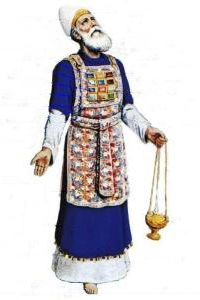
\includegraphics[width=50mm,scale=1.5]{Extras/Melchisedec.jpg}
\vspace{0.4in}  % Create a title for the document and write it in bold font
\LARGE{\textbf{\date}} % Again, do a line break
\linebreak 
% Create a subtitle \large{with Outlines, Statistics, Cross References, and Notes}
\vspace{0.5in}
\begin{flushleft}
\LARGE{Day \#81: Tuesday, 22  March 2022  \\}\vspace{0.25in}
\LARGE{Ruth 3-4 Psalm 81 Proverb 22}
\end{flushleft}
\vspace{0.6in}
\bigskip

\normalsize{Xenia, Oh.\\}
\normalsize{created: \today}
\vspace{1.3in}

\end{flushright}
\end{titlepage}

\newpage 
\tableofcontents\hypertarget{TOC}{}
\listoffigures
\listoftables

\hyphenation{A-bim-e-lech bre-thren E-phra-im  Gib-e-o-nites Jer-u-sa-lem through-out Phil-i-stines The-o-phil-us Am-a-le-kites ven-geance Mesh-el-e-mi-ah onan-ism Phar-a-oh thoughts grev-ous-ness Hach-a-liah adul-ter-er Shad-rach}

%%%%%%%%%%%%%%%%% EXTRA COLORS
%%%%%%%%%%%%%%%%% EXTRA COLORS
%%%%%%%%%%%%%%%%% EXTRA COLORS
\definecolor{champagne}{rgb}{0.97,0.91,0.81}
\definecolor{bone}{rgb}{0.89,0.85,0.79}

\definecolor{ForestGreen}{rgb}{0.00,0.29,0.098}
\definecolor{GIVING}{cmyk}{1,0.0,0.72,.1}

\definecolor{MLPE}{cmyk}{1,1,0,.45}
\definecolor{SOCCER}{cmyk}{.77, 0, .42, .49}
\definecolor{PAYBILL}{cmyk}{0,0.83,0.76,0.07}
\definecolor{SERMON}{cmyk}{.14,.9,0,.30} % aka seance \href{http://www.flatuicolorpicker.com/purple-cmyk-color-model/}{seance}
\definecolor{BIBLE}{cmyk}{0,.17,.74,.17}
\definecolor{WORKBLUE}{cmyk}{1, .5, 0, .6}
\definecolor{myOrange}{cmyk}{0, .4, .98, .03}
\definecolor{myTan}{cmyk}{0.0,.07,.17,.10}
\definecolor{myRed}{cmyk}{0,1,1,0}
\definecolor{myWhite}{cmyk}{0,0,0,0}
\definecolor{BLUESoD}{cmyk}{.97,.84,0,.04}
\definecolor{WHITE}{cmyk}{0,0,0,0}
\definecolor{OLDGOLD}{cmyk}{0.05,0.3,1.00,0}
\definecolor{CASTLETON}{cmyk}{1,0,0.31,0.66}
\definecolor{cadmiumgreen}{rgb}{0.0, 0.42, 0.24}
\definecolor{jungle}{rgb}{0.203,0.4882,0.1718}
\definecolor{MYGOLD}{rgb}{1,.84,0}

\definecolor{MYLIGHTGRAY}{rgb}{.85,.85,.85}

\definecolor{codegreen}{rgb}{0,0.6,0}
\definecolor{codegray}{rgb}{0.5,0.5,0.5}
\definecolor{codepurple}{rgb}{0.58,0,0.82}
\definecolor{backcolour}{rgb}{0.95,0.95,0.92}


\mdfdefinestyle{MyFrame}{%
    linecolor=blue,
    outerlinewidth=2pt,
    roundcorner=5pt,
    innertopmargin=\baselineskip,
    innerbottommargin=\baselineskip,
    innerrightmargin=10pt,
    innerleftmargin=10pt,
    backgroundcolor=gray!25!white}


\mdfdefinestyle{MyFrame2}{%
    linecolor=black,
    outerlinewidth=2pt,
    roundcorner=5pt,
    innertopmargin=\baselineskip,
    innerbottommargin=\baselineskip,
    innerrightmargin=10pt,
    innerleftmargin=10pt,
    backgroundcolor=yellow!25!white}


%%%%%
%% for PFTTIS list
%%%%%

%%% And Joseph said unto
\index[PFTTIS]{And Joseph said unto!Genesis!Gen 40:008}
\index[PFTTIS]{And Joseph said unto!Genesis!Gen 40:012}
\index[PFTTIS]{And Joseph said unto!Genesis!Gen 41:025}
\index[PFTTIS]{And Joseph said unto!Genesis!Gen 42:014}
\index[PFTTIS]{And Joseph said unto!Genesis!Gen 42:018}
\index[PFTTIS]{And Joseph said unto!Genesis!Gen 44:015}
\index[PFTTIS]{And Joseph said unto!Genesis!Gen 45:003}
\index[PFTTIS]{And Joseph said unto!Genesis!Gen 45:004}
\index[PFTTIS]{And Joseph said unto!Genesis!Gen 46:031}
\index[PFTTIS]{And Joseph said unto!Genesis!Gen 48:009}
\index[PFTTIS]{And Joseph said unto!Genesis!Gen 48:018}
\index[PFTTIS]{And Joseph said unto!Genesis!Gen 50:019}
\index[PFTTIS]{And Joseph said unto!Genesis!Gen 50:024}


%%% a shadow
\index[PFTTIS]{a shadow!1Chronicles!1Chr 029:15}
\index[PFTTIS]{a shadow!Job!Job 008:09}
\index[PFTTIS]{a shadow!Job!Job 014:02}
\index[PFTTIS]{a shadow!Job!Job 017:07}
\index[PFTTIS]{a shadow!Psalm!Psa 102:011}
\index[PFTTIS]{a shadow!Psalm!Psa 144:004}
\index[PFTTIS]{a shadow!Ecclesiastes!Eccl 006:012}
\index[PFTTIS]{a shadow!Ecclesiastes!Eccl 008:013}
\index[PFTTIS]{a shadow!Isaiah!Isa 04:006}
\index[PFTTIS]{a shadow!Isaiah!Isa 25:004}
\index[PFTTIS]{a shadow!Jonah!Jnh 04:06}
\index[PFTTIS]{a shadow!Colossians!Col 02:017}
\index[PFTTIS]{a shadow!Hebews!Heb 10:001}

%%% blessed is the man
\index[PFTTIS]{blessed is the man!Psalm!Psa 001:001}
\index[PFTTIS]{blessed is the man!Psalm!Psa 032:002}
\index[PFTTIS]{blessed is the man!Psalm!Psa 034:008}
\index[PFTTIS]{blessed is the man!Psalm!Psa 065:004}
\index[PFTTIS]{blessed is the man!Psalm!Psa 084:005}
\index[PFTTIS]{blessed is the man!Psalm!Psa 084:012}
\index[PFTTIS]{blessed is the man!Psalm!Psa 094:012}
\index[PFTTIS]{blessed is the man!Psalm!Psa 112:001}
\index[PFTTIS]{blessed is the man!Proverbs!Pro 008:034}
\index[PFTTIS]{blessed is the man!Isaiah!Isa 056:002}
\index[PFTTIS]{blessed is the man!Jeremiah!Jer 017:007}
\index[PFTTIS]{blessed is the man!Romans!Rom 004:008}
\index[PFTTIS]{blessed is the man!James!Jam 001:012}


%%% carry them
\index[PFTTIS]{carry them!Leviticus!Lev 14:045}
\index[PFTTIS]{carry them!Numbers!Num 11:012}
\index[PFTTIS]{carry them!Joshua!Jsh 04:003}
\index[PFTTIS]{carry them!1Samuel!1Sam 20:040}
\index[PFTTIS]{carry them!1Kings!1Kng 08:046}
\index[PFTTIS]{carry them!2Chronicles!2Chr 06:036}
\index[PFTTIS]{carry them!Ezra!Ezra 05:015}
\index[PFTTIS]{carry them!Isaiah!Isa 40:011}
\index[PFTTIS]{carry them!Isaiah!Isa 41:016}
\index[PFTTIS]{carry them!Isaiah!Isa 57:013}
\index[PFTTIS]{carry them!Jeremiah!Jer 20:004}
\index[PFTTIS]{carry them!Jeremiah!Jer 20:005}
\index[PFTTIS]{carry them!Jeremiah!Jer 43:012}


\index[PFTTIS]{good tidings!2Samuel!2Sam 18:027}
\index[PFTTIS]{good tidings!1Kings!1Ki 01:042}
\index[PFTTIS]{good tidings!2Kings!2Ki 07:009 (2x)}
\index[PFTTIS]{good tidings!Isaiah!Isa 40:009 (2x)}
\index[PFTTIS]{good tidings!Isaiah!Isa 41:007}
\index[PFTTIS]{good tidings!Isaiah!Isa 52:007}
\index[PFTTIS]{good tidings!Isaiah!Isa 61:001}
\index[PFTTIS]{good tidings!Nahum!Nah 01:005}
\index[PFTTIS]{good tidings!Luke!Lk 02:010}
\index[PFTTIS]{good tidings!1Thessalonians!1Thess 03:006}


%%% dead body
\index[PFTTIS]{dead body!Leviticus!Lev 21:011}
\index[PFTTIS]{dead body!Numbers!Num 06:006}
\index[PFTTIS]{dead body!Numbers!Num 09:006}
\index[PFTTIS]{dead body!Numbers!Num 09:007}
\index[PFTTIS]{dead body!Numbers!Num 09:010}
\index[PFTTIS]{dead body!Numbers!Num 09:011}
\index[PFTTIS]{dead body!Numbers!Num 09:013}
\index[PFTTIS]{dead body!Numbers!Num 09:016}
\index[PFTTIS]{dead body!2Kings!2Ki 08:005}
\index[PFTTIS]{dead body!Isaiah!Isa 26:019}
\index[PFTTIS]{dead body!Jeremiah!Jer 26:023}
\index[PFTTIS]{dead body!Jeremiah!Jer 36:030}
\index[PFTTIS]{dead body!Haggai!Hag 02:013}

%%% great sea
\index[PFTTIS]{great sea!Numbers!Num 34:006}
\index[PFTTIS]{great sea!Numbers!Num 34:007}
\index[PFTTIS]{great sea!Joshua!Jos 01:004}
\index[PFTTIS]{great sea!Joshua!Jos 09:001}
\index[PFTTIS]{great sea!Joshua!Jos 15:012}
\index[PFTTIS]{great sea!Joshua!Jos 15:047}
\index[PFTTIS]{great sea!Joshua!Jos 23:004}
\index[PFTTIS]{great sea!Ezekiel!Eze 47:010}
\index[PFTTIS]{great sea!Ezekiel!Eze 47:015}
\index[PFTTIS]{great sea!Ezekiel!Eze 47:019}
\index[PFTTIS]{great sea!Ezekiel!Eze 47:020}
\index[PFTTIS]{great sea!Ezekiel!Eze 48:028}
\index[PFTTIS]{great sea!Daniel!Dan 07:002}


%%% have forsaken me
\index[PFTTIS]{have forsaken me!Judges!Jdg 10:013}
\index[PFTTIS]{have forsaken me!1Samuel!1Sam 08:008}
\index[PFTTIS]{have forsaken me!1Kings!1Ki 11:033}
\index[PFTTIS]{have forsaken me!2Kings!2Ki 22:017}
\index[PFTTIS]{have forsaken me!2Chronicles!2Chr 12:005}
\index[PFTTIS]{have forsaken me!2Chronicles!2Chr 34:025}
\index[PFTTIS]{have forsaken me!Jeremiah!Jer 01:016}
\index[PFTTIS]{have forsaken me!Jeremiah!Jer 02:013}
\index[PFTTIS]{have forsaken me!Jeremiah!Jer 05:007}
\index[PFTTIS]{have forsaken me!Jeremiah!Jer 05:019}
\index[PFTTIS]{have forsaken me!Jeremiah!Jer 16:011 (2x)}
\index[PFTTIS]{have forsaken me!Jeremiah!Jer 19:004}

%%% no king
\index[PFTTIS]{no king!Judges!Jdg 17:06}
\index[PFTTIS]{no king!Judges!Jdg 18:01}
\index[PFTTIS]{no king!Judges!Jdg 19:01}
\index[PFTTIS]{no king!Judges!Jdg 21:25}
\index[PFTTIS]{no king!1Kings!1Ki 22:47}
\index[PFTTIS]{no king!2Kings!2Ki 23:25}
\index[PFTTIS]{no king!Nehemiah!Neh 13:26}
\index[PFTTIS]{no king!Psalms!Psa 033:016}
\index[PFTTIS]{no king!Proverbs!Pro 30:27}
\index[PFTTIS]{no king!Daniel!Dan 02:10}
\index[PFTTIS]{no king!Hosea!Hos 10:03}
\index[PFTTIS]{no king!Micah!Mic 04:09}
\index[PFTTIS]{no king!John!Jhn 19:15}


%%% rebellious house
\index[PFTTIS]{rebellious house!Exodus!Exo 02:005}
\index[PFTTIS]{rebellious house!Exodus!Exo 02:006}
\index[PFTTIS]{rebellious house!Exodus!Exo 02:008}
\index[PFTTIS]{rebellious house!Exodus!Exo 03:009}
\index[PFTTIS]{rebellious house!Exodus!Exo 03:026}
\index[PFTTIS]{rebellious house!Exodus!Exo 03:027}
\index[PFTTIS]{rebellious house!Exodus!Exo 12:002 (2x)}
\index[PFTTIS]{rebellious house!Exodus!Exo 12:003}
\index[PFTTIS]{rebellious house!Exodus!Exo 12:009}
\index[PFTTIS]{rebellious house!Exodus!Exo 12:025}
\index[PFTTIS]{rebellious house!Exodus!Exo 17:012}
\index[PFTTIS]{rebellious house!Exodus!Exo 24:003}

%%% seek him
\index[PFTTIS]{seek him!Deuteronomy!Deu 04:029}\index[PFTTIS]{seek him!1Samuel!1Sam 23:025}
\index[PFTTIS]{seek him!1Chronicles!1Chr 28:009}
\index[PFTTIS]{seek him!2Chronicles!1Chr 15:002}
\index[PFTTIS]{seek him!Ezra!Ezr 08:022}
\index[PFTTIS]{seek him!Psalms!Psa 022:026}
\index[PFTTIS]{seek him!Psalms!Psa 024:006}
\index[PFTTIS]{seek him!Psalms!Psa 119:002}
\index[PFTTIS]{seek him!SoS!SoS 03:002}
\index[PFTTIS]{seek him!SoS!SoS 06:001}
\index[PFTTIS]{seek him!Hosea!Hos 07:010}
\index[PFTTIS]{seek him!Amos!Amo 05:008}
\index[PFTTIS]{seek him!Hebrews!Heb 11:0063}


%%% seek ye
\index[PFTTIS]{seek ye!Isaiah!Isa 34:016}
\index[PFTTIS]{seek ye!Isaiah!Isa 45:019}
\index[PFTTIS]{seek ye!Isaiah!Isa 55:006}
\index[PFTTIS]{seek ye!Amos!Amos 5:004}
\index[PFTTIS]{seek ye!John!John 1:38}
\index[PFTTIS]{seek ye!John!John 18:4}
\index[PFTTIS]{seek ye!John!John 18:7}
\index[PFTTIS]{seek ye!Matthew!Matt 6:33}
\index[PFTTIS]{seek ye!Numbers!Num 16:10}
\index[PFTTIS]{seek ye!Luke!Luke 12:31}
\index[PFTTIS]{seek ye!Luke!Luke 24:5}
\index[PFTTIS]{seek ye!Psalm!Psa 27:8}
\index[PFTTIS]{seek ye!Zephaniah!Zeph 2:3}

%%% the uncircumcised
\index[PFTTIS]{the uncircumcised!Genesis!Gen 17:014}
\index[PFTTIS]{the uncircumcised!Judges!Jdg 14:003}
\index[PFTTIS]{the uncircumcised!Judges!Jdg 15:018}
\index[PFTTIS]{the uncircumcised!2Samuel!2Sam 01:020}
\index[PFTTIS]{the uncircumcised!Isaiah!Isa 02:001}
\index[PFTTIS]{the uncircumcised!Jeremiah!Jer 09:025}
\index[PFTTIS]{the uncircumcised!Ezekiel!Eze 28:010}
\index[PFTTIS]{the uncircumcised!Ezekiel!Eze 31:018}
\index[PFTTIS]{the uncircumcised!Ezekiel!Eze 32:019}
\index[PFTTIS]{the uncircumcised!Ezekiel!Eze 32:027}
\index[PFTTIS]{the uncircumcised!Ezekiel!Eze 32:028}
\index[PFTTIS]{the uncircumcised!Ezekiel!Eze 32:029}
\index[PFTTIS]{the uncircumcised!Ezekiel!Eze 32:032}

%%% worship him
\index[PFTTIS]{worship him!Psalms!Psa 97:007}
\index[PFTTIS]{worship him!Zephaniah!Zeph 02:011}
\index[PFTTIS]{worship him!Matthew!Matt 02:002}
\index[PFTTIS]{worship him!Matthew!Matt 02:008}
\index[PFTTIS]{worship him!John!John 04:023}
\index[PFTTIS]{worship him!John!John 04:024 (2x)} 
\index[PFTTIS]{worship him!Acts!Acts 17:023}
\index[PFTTIS]{worship him!Hebrews!Heb 01:006}
\index[PFTTIS]{worship him!Revelation!Rev 04:010}
\index[PFTTIS]{worship him!Revelation!Rev 13:008}
\index[PFTTIS]{worship him!Revelation!Rev 14:007}
\index[PFTTIS]{worship him!Revelation!Rev 19:010}


%%%%%
%% for PFTTIS list
%%%%%

%%% afflictions
\index[WFTTIS]{afflictions!Psalms!Psa 34:019}
\index[WFTTIS]{afflictions!Psalms!Psa 132:001}
\index[WFTTIS]{afflictions!Acts!Acts 07:010}
\index[WFTTIS]{afflictions!Acts!Acts 20:023}
\index[WFTTIS]{afflictions!2Corinthians!2Cor 06:004}
\index[WFTTIS]{afflictions!Colossians!Col 01:024}
\index[WFTTIS]{afflictions!1Thessalonians!1Thess 03:003}
\index[WFTTIS]{afflictions!2Timothy!2Tim 01:008}
\index[WFTTIS]{afflictions!2Timothy!2Tim 03:011}
\index[WFTTIS]{afflictions!2Timothy!2Tim 04:005}
\index[WFTTIS]{afflictions!Hebrews!Heb 10:032}
\index[WFTTIS]{afflictions!Hebrews!Heb 10:033}
\index[WFTTIS]{afflictions!1Peter!1Pet 05:009}

%%% acsend
\index[WFTTIS]{acsend!Joshua!Jos 06:05}
\index[WFTTIS]{acsend!Psalm!Psa 024:003}
\index[WFTTIS]{acsend!Psalm!Psa 135:007}
\index[WFTTIS]{acsend!Psalm!Psa 139:008}
\index[WFTTIS]{acsend!Isaiah!Isa 14:013}
\index[WFTTIS]{acsend!Isaiah!Isa 14:014}
\index[WFTTIS]{acsend!Jeremiah!Jer 10:013}
\index[WFTTIS]{acsend!Jeremiah!Jer 51:016}
\index[WFTTIS]{acsend!Ezekiel!Eze 38:009}
\index[WFTTIS]{acsend!John!John 06:062}
\index[WFTTIS]{acsend!John!John 20:017}
\index[WFTTIS]{acsend!Romans!Rom 10:006}
\index[WFTTIS]{acsend!Revelation!Rev 17:008}

%%% Assyrian
\index[WFTTIS]{Assyrian!Isaiah!Isa 10:005}
\index[WFTTIS]{Assyrian!Isaiah!Isa 10:024}
\index[WFTTIS]{Assyrian!Isaiah!Isa 14:025}
\index[WFTTIS]{Assyrian!Isaiah!Isa 19:023}
\index[WFTTIS]{Assyrian!Isaiah!Isa 23:013}
\index[WFTTIS]{Assyrian!Isaiah!Isa 30:031}
\index[WFTTIS]{Assyrian!Isaiah!Isa 31:008}
\index[WFTTIS]{Assyrian!Isaiah!Isa 52:004}
\index[WFTTIS]{Assyrian!Ezekiel!Eze 31:003}
\index[WFTTIS]{Assyrian!Hosea!Hos 05:013}
\index[WFTTIS]{Assyrian!Hosea!Hos 11:005}
\index[WFTTIS]{Assyrian!Micah!Hos 05:005}
\index[WFTTIS]{Assyrian!Micah!Hos 05:006}

%%% blot
\index[WFTTIS]{blot!Exodus!Exo 32:032}
\index[WFTTIS]{blot!Exodus!Exo 32:033}
\index[WFTTIS]{blot!Numbers!Num 05:026}
\index[WFTTIS]{blot!Deuteronomy!Deut 09:014}
\index[WFTTIS]{blot!Deuteronomy!Deut 25:019}
\index[WFTTIS]{blot!Deuteronomy!Deut 29:020}
\index[WFTTIS]{blot!2Kings!2Ki 14:027}
\index[WFTTIS]{blot!Job!Job 31:007}
\index[WFTTIS]{blot!Psalms!Psa 51:001}
\index[WFTTIS]{blot!Psalms!Psa 51:009}
\index[WFTTIS]{blot!Proverbs!Pro 09:007}
\index[WFTTIS]{blot!Jeremiah!Jer 18:023}
\index[WFTTIS]{blot!Revelation!Rev 03:005}


%%% chain
\index[WFTTIS]{chain!Genesis!Gen 41:042}
\index[WFTTIS]{chain!1Kings!1Ki 07:017}
\index[WFTTIS]{chain!Psalms!Psa 73:006}
\index[WFTTIS]{chain!SoS!Sos 04:009}
\index[WFTTIS]{chain!Lamentations!Lam 03:007}
\index[WFTTIS]{chain!Ezekiel!Eze 07:023}
\index[WFTTIS]{chain!Ezekiel!Eze 16:011}
\index[WFTTIS]{chain!Daniel!Dan 05:007}
\index[WFTTIS]{chain!Daniel!Dan 05:016}
\index[WFTTIS]{chain!Daniel!Dan 05:029}
\index[WFTTIS]{chain!Acts!Acts 28:020}
\index[WFTTIS]{chain!2Timothy!2Tim 01:016}
\index[WFTTIS]{chain!Revelation!Rev 20:001}


%%% controversy
\index[WFTTIS]{controversy!Deuteronomy!Deu 17:008}
\index[WFTTIS]{controversy!Deuteronomy!Deu 19:017}
\index[WFTTIS]{controversy!Deuteronomy!Deu 21:005}
\index[WFTTIS]{controversy!Deuteronomy!Deu 25:001}
\index[WFTTIS]{controversy!2Samuel!2Sam 15:002}
\index[WFTTIS]{controversy!Isaiah!Isa 34:008}
\index[WFTTIS]{controversy!Jeremiah!Jer 25:031}
\index[WFTTIS]{controversy!Ezekiel!Eze 44:024}
\index[WFTTIS]{controversy!Hosea!Hos 04:001}
\index[WFTTIS]{controversy!Hosea!Hos 12:002}
\index[WFTTIS]{controversy!Micah!Mic 06:002 (2x)}
\index[WFTTIS]{controversy!1Timothy!1Tim 03:016}


%%% Dagon/Dagon's
\index[WFTTIS]{Dagon!Judges!Jdg 16:023}
\index[WFTTIS]{Dagon!1Samuel!1Sam 05:002 (2x)}
\index[WFTTIS]{Dagon!1Samuel!1Sam 05:003 (2x)}
\index[WFTTIS]{Dagon!1Samuel!1Sam 05:004 (3x)}
\index[WFTTIS]{Dagon!1Samuel!1Sam 05:005 (3x)}
\index[WFTTIS]{Dagon!1Samuel!1Sam 05:007}
\index[WFTTIS]{Dagon!1Chronicles!1Chr 10:010}

%%% disobedient
\index[WFTTIS]{disobedient!1Kings!1Ki 13:026}
\index[WFTTIS]{disobedient!Nehemiah!Neh 09:026}
\index[WFTTIS]{disobedient!Luke!Luke 01:017}
\index[WFTTIS]{disobedient!Acts!Acts 26:019}
\index[WFTTIS]{disobedient!Romans!Rom 01:030}
\index[WFTTIS]{disobedient!Romans!Rom 10:021}
\index[WFTTIS]{disobedient!1Timothy!1Tim 01:009}
\index[WFTTIS]{disobedient!2Timothy!2Tim 03:002}
\index[WFTTIS]{disobedient!Titus!Titus 01:016}
\index[WFTTIS]{disobedient!Titus!Titus 03:003}
\index[WFTTIS]{disobedient!1Peter!1Pet 02:007}
\index[WFTTIS]{disobedient!1Peter!1Pet 02:008}
\index[WFTTIS]{disobedient!1Peter!1Pet 03:020}


%%% doubt
\index[WFTTIS]{doubt!Genesis!Gen 37:033}
\index[WFTTIS]{doubt!Deuteronomy!Deu 28:066}
\index[WFTTIS]{doubt!Job!Job 12:002}
\index[WFTTIS]{doubt!Matthew!Matt 14:031}
\index[WFTTIS]{doubt!Matthew!Matt 21:021}
\index[WFTTIS]{doubt!Mark!Mk 11:023}
\index[WFTTIS]{doubt!Luke!Lk 11:020}
\index[WFTTIS]{doubt!John!Jhn 10:024}
\index[WFTTIS]{doubt!Acts!Acts 02:012}
\index[WFTTIS]{doubt!Acts!Acts 28:004}
\index[WFTTIS]{doubt!1Corinthians!1Cor 09:010}
\index[WFTTIS]{doubt!Galatians!Gal 04:020}
\index[WFTTIS]{doubt!1John!1Jhn 02:019}


%%% dungeon
\index[WFTTIS]{dungeon!Genesis!Gen 40:015}
\index[WFTTIS]{dungeon!Genesis!Gen 41:014}
\index[WFTTIS]{dungeon!Exodus!Exo 12:029}
\index[WFTTIS]{dungeon!Jeremiah!Jer 37:016}
\index[WFTTIS]{dungeon!Jeremiah!Jer 38:006 (2x)}
\index[WFTTIS]{dungeon!Jeremiah!Jer 38:007}
\index[WFTTIS]{dungeon!Jeremiah!Jer 38:009}
\index[WFTTIS]{dungeon!Jeremiah!Jer 38:010}
\index[WFTTIS]{dungeon!Jeremiah!Jer 38:011}
\index[WFTTIS]{dungeon!Jeremiah!Jer 38:013}
\index[WFTTIS]{dungeon!Lamentations!Lam 03:053}
\index[WFTTIS]{dungeon!Lamentations!Lam 03:055}


%%% error
\index[WFTTIS]{error!2Samuel!2Sam 06:007}
\index[WFTTIS]{error!Job!Job 19:004}
\index[WFTTIS]{error!Ecclesiastes!Ecc 05:006}
\index[WFTTIS]{error!Ecclesiastes!Ecc 10:005}
\index[WFTTIS]{error!Isaiah!Isa 32:006}
\index[WFTTIS]{error!Daniel!Dan 06:004}
\index[WFTTIS]{error!Matthew!Matt 27:064}
\index[WFTTIS]{error!Romans!Rom 01:027}
\index[WFTTIS]{error!James!Jam 05:020}
\index[WFTTIS]{error!2Peter!2Pet 02:018}
\index[WFTTIS]{error!2Peter!2Pet 03:017}
\index[WFTTIS]{error!1John!1Jn 04:006}
\index[WFTTIS]{error!Jude!Jude 01:011}

%%% fourish
\index[WFTTIS]{fourish!Psalms!Psa 072:007}
\index[WFTTIS]{fourish!Psalms!Psa 072:016}
\index[WFTTIS]{fourish!Psalms!Psa 092:007}
\index[WFTTIS]{fourish!Psalms!Psa 092:012}
\index[WFTTIS]{fourish!Psalms!Psa 092:013}
\index[WFTTIS]{fourish!Psalms!Psa 132:018}
\index[WFTTIS]{fourish!Proverbs!Pro 11:28}
\index[WFTTIS]{fourish!Proverbs!Pro 14:11}
\index[WFTTIS]{fourish!Ecclesiastes!Ecc 12:05}
\index[WFTTIS]{fourish!SongOfSolomon!SOS 07:12}
\index[WFTTIS]{fourish!Isaiah!Isa 17:11}
\index[WFTTIS]{fourish!Isaiah!Isa 66:14}
\index[WFTTIS]{fourish!Ezekiel!Eze 17:24}




%%% giants
\index[WFTTIS]{giants!Genesis!Gen 06:004}
\index[WFTTIS]{giants!Numbers!Num 13:033}
\index[WFTTIS]{giants!Deuteronomy!Deut 02:011}
\index[WFTTIS]{giants!Deuteronomy!Deut 02:021}
\index[WFTTIS]{giants!Deuteronomy!Deut 03:011}
\index[WFTTIS]{giants!Deuteronomy!Deut 03:013}
\index[WFTTIS]{giants!Joshua!Josh 12:004}
\index[WFTTIS]{giants!Joshua!Josh 13:012}
\index[WFTTIS]{giants!Joshua!Josh 15:008}
\index[WFTTIS]{giants!Joshua!Josh 17:015}
\index[WFTTIS]{giants!Joshua!Josh 16:016}

%%% good man
\index[WFTTIS]{good man!2 Samuel!2Sa 18:27}
%(1) Psalms 37:23 [5]
%(1) Psalms 112:5 [2]
%(1) Proverbs 12:2 [2]
%(1) Proverbs 13:22 [2]
%(1) Proverbs 14:14 [14]
%(1) Micah 7:2 [2]
%(1) Matthew 12:35 [2]
%(1) Luke 6:45 [2]
%(1) Luke 23:50 [15]
%(1) John 7:12 [17]
%(1) Acts 11:24 [5]
%(1) Romans 5:7 [14]

%%% Hinnom
\index[WFTTIS]{Hinnom!Joshua!Jsh 15:008}
\index[WFTTIS]{Hinnom!Joshua!Jsh 18:016}
\index[WFTTIS]{Hinnom!2Kings!2Ki 23:010}
\index[WFTTIS]{Hinnom!2Chronicles!2Chr 28:003}
\index[WFTTIS]{Hinnom!2Chronicles!2Chr 33:006}
\index[WFTTIS]{Hinnom!Nehemiah!Neh 11:030}
\index[WFTTIS]{Hinnom!Jeremiah!Jer 07:031}
\index[WFTTIS]{Hinnom!Jeremiah!Jer 07:032}
\index[WFTTIS]{Hinnom!Jeremiah!Jer 19:002}
\index[WFTTIS]{Hinnom!Jeremiah!Jer 19:006}
\index[WFTTIS]{Hinnom!Jeremiah!Jer 32:035}

%%% inclined
\index[WFTTIS]{inclined!Judges!Jdg 09:003}
\index[WFTTIS]{inclined!Psalms!Psa 040:001}
\index[WFTTIS]{inclined!Psalms!Psa 116:002}
\index[WFTTIS]{inclined!Psalms!Psa 119:112}
\index[WFTTIS]{inclined!Proverbs!Pro 05:13}
\index[WFTTIS]{inclined!Jeremiah!Jer 07:24}
\index[WFTTIS]{inclined!Jeremiah!Jer 07:26}
\index[WFTTIS]{inclined!Jeremiah!Jer 11:08}
\index[WFTTIS]{inclined!Jeremiah!Jer 17:23}
\index[WFTTIS]{inclined!Jeremiah!Jer 25:04}
\index[WFTTIS]{inclined!Jeremiah!Jer 34:14}
\index[WFTTIS]{inclined!Jeremiah!Jer 35:15}
\index[WFTTIS]{inclined!Jeremiah!Jer 44:05}


%%% laughed
\index[WFTTIS]{laughed!Genesis!Gen 17:017}
\index[WFTTIS]{laughed!Genesis!Gen 18:012}
\index[WFTTIS]{laughed!Genesis!Gen 18:015}
\index[WFTTIS]{laughed!2Kings!2Ki 19:021}
\index[WFTTIS]{laughed!2Chronicles!2Chr 30:010}
\index[WFTTIS]{laughed!Nehemiah!Neh 02:019}
\index[WFTTIS]{laughed!Job!Job 12:004}
\index[WFTTIS]{laughed!Job!Job 29:024}
\index[WFTTIS]{laughed!Isaiah!Isa 37:022}
\index[WFTTIS]{laughed!Ezekiel!Ezek 23:032}
\index[WFTTIS]{laughed!Matthew!Matt 09:024}
\index[WFTTIS]{laughed!Mark!Mk 05:040}
\index[WFTTIS]{laughed!Luke!Lk 08:053}

%%% liar
\index[WFTTIS]{liar!Job!Job 24:025}
\index[WFTTIS]{liar!Proverbs!Pro 17:004}
\index[WFTTIS]{liar!Proverbs!Pro 19:022}
\index[WFTTIS]{liar!Proverbs!Pro 30:006}
\index[WFTTIS]{liar!Jeremiah!Jer 15:018}
\index[WFTTIS]{liar!John!Jhn 08:044}
\index[WFTTIS]{liar!John!Jhn 08:055}
\index[WFTTIS]{liar!Romans!Rom 03:004}
\index[WFTTIS]{liar!1John!1Jhn 01:010}
\index[WFTTIS]{liar!1John!1Jhn 02:004}
\index[WFTTIS]{liar!1John!1Jhn 02:022}
\index[WFTTIS]{liar!1John!1Jhn 04:020}
\index[WFTTIS]{liar!1John!1Jhn 05:010}

%%% palsy
\index[WFTTIS]{palsy!Matthew!Matt 04:024}
\index[WFTTIS]{palsy!Matthew!Matt 08:006}
\index[WFTTIS]{palsy!Matthew!Matt 09:002}
\index[WFTTIS]{palsy!Matthew!Matt 09:006}
\index[WFTTIS]{palsy!Mark!Mk 02:003}
\index[WFTTIS]{palsy!Mark!Mk 02:004}
\index[WFTTIS]{palsy!Mark!Mk 02:005}
\index[WFTTIS]{palsy!Mark!Mk 02:009}
\index[WFTTIS]{palsy!Mark!Mk 02:010}
\index[WFTTIS]{palsy!Luke!Lk 05:018}
\index[WFTTIS]{palsy!Luke!Lk 05:024}
\index[WFTTIS]{palsy!Acts!Acts 09:033}

%%% Profitable
\index[WFTTIS]{profitable!Job!Job 22:002 (2x)}
\index[WFTTIS]{profitable!Ecclesiastes!Ecc 10:010}
\index[WFTTIS]{profitable!Isaiah!Isa 44:010}
\index[WFTTIS]{profitable!Jeremiah!Jer 13:007}
\index[WFTTIS]{profitable!Matthew!Matt 05:029}
\index[WFTTIS]{profitable!Matthew!Matt 05:030}
\index[WFTTIS]{profitable!Acts!Acts 20:020}
\index[WFTTIS]{profitable!1Timothy!1Tim 04:008}
\index[WFTTIS]{profitable!2Timothy!2Tim 03:016}
\index[WFTTIS]{profitable!2Timothy!2Tim 04:011}
\index[WFTTIS]{profitable!Titus!Titus 03:008}
\index[WFTTIS]{profitable!Philemon!Phlm 01:011}

%%% Rechab
\index[WFTTIS]{Rechab!2Samuel!2Sam 04:002}
\index[WFTTIS]{Rechab!2Samuel!2Sam 04:005}
\index[WFTTIS]{Rechab!2Samuel!2Sam 04:006}
\index[WFTTIS]{Rechab!2Samuel!2Sam 04:009}
\index[WFTTIS]{Rechab!2KIngs!2Ki 10:015}
\index[WFTTIS]{Rechab!2KIngs!2Ki 10:023}
\index[WFTTIS]{Rechab!1Chronicles!1Chr 02:055}
\index[WFTTIS]{Rechab!Nehemiah!Neh 03:014}
\index[WFTTIS]{Rechab!Jeremiah!Jer 35:006}
\index[WFTTIS]{Rechab!Jeremiah!Jer 35:008}
\index[WFTTIS]{Rechab!Jeremiah!Jer 35:014}
\index[WFTTIS]{Rechab!Jeremiah!Jer 35:016}
\index[WFTTIS]{Rechab!Jeremiah!Jer 35:019}

%%% serpents
\index[WFTTIS]{serpents!Exodus!Exo 07:012}
\index[WFTTIS]{serpents!Numbers!Num 21:006}
\index[WFTTIS]{serpents!Numbers!Num 21:007}
\index[WFTTIS]{serpents!Deuteronomy!Deu 08:015}
\index[WFTTIS]{serpents!Deuteronomy!Deu 32:024}
\index[WFTTIS]{serpents!Jeremiah!Jer 08:017}
\index[WFTTIS]{serpents!Matthew!Matt 10:016}
\index[WFTTIS]{serpents!Matthew!Matt 23:033}
\index[WFTTIS]{serpents!Mark!Mk 16:018}
\index[WFTTIS]{serpents!Luke!Lk 10:019}
\index[WFTTIS]{serpents!1Corinthians!1Cor 10:009}
\index[WFTTIS]{serpents!James!Jas 03:007}
\index[WFTTIS]{serpents!Revelation!Rev 09:019}

%%% short
\index[WFTTIS]{short!Numbers!Num 11:023}
\index[WFTTIS]{short!2Kings!2Ki 10:032}
\index[WFTTIS]{short!Job!Job 17:012}
\index[WFTTIS]{short!Job!Job 20:005}
\index[WFTTIS]{short!Psalms!Psa 89:047}
\index[WFTTIS]{short!Romans!Rom 03:023}
\index[WFTTIS]{short!Romans!Rom 09:028  (2x)}
\index[WFTTIS]{short!1Corinthians!1Cor 07:029}
\index[WFTTIS]{short!1Thessalonians!1Thess 02:017}
\index[WFTTIS]{short!Hebrews!Heb 04:001}
\index[WFTTIS]{short!Revelation!Rev 12:012}
\index[WFTTIS]{short!Revelation!Rev 17:010}

%%% smiteth
\index[WFTTIS]{smiteth!Exodus!Exo 21:012}
\index[WFTTIS]{smiteth!Exodus!Exo 21:15}
\index[WFTTIS]{smiteth!Deuteronomy!Dt 25:11}
\index[WFTTIS]{smiteth!Deuteronomy!Dt 27:24}
\index[WFTTIS]{smiteth!Joshua!Jsh 15:16}
\index[WFTTIS]{smiteth!Judges!Jdg 15:16}
\index[WFTTIS]{smiteth!2 Samuel!2Sa 05:08}
\index[WFTTIS]{smiteth!1Chronicles!1Chr 11:06}
\index[WFTTIS]{smiteth!Job!1Chr 26:12}
\index[WFTTIS]{smiteth!Isaiah!Isa 09:13}
\index[WFTTIS]{smiteth!Lamentations!Lam 03:30}
\index[WFTTIS]{smiteth!Ezekiel!Eze 07:09}
\index[WFTTIS]{smiteth!Luke!Lk 06:29}



%%% vanities
\index[WFTTIS]{vanities!Deuteronomy!Deut 21:021}
\index[WFTTIS]{vanities!1Kings!1Ki 16:013}
\index[WFTTIS]{vanities!1Kings!1Ki 16:026}
\index[WFTTIS]{vanities!Psalms!Psa 031:006}
\index[WFTTIS]{vanities!Ecclesiastes!Ecc 01:002 (2x)}
\index[WFTTIS]{vanities!Ecclesiastes!Ecc 05:007}
\index[WFTTIS]{vanities!Ecclesiastes!Ecc 12:008}
\index[WFTTIS]{vanities!Jeremiah!Jer 08:019}
\index[WFTTIS]{vanities!Jeremiah!Jer 10:008}
\index[WFTTIS]{vanities!Jeremiah!Jer 14:022}
\index[WFTTIS]{vanities!Jonah!Jnh 02:008}
\index[WFTTIS]{vanities!Acts!Acts 14:015}



%%%%%
%% for PFTTIS list
%%%%%

%%% worm
\index[WFITV]{worm!Exodus!Exo 16:024}
\index[WFITV]{worm!Job!Job 17:014}
\index[WFITV]{worm!Job!Job 24:029}
\index[WFITV]{worm!Job!Job 25:005 (2x)}
\index[WFITV]{worm!Psalms!Psa 022:006}
\index[WFITV]{worm!Isaiah!Isa 14:011}
\index[WFITV]{worm!Isaiah!Isa 41:014}
\index[WFITV]{worm!Isaiah!Isa 51:008}
\index[WFITV]{worm!Isaiah!Isa 66:024}
\index[WFITV]{worm!Jonah!Jnh 04:007}
\index[WFITV]{worm!Mark!Mk 09:044}
\index[WFITV]{worm!Mark!Mk 09:046}
\index[WFITV]{worm!Mark!Mk 09:048}


%\subsubsection{Title}
%\textbf{Introduction:} Isaiah 46 
%\index[speaker]{Speaker!Isaiah 49 (Title}
%\index[series]{Book (Speaker)!IPassage (Title)}
%\index[date]{2017/07/09!Isaiah 49 (Title)}
%\begin{compactenum}[I.]
%    \item  \textbf{Point} \index[scripture]{Isaiah!IPassage} (IPassage)
%\end{compactenum}




  


%\input{02OT-Exodus/ExodusIntroduction}

%\newpage
%\begin{figure}
%\begin{center}
%\includegraphics[scale=.7, angle=0]{05OT-Deuteronomy/References/AndrewSmithDeuteronomyTimeline.png}
%\caption[Deuteronomy Timeline by Andrew Smith]{Deuteronomy Timeline by Andrew %Smith}
%\label{fig:Deuteronomy Timeline by Andrew Smith}
%\end{center}
%\end{figure}

\newpage
\begin{figure}
\begin{center}
\includegraphics[scale=0.4, angle=90]{08OT-Ruth/References/BibleProject-Ruth}
\caption[Ruth from The Bible Project]{Ruth from The Bible Project}
\label{fig:Ruth from The Bible Project}
\end{center}
\end{figure}


\newpage
\begin{figure}
\begin{center}
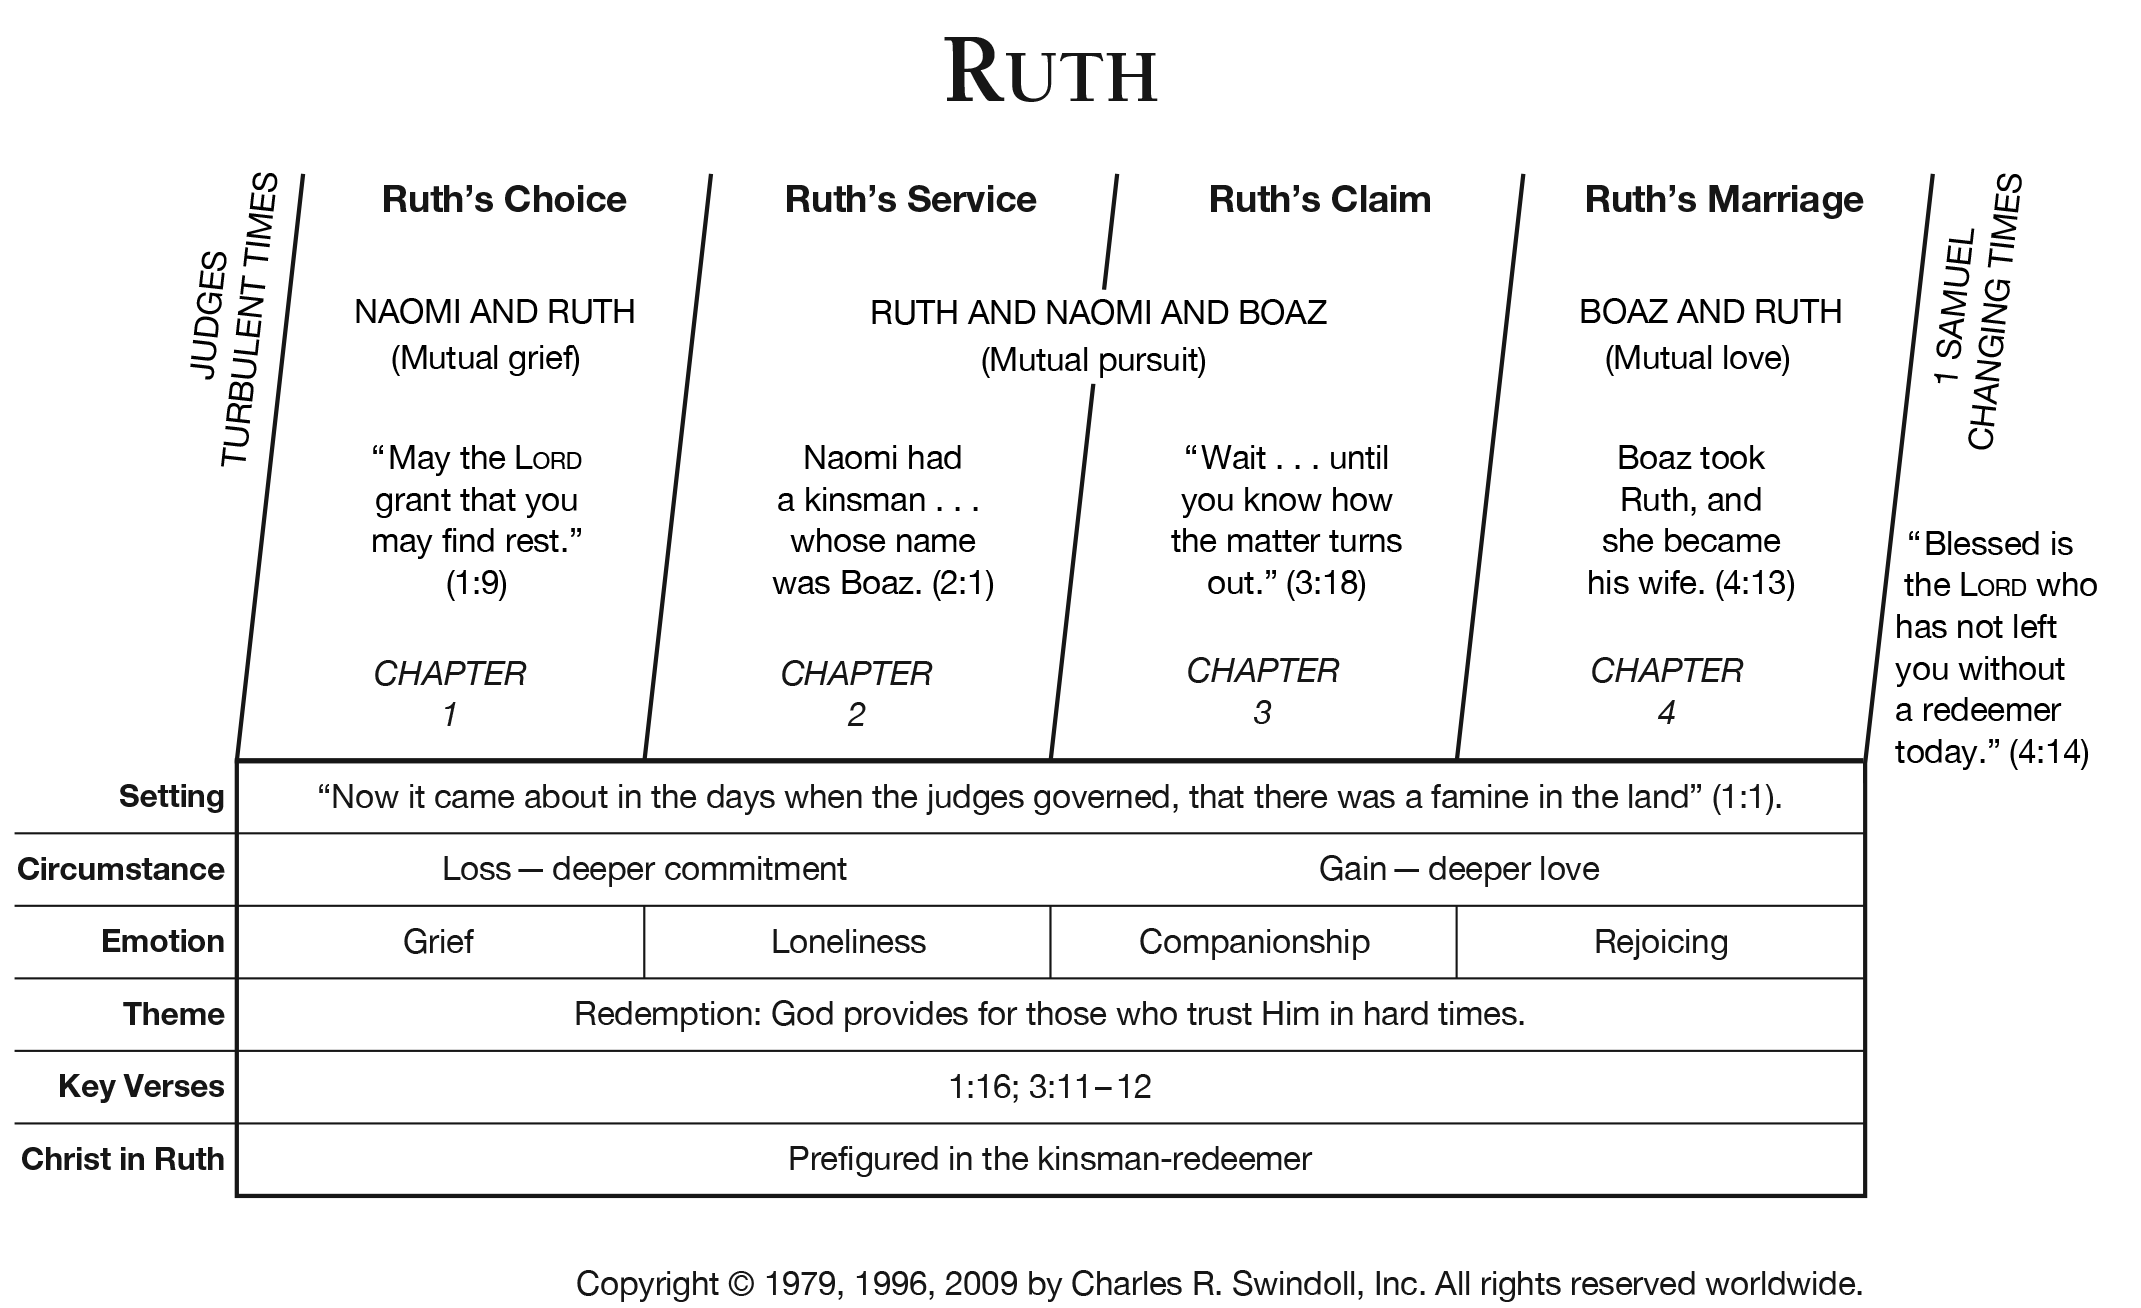
\includegraphics[scale=0.25, angle=90]{08OT-Ruth/References/Swindoll-Ruth}
\caption[Ruth from Swindoll]{Ruth from The Swindoll}
\label{fig:Ruth from Swindoll}
\end{center}
\end{figure}

\newpage
\begin{figure}
\begin{center}
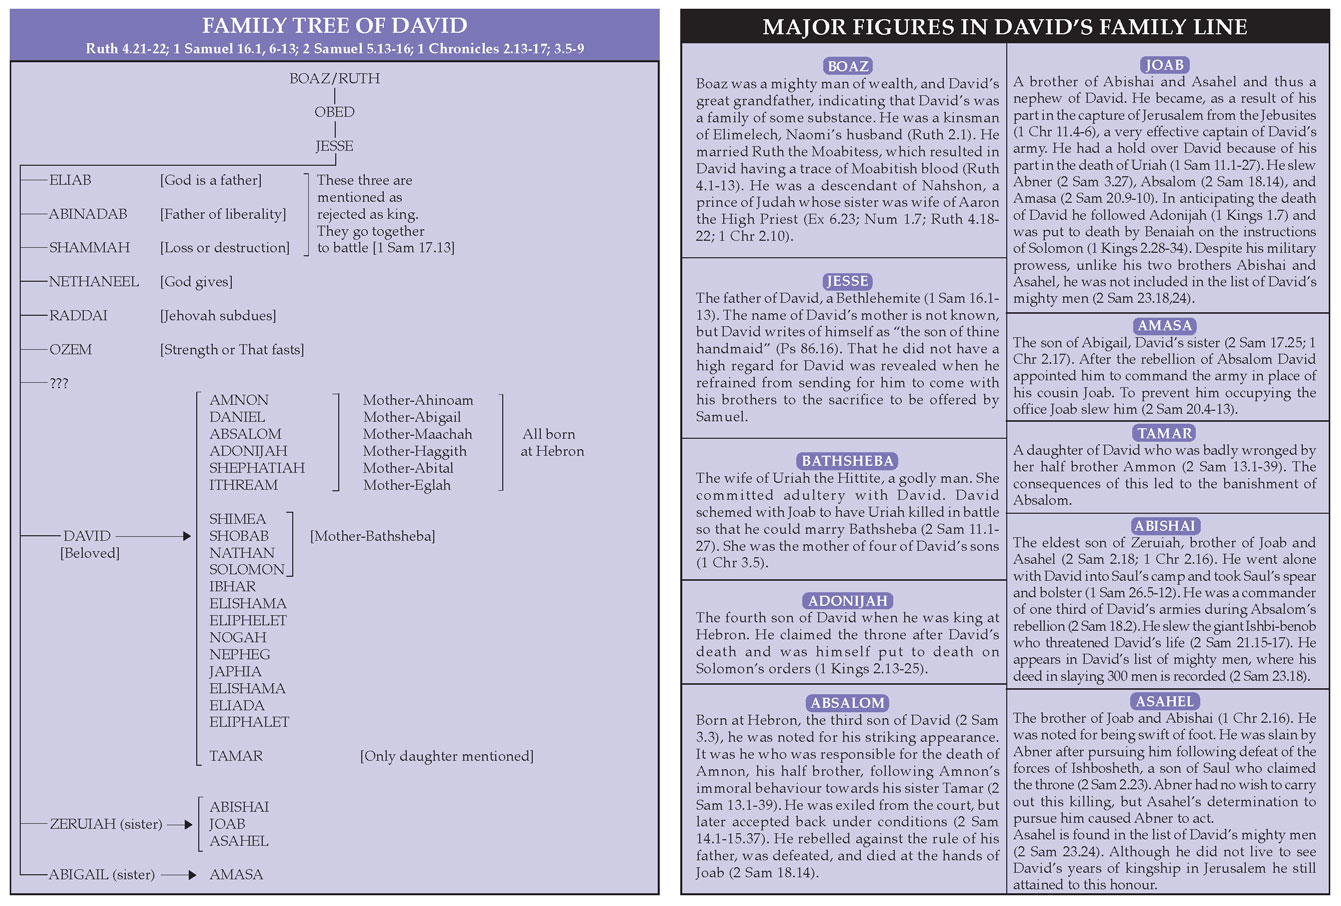
\includegraphics[scale=0.4, angle=90]{08OT-Ruth/References/JohnGrantFamilyTreeOfDavid}
\caption[The Family Tree of David]{The Family Tree of David}
\label{fig:The Family Tree of David}
\end{center}
\end{figure}


\chapter{Ruth 3}





\marginpar{\scriptsize \centering \fcolorbox{bone}{lime}{\textbf{FINDING A HUSBAND}}\\ (Ruth 3:1-18) \begin{compactenum}[I.][8]
    \item  \textbf{Rest}  \index[scripture]{Ruth!Ruth 03:01}(Ruth 3:1)
    \item The \textbf{Request} with Grace \index[scripture]{Ruth!Ruth 03:06--09}(Ruth 3:6--9)
    \item The \textbf{Reassurance} with Grace \index[scripture]{Ruth!Ruth 03:10--18--09}(Ruth 3:10--18)
    \item  The \textbf{Redeemer}  \index[scripture]{Ruth!Ruth 03:11}(Ruth 3:11)
    \item  The \textbf{Reputation}  \index[scripture]{Ruth!Ruth 03:11}(Ruth 3:11)
    \item  The \textbf{Relative}  \index[scripture]{Ruth!Ruth 03:12}(Ruth 3:12)
    \item  The \textbf{Rush}  \index[scripture]{Ruth!Ruth 03:17}(Ruth 3:17)
\end{compactenum}}







\footnote{\textcolor[cmyk]{0.99998,1,0,0}{\hyperlink{TOC}{Return to end of Table of Contents.}}}\footnote{\href{https://audiobible.com/bible/ruth_3.html}{\textcolor[cmyk]{0.99998,1,0,0}{Ruth 3 Audio}}}\textcolor[cmyk]{0.99998,1,0,0}{Then Naomi her mother in law said unto her, My daughter, shall I not seek \fcolorbox{bone}{lime}{rest} for thee, that it may be well with thee?}
[2] \textcolor[cmyk]{0.99998,1,0,0}{And now \emph{is} not Boaz of our kindred, with whose maidens thou wast? Behold, he winnoweth barley to night in the threshingfloor.}
[3] \textcolor[cmyk]{0.99998,1,0,0}{Wash thyself therefore, and anoint thee, and put thy raiment upon thee, and get thee down to the floor: \emph{but} make not thyself known unto the man, until he shall have done eating and drinking.}
[4] \textcolor[cmyk]{0.99998,1,0,0}{And it shall be, when he lieth down, that thou shalt mark the place where he shall lie, and thou shalt go in, and uncover his feet, and lay thee down; and he will tell thee what thou shalt do.}
[5] \textcolor[cmyk]{0.99998,1,0,0}{And \fcolorbox{bone}{bone}{she} said unto her, All that thou sayest unto me I will do.}\\
\\
\P \textcolor[cmyk]{0.99998,1,0,0}{And \fcolorbox{bone}{bone}{she} went down unto the floor, and did according to all that her mother in law bade her.}
[7] \textcolor[cmyk]{0.99998,1,0,0}{And when Boaz had eaten and drunk, and his heart was merry, he went to lie down at the end of the heap of corn: and \fcolorbox{bone}{bone}{she} came softly, and \fcolorbox{bone}{lime}{uncovered his feet}, and laid her down.}\\
\\
\P \textcolor[cmyk]{0.99998,1,0,0}{And it came to pass at midnight, that the man was afraid, and turned himself: and, behold, a woman lay at his feet.}
[9] \textcolor[cmyk]{0.99998,1,0,0}{And he said, Who \emph{art} thou? And \fcolorbox{bone}{bone}{she} answered, I \emph{am} Ruth thine handmaid: spread therefore thy skirt over thine handmaid; for thou \emph{art} a near kinsman.}
[10] \textcolor[cmyk]{0.99998,1,0,0}{And he said, \fcolorbox{bone}{lime}{Blessed \emph{be} thou} of the LORD, my daughter: \emph{for} thou hast shewed more kindness in the latter end than at the beginning, inasmuch as thou followedst not young men, whether poor or rich.}
[11] \textcolor[cmyk]{0.99998,1,0,0}{And now, my daughter, fear not; I will do to thee all that thou \fcolorbox{bone}{lime}{requirest}: for all the city of my people doth know that thou \emph{art} a \fcolorbox{bone}{lime}{virtuous} woman.}
[12] \textcolor[cmyk]{0.99998,1,0,0}{And now it is true that I \emph{am} \emph{thy} near kinsman: howbeit there is a kinsman nearer than I.}
[13] \textcolor[cmyk]{0.99998,1,0,0}{Tarry this night, and it shall be in the morning, \emph{that} if he will perform unto thee the part of a \fcolorbox{bone}{lime}{kinsman}, well; let him do the kinsman's part: but if he will not do the part of a kinsman to thee, then will I do the part of a kinsman to thee, \emph{as} the LORD liveth: lie down until the morning.}\\
\\
\P \textcolor[cmyk]{0.99998,1,0,0}{And \fcolorbox{bone}{bone}{she} lay at his feet until the morning: and \fcolorbox{bone}{bone}{she} rose up before one could know another. And he said, Let it not be known that a woman came into the floor.}
[15] \textcolor[cmyk]{0.99998,1,0,0}{Also he said, Bring the vail that \emph{thou} \emph{hast} upon thee, and hold it. And when \fcolorbox{bone}{bone}{she} held it, he measured six \emph{measures} of barley, and laid \emph{it} on her: and \fcolorbox{bone}{bone}{she} went into the city.}
[16] \textcolor[cmyk]{0.99998,1,0,0}{And when \fcolorbox{bone}{bone}{she} came to her mother in law, \fcolorbox{bone}{bone}{she} said, Who \emph{art} thou, my daughter? And \fcolorbox{bone}{bone}{she} told her all that the man had done to her.}
[17] \textcolor[cmyk]{0.99998,1,0,0}{And \fcolorbox{bone}{bone}{she} said, These six \emph{measures} of barley gave he me; for he said to me, \fcolorbox{bone}{lime}{Go not empty} unto thy mother in law.}
[18] \textcolor[cmyk]{0.99998,1,0,0}{Then said \fcolorbox{bone}{bone}{she}, Sit still, my daughter, until thou know how the matter will fall: for the man will not be in rest, until he have finished the thing this day.}
\index[NWIV]{25!Ruth!Rut 3:1}\index[AWIP]{Then!Ruth!Rut 3:1}\index[AWIP]{Naomi!Ruth!Rut 3:1}\index[AWIP]{her!Ruth!Rut 3:1}\index[AWIP]{her!Ruth!Rut 3:1 (2)}\index[AWIP]{mother!Ruth!Rut 3:1}\index[AWIP]{in!Ruth!Rut 3:1}\index[AWIP]{law!Ruth!Rut 3:1}\index[AWIP]{said!Ruth!Rut 3:1}\index[AWIP]{unto!Ruth!Rut 3:1}\index[AWIP]{My!Ruth!Rut 3:1}\index[AWIP]{daughter!Ruth!Rut 3:1}\index[AWIP]{shall!Ruth!Rut 3:1}\index[AWIP]{I!Ruth!Rut 3:1}\index[AWIP]{not!Ruth!Rut 3:1}\index[AWIP]{seek!Ruth!Rut 3:1}\index[AWIP]{rest!Ruth!Rut 3:1}\index[AWIP]{for!Ruth!Rut 3:1}\index[AWIP]{thee!Ruth!Rut 3:1}\index[AWIP]{that!Ruth!Rut 3:1}\index[AWIP]{it!Ruth!Rut 3:1}\index[AWIP]{may!Ruth!Rut 3:1}\index[AWIP]{be!Ruth!Rut 3:1}\index[AWIP]{well!Ruth!Rut 3:1}\index[AWIP]{with!Ruth!Rut 3:1}\index[AWIP]{thee?!Ruth!Rut 3:1}

\index[NWIV]{22!Ruth!Rut 3:2}\index[AWIP]{And!Ruth!Rut 3:2}\index[AWIP]{now!Ruth!Rut 3:2}\index[AWIP]{\emph{is}!Ruth!Rut 3:2}\index[AWIP]{not!Ruth!Rut 3:2}\index[AWIP]{Boaz!Ruth!Rut 3:2}\index[AWIP]{of!Ruth!Rut 3:2}\index[AWIP]{our!Ruth!Rut 3:2}\index[AWIP]{kindred!Ruth!Rut 3:2}\index[AWIP]{with!Ruth!Rut 3:2}\index[AWIP]{whose!Ruth!Rut 3:2}\index[AWIP]{maidens!Ruth!Rut 3:2}\index[AWIP]{thou!Ruth!Rut 3:2}\index[AWIP]{wast?!Ruth!Rut 3:2}\index[AWIP]{Behold!Ruth!Rut 3:2}\index[AWIP]{he!Ruth!Rut 3:2}\index[AWIP]{winnoweth!Ruth!Rut 3:2}\index[AWIP]{barley!Ruth!Rut 3:2}\index[AWIP]{to!Ruth!Rut 3:2}\index[AWIP]{night!Ruth!Rut 3:2}\index[AWIP]{in!Ruth!Rut 3:2}\index[AWIP]{the!Ruth!Rut 3:2}\index[AWIP]{threshingfloor!Ruth!Rut 3:2}\index[AWIP]{\emph{is}!Ruth!Rut 3:2}

\index[NWIV]{35!Ruth!Rut 3:3}\index[AWIP]{Wash!Ruth!Rut 3:3}\index[AWIP]{thyself!Ruth!Rut 3:3}\index[AWIP]{thyself!Ruth!Rut 3:3 (2)}\index[AWIP]{therefore!Ruth!Rut 3:3}\index[AWIP]{and!Ruth!Rut 3:3}\index[AWIP]{and!Ruth!Rut 3:3 (2)}\index[AWIP]{and!Ruth!Rut 3:3 (3)}\index[AWIP]{and!Ruth!Rut 3:3 (4)}\index[AWIP]{anoint!Ruth!Rut 3:3}\index[AWIP]{thee!Ruth!Rut 3:3}\index[AWIP]{thee!Ruth!Rut 3:3 (2)}\index[AWIP]{thee!Ruth!Rut 3:3 (3)}\index[AWIP]{put!Ruth!Rut 3:3}\index[AWIP]{thy!Ruth!Rut 3:3}\index[AWIP]{raiment!Ruth!Rut 3:3}\index[AWIP]{upon!Ruth!Rut 3:3}\index[AWIP]{get!Ruth!Rut 3:3}\index[AWIP]{down!Ruth!Rut 3:3}\index[AWIP]{to!Ruth!Rut 3:3}\index[AWIP]{the!Ruth!Rut 3:3}\index[AWIP]{the!Ruth!Rut 3:3 (2)}\index[AWIP]{floor!Ruth!Rut 3:3}\index[AWIP]{\emph{but}!Ruth!Rut 3:3}\index[AWIP]{make!Ruth!Rut 3:3}\index[AWIP]{not!Ruth!Rut 3:3}\index[AWIP]{known!Ruth!Rut 3:3}\index[AWIP]{unto!Ruth!Rut 3:3}\index[AWIP]{man!Ruth!Rut 3:3}\index[AWIP]{until!Ruth!Rut 3:3}\index[AWIP]{he!Ruth!Rut 3:3}\index[AWIP]{shall!Ruth!Rut 3:3}\index[AWIP]{have!Ruth!Rut 3:3}\index[AWIP]{done!Ruth!Rut 3:3}\index[AWIP]{eating!Ruth!Rut 3:3}\index[AWIP]{drinking!Ruth!Rut 3:3}\index[AWIP]{\emph{but}!Ruth!Rut 3:3}

\index[NWIV]{40!Ruth!Rut 3:4}\index[AWIP]{And!Ruth!Rut 3:4}\index[AWIP]{it!Ruth!Rut 3:4}\index[AWIP]{shall!Ruth!Rut 3:4}\index[AWIP]{shall!Ruth!Rut 3:4 (2)}\index[AWIP]{be!Ruth!Rut 3:4}\index[AWIP]{when!Ruth!Rut 3:4}\index[AWIP]{he!Ruth!Rut 3:4}\index[AWIP]{he!Ruth!Rut 3:4 (2)}\index[AWIP]{he!Ruth!Rut 3:4 (3)}\index[AWIP]{lieth!Ruth!Rut 3:4}\index[AWIP]{down!Ruth!Rut 3:4}\index[AWIP]{down!Ruth!Rut 3:4 (2)}\index[AWIP]{that!Ruth!Rut 3:4}\index[AWIP]{thou!Ruth!Rut 3:4}\index[AWIP]{thou!Ruth!Rut 3:4 (2)}\index[AWIP]{thou!Ruth!Rut 3:4 (3)}\index[AWIP]{shalt!Ruth!Rut 3:4}\index[AWIP]{shalt!Ruth!Rut 3:4 (2)}\index[AWIP]{shalt!Ruth!Rut 3:4 (3)}\index[AWIP]{mark!Ruth!Rut 3:4}\index[AWIP]{the!Ruth!Rut 3:4}\index[AWIP]{place!Ruth!Rut 3:4}\index[AWIP]{where!Ruth!Rut 3:4}\index[AWIP]{lie!Ruth!Rut 3:4}\index[AWIP]{and!Ruth!Rut 3:4}\index[AWIP]{and!Ruth!Rut 3:4 (2)}\index[AWIP]{and!Ruth!Rut 3:4 (3)}\index[AWIP]{and!Ruth!Rut 3:4 (4)}\index[AWIP]{go!Ruth!Rut 3:4}\index[AWIP]{in!Ruth!Rut 3:4}\index[AWIP]{uncover!Ruth!Rut 3:4}\index[AWIP]{his!Ruth!Rut 3:4}\index[AWIP]{feet!Ruth!Rut 3:4}\index[AWIP]{lay!Ruth!Rut 3:4}\index[AWIP]{thee!Ruth!Rut 3:4}\index[AWIP]{thee!Ruth!Rut 3:4 (2)}\index[AWIP]{will!Ruth!Rut 3:4}\index[AWIP]{tell!Ruth!Rut 3:4}\index[AWIP]{what!Ruth!Rut 3:4}\index[AWIP]{do!Ruth!Rut 3:4}

\index[NWIV]{14!Ruth!Rut 3:5}\index[AWIP]{And!Ruth!Rut 3:5}\index[AWIP]{she!Ruth!Rut 3:5}\index[AWIP]{said!Ruth!Rut 3:5}\index[AWIP]{unto!Ruth!Rut 3:5}\index[AWIP]{unto!Ruth!Rut 3:5 (2)}\index[AWIP]{her!Ruth!Rut 3:5}\index[AWIP]{All!Ruth!Rut 3:5}\index[AWIP]{that!Ruth!Rut 3:5}\index[AWIP]{thou!Ruth!Rut 3:5}\index[AWIP]{sayest!Ruth!Rut 3:5}\index[AWIP]{me!Ruth!Rut 3:5}\index[AWIP]{I!Ruth!Rut 3:5}\index[AWIP]{will!Ruth!Rut 3:5}\index[AWIP]{do!Ruth!Rut 3:5}

\index[NWIV]{19!Ruth!Rut 3:6}\index[AWIP]{And!Ruth!Rut 3:6}\index[AWIP]{she!Ruth!Rut 3:6}\index[AWIP]{went!Ruth!Rut 3:6}\index[AWIP]{down!Ruth!Rut 3:6}\index[AWIP]{unto!Ruth!Rut 3:6}\index[AWIP]{the!Ruth!Rut 3:6}\index[AWIP]{floor!Ruth!Rut 3:6}\index[AWIP]{and!Ruth!Rut 3:6}\index[AWIP]{did!Ruth!Rut 3:6}\index[AWIP]{according!Ruth!Rut 3:6}\index[AWIP]{to!Ruth!Rut 3:6}\index[AWIP]{all!Ruth!Rut 3:6}\index[AWIP]{that!Ruth!Rut 3:6}\index[AWIP]{her!Ruth!Rut 3:6}\index[AWIP]{her!Ruth!Rut 3:6 (2)}\index[AWIP]{mother!Ruth!Rut 3:6}\index[AWIP]{in!Ruth!Rut 3:6}\index[AWIP]{law!Ruth!Rut 3:6}\index[AWIP]{bade!Ruth!Rut 3:6}

\index[NWIV]{37!Ruth!Rut 3:7}\index[AWIP]{And!Ruth!Rut 3:7}\index[AWIP]{when!Ruth!Rut 3:7}\index[AWIP]{Boaz!Ruth!Rut 3:7}\index[AWIP]{had!Ruth!Rut 3:7}\index[AWIP]{eaten!Ruth!Rut 3:7}\index[AWIP]{and!Ruth!Rut 3:7}\index[AWIP]{and!Ruth!Rut 3:7 (2)}\index[AWIP]{and!Ruth!Rut 3:7 (3)}\index[AWIP]{and!Ruth!Rut 3:7 (4)}\index[AWIP]{and!Ruth!Rut 3:7 (5)}\index[AWIP]{drunk!Ruth!Rut 3:7}\index[AWIP]{his!Ruth!Rut 3:7}\index[AWIP]{his!Ruth!Rut 3:7 (2)}\index[AWIP]{heart!Ruth!Rut 3:7}\index[AWIP]{was!Ruth!Rut 3:7}\index[AWIP]{merry!Ruth!Rut 3:7}\index[AWIP]{he!Ruth!Rut 3:7}\index[AWIP]{went!Ruth!Rut 3:7}\index[AWIP]{to!Ruth!Rut 3:7}\index[AWIP]{lie!Ruth!Rut 3:7}\index[AWIP]{down!Ruth!Rut 3:7}\index[AWIP]{down!Ruth!Rut 3:7 (2)}\index[AWIP]{at!Ruth!Rut 3:7}\index[AWIP]{the!Ruth!Rut 3:7}\index[AWIP]{the!Ruth!Rut 3:7 (2)}\index[AWIP]{end!Ruth!Rut 3:7}\index[AWIP]{of!Ruth!Rut 3:7}\index[AWIP]{of!Ruth!Rut 3:7 (2)}\index[AWIP]{heap!Ruth!Rut 3:7}\index[AWIP]{corn!Ruth!Rut 3:7}\index[AWIP]{she!Ruth!Rut 3:7}\index[AWIP]{came!Ruth!Rut 3:7}\index[AWIP]{softly!Ruth!Rut 3:7}\index[AWIP]{uncovered!Ruth!Rut 3:7}\index[AWIP]{feet!Ruth!Rut 3:7}\index[AWIP]{laid!Ruth!Rut 3:7}\index[AWIP]{her!Ruth!Rut 3:7}

\index[NWIV]{23!Ruth!Rut 3:8}\index[AWIP]{And!Ruth!Rut 3:8}\index[AWIP]{it!Ruth!Rut 3:8}\index[AWIP]{came!Ruth!Rut 3:8}\index[AWIP]{to!Ruth!Rut 3:8}\index[AWIP]{pass!Ruth!Rut 3:8}\index[AWIP]{at!Ruth!Rut 3:8}\index[AWIP]{at!Ruth!Rut 3:8 (2)}\index[AWIP]{midnight!Ruth!Rut 3:8}\index[AWIP]{that!Ruth!Rut 3:8}\index[AWIP]{the!Ruth!Rut 3:8}\index[AWIP]{man!Ruth!Rut 3:8}\index[AWIP]{was!Ruth!Rut 3:8}\index[AWIP]{afraid!Ruth!Rut 3:8}\index[AWIP]{and!Ruth!Rut 3:8}\index[AWIP]{and!Ruth!Rut 3:8 (2)}\index[AWIP]{turned!Ruth!Rut 3:8}\index[AWIP]{himself!Ruth!Rut 3:8}\index[AWIP]{behold!Ruth!Rut 3:8}\index[AWIP]{a!Ruth!Rut 3:8}\index[AWIP]{woman!Ruth!Rut 3:8}\index[AWIP]{lay!Ruth!Rut 3:8}\index[AWIP]{his!Ruth!Rut 3:8}\index[AWIP]{feet!Ruth!Rut 3:8}

\index[NWIV]{27!Ruth!Rut 3:9}\index[AWIP]{And!Ruth!Rut 3:9}\index[AWIP]{And!Ruth!Rut 3:9 (2)}\index[AWIP]{he!Ruth!Rut 3:9}\index[AWIP]{said!Ruth!Rut 3:9}\index[AWIP]{Who!Ruth!Rut 3:9}\index[AWIP]{\emph{art}!Ruth!Rut 3:9}\index[AWIP]{\emph{art}!Ruth!Rut 3:9 (2)}\index[AWIP]{thou?!Ruth!Rut 3:9}\index[AWIP]{she!Ruth!Rut 3:9}\index[AWIP]{answered!Ruth!Rut 3:9}\index[AWIP]{I!Ruth!Rut 3:9}\index[AWIP]{\emph{am}!Ruth!Rut 3:9}\index[AWIP]{Ruth!Ruth!Rut 3:9}\index[AWIP]{thine!Ruth!Rut 3:9}\index[AWIP]{thine!Ruth!Rut 3:9 (2)}\index[AWIP]{handmaid!Ruth!Rut 3:9}\index[AWIP]{handmaid!Ruth!Rut 3:9 (2)}\index[AWIP]{spread!Ruth!Rut 3:9}\index[AWIP]{therefore!Ruth!Rut 3:9}\index[AWIP]{thy!Ruth!Rut 3:9}\index[AWIP]{skirt!Ruth!Rut 3:9}\index[AWIP]{over!Ruth!Rut 3:9}\index[AWIP]{for!Ruth!Rut 3:9}\index[AWIP]{thou!Ruth!Rut 3:9}\index[AWIP]{a!Ruth!Rut 3:9}\index[AWIP]{near!Ruth!Rut 3:9}\index[AWIP]{kinsman!Ruth!Rut 3:9}\index[AWIP]{\emph{art}!Ruth!Rut 3:9}\index[AWIP]{\emph{art}!Ruth!Rut 3:9 (2)}\index[AWIP]{\emph{am}!Ruth!Rut 3:9}

\index[NWIV]{36!Ruth!Rut 3:10}\index[AWIP]{And!Ruth!Rut 3:10}\index[AWIP]{he!Ruth!Rut 3:10}\index[AWIP]{said!Ruth!Rut 3:10}\index[AWIP]{Blessed!Ruth!Rut 3:10}\index[AWIP]{\emph{be}!Ruth!Rut 3:10}\index[AWIP]{thou!Ruth!Rut 3:10}\index[AWIP]{thou!Ruth!Rut 3:10 (2)}\index[AWIP]{thou!Ruth!Rut 3:10 (3)}\index[AWIP]{of!Ruth!Rut 3:10}\index[AWIP]{the!Ruth!Rut 3:10}\index[AWIP]{the!Ruth!Rut 3:10 (2)}\index[AWIP]{the!Ruth!Rut 3:10 (3)}\index[AWIP]{LORD!Ruth!Rut 3:10}\index[AWIP]{my!Ruth!Rut 3:10}\index[AWIP]{daughter!Ruth!Rut 3:10}\index[AWIP]{\emph{for}!Ruth!Rut 3:10}\index[AWIP]{hast!Ruth!Rut 3:10}\index[AWIP]{shewed!Ruth!Rut 3:10}\index[AWIP]{more!Ruth!Rut 3:10}\index[AWIP]{kindness!Ruth!Rut 3:10}\index[AWIP]{in!Ruth!Rut 3:10}\index[AWIP]{latter!Ruth!Rut 3:10}\index[AWIP]{end!Ruth!Rut 3:10}\index[AWIP]{than!Ruth!Rut 3:10}\index[AWIP]{at!Ruth!Rut 3:10}\index[AWIP]{beginning!Ruth!Rut 3:10}\index[AWIP]{inasmuch!Ruth!Rut 3:10}\index[AWIP]{as!Ruth!Rut 3:10}\index[AWIP]{followedst!Ruth!Rut 3:10}\index[AWIP]{not!Ruth!Rut 3:10}\index[AWIP]{young!Ruth!Rut 3:10}\index[AWIP]{men!Ruth!Rut 3:10}\index[AWIP]{whether!Ruth!Rut 3:10}\index[AWIP]{poor!Ruth!Rut 3:10}\index[AWIP]{or!Ruth!Rut 3:10}\index[AWIP]{rich!Ruth!Rut 3:10}\index[AWIP]{\emph{be}!Ruth!Rut 3:10}\index[AWIP]{\emph{for}!Ruth!Rut 3:10}

\index[NWIV]{30!Ruth!Rut 3:11}\index[AWIP]{And!Ruth!Rut 3:11}\index[AWIP]{now!Ruth!Rut 3:11}\index[AWIP]{my!Ruth!Rut 3:11}\index[AWIP]{my!Ruth!Rut 3:11 (2)}\index[AWIP]{daughter!Ruth!Rut 3:11}\index[AWIP]{fear!Ruth!Rut 3:11}\index[AWIP]{not!Ruth!Rut 3:11}\index[AWIP]{I!Ruth!Rut 3:11}\index[AWIP]{will!Ruth!Rut 3:11}\index[AWIP]{do!Ruth!Rut 3:11}\index[AWIP]{to!Ruth!Rut 3:11}\index[AWIP]{thee!Ruth!Rut 3:11}\index[AWIP]{all!Ruth!Rut 3:11}\index[AWIP]{all!Ruth!Rut 3:11 (2)}\index[AWIP]{that!Ruth!Rut 3:11}\index[AWIP]{that!Ruth!Rut 3:11 (2)}\index[AWIP]{thou!Ruth!Rut 3:11}\index[AWIP]{thou!Ruth!Rut 3:11 (2)}\index[AWIP]{requirest!Ruth!Rut 3:11}\index[AWIP]{for!Ruth!Rut 3:11}\index[AWIP]{the!Ruth!Rut 3:11}\index[AWIP]{city!Ruth!Rut 3:11}\index[AWIP]{of!Ruth!Rut 3:11}\index[AWIP]{people!Ruth!Rut 3:11}\index[AWIP]{doth!Ruth!Rut 3:11}\index[AWIP]{know!Ruth!Rut 3:11}\index[AWIP]{\emph{art}!Ruth!Rut 3:11}\index[AWIP]{a!Ruth!Rut 3:11}\index[AWIP]{virtuous!Ruth!Rut 3:11}\index[AWIP]{woman!Ruth!Rut 3:11}\index[AWIP]{\emph{art}!Ruth!Rut 3:11}

\index[NWIV]{19!Ruth!Rut 3:12}\index[AWIP]{And!Ruth!Rut 3:12}\index[AWIP]{now!Ruth!Rut 3:12}\index[AWIP]{it!Ruth!Rut 3:12}\index[AWIP]{is!Ruth!Rut 3:12}\index[AWIP]{is!Ruth!Rut 3:12 (2)}\index[AWIP]{true!Ruth!Rut 3:12}\index[AWIP]{that!Ruth!Rut 3:12}\index[AWIP]{I!Ruth!Rut 3:12}\index[AWIP]{I!Ruth!Rut 3:12 (2)}\index[AWIP]{\emph{am}!Ruth!Rut 3:12}\index[AWIP]{\emph{thy}!Ruth!Rut 3:12}\index[AWIP]{near!Ruth!Rut 3:12}\index[AWIP]{kinsman!Ruth!Rut 3:12}\index[AWIP]{kinsman!Ruth!Rut 3:12 (2)}\index[AWIP]{howbeit!Ruth!Rut 3:12}\index[AWIP]{there!Ruth!Rut 3:12}\index[AWIP]{a!Ruth!Rut 3:12}\index[AWIP]{nearer!Ruth!Rut 3:12}\index[AWIP]{than!Ruth!Rut 3:12}\index[AWIP]{\emph{am}!Ruth!Rut 3:12}\index[AWIP]{\emph{thy}!Ruth!Rut 3:12}

\index[NWIV]{62!Ruth!Rut 3:13}\index[AWIP]{Tarry!Ruth!Rut 3:13}\index[AWIP]{this!Ruth!Rut 3:13}\index[AWIP]{night!Ruth!Rut 3:13}\index[AWIP]{and!Ruth!Rut 3:13}\index[AWIP]{it!Ruth!Rut 3:13}\index[AWIP]{shall!Ruth!Rut 3:13}\index[AWIP]{be!Ruth!Rut 3:13}\index[AWIP]{in!Ruth!Rut 3:13}\index[AWIP]{the!Ruth!Rut 3:13}\index[AWIP]{the!Ruth!Rut 3:13 (2)}\index[AWIP]{the!Ruth!Rut 3:13 (3)}\index[AWIP]{the!Ruth!Rut 3:13 (4)}\index[AWIP]{the!Ruth!Rut 3:13 (5)}\index[AWIP]{the!Ruth!Rut 3:13 (6)}\index[AWIP]{the!Ruth!Rut 3:13 (7)}\index[AWIP]{morning!Ruth!Rut 3:13}\index[AWIP]{morning!Ruth!Rut 3:13 (2)}\index[AWIP]{\emph{that}!Ruth!Rut 3:13}\index[AWIP]{if!Ruth!Rut 3:13}\index[AWIP]{if!Ruth!Rut 3:13 (2)}\index[AWIP]{he!Ruth!Rut 3:13}\index[AWIP]{he!Ruth!Rut 3:13 (2)}\index[AWIP]{will!Ruth!Rut 3:13}\index[AWIP]{will!Ruth!Rut 3:13 (2)}\index[AWIP]{will!Ruth!Rut 3:13 (3)}\index[AWIP]{perform!Ruth!Rut 3:13}\index[AWIP]{unto!Ruth!Rut 3:13}\index[AWIP]{thee!Ruth!Rut 3:13}\index[AWIP]{thee!Ruth!Rut 3:13 (2)}\index[AWIP]{thee!Ruth!Rut 3:13 (3)}\index[AWIP]{part!Ruth!Rut 3:13}\index[AWIP]{part!Ruth!Rut 3:13 (2)}\index[AWIP]{part!Ruth!Rut 3:13 (3)}\index[AWIP]{part!Ruth!Rut 3:13 (4)}\index[AWIP]{of!Ruth!Rut 3:13}\index[AWIP]{of!Ruth!Rut 3:13 (2)}\index[AWIP]{of!Ruth!Rut 3:13 (3)}\index[AWIP]{a!Ruth!Rut 3:13}\index[AWIP]{a!Ruth!Rut 3:13 (2)}\index[AWIP]{a!Ruth!Rut 3:13 (3)}\index[AWIP]{kinsman!Ruth!Rut 3:13}\index[AWIP]{kinsman!Ruth!Rut 3:13 (2)}\index[AWIP]{kinsman!Ruth!Rut 3:13 (3)}\index[AWIP]{well!Ruth!Rut 3:13}\index[AWIP]{let!Ruth!Rut 3:13}\index[AWIP]{him!Ruth!Rut 3:13}\index[AWIP]{do!Ruth!Rut 3:13}\index[AWIP]{do!Ruth!Rut 3:13 (2)}\index[AWIP]{do!Ruth!Rut 3:13 (3)}\index[AWIP]{kinsman's!Ruth!Rut 3:13}\index[AWIP]{but!Ruth!Rut 3:13}\index[AWIP]{not!Ruth!Rut 3:13}\index[AWIP]{to!Ruth!Rut 3:13}\index[AWIP]{to!Ruth!Rut 3:13 (2)}\index[AWIP]{then!Ruth!Rut 3:13}\index[AWIP]{I!Ruth!Rut 3:13}\index[AWIP]{\emph{as}!Ruth!Rut 3:13}\index[AWIP]{LORD!Ruth!Rut 3:13}\index[AWIP]{liveth!Ruth!Rut 3:13}\index[AWIP]{lie!Ruth!Rut 3:13}\index[AWIP]{down!Ruth!Rut 3:13}\index[AWIP]{until!Ruth!Rut 3:13}\index[AWIP]{\emph{that}!Ruth!Rut 3:13}\index[AWIP]{\emph{as}!Ruth!Rut 3:13}

\index[NWIV]{33!Ruth!Rut 3:14}\index[AWIP]{And!Ruth!Rut 3:14}\index[AWIP]{And!Ruth!Rut 3:14 (2)}\index[AWIP]{she!Ruth!Rut 3:14}\index[AWIP]{she!Ruth!Rut 3:14 (2)}\index[AWIP]{lay!Ruth!Rut 3:14}\index[AWIP]{at!Ruth!Rut 3:14}\index[AWIP]{his!Ruth!Rut 3:14}\index[AWIP]{feet!Ruth!Rut 3:14}\index[AWIP]{until!Ruth!Rut 3:14}\index[AWIP]{the!Ruth!Rut 3:14}\index[AWIP]{the!Ruth!Rut 3:14 (2)}\index[AWIP]{morning!Ruth!Rut 3:14}\index[AWIP]{and!Ruth!Rut 3:14}\index[AWIP]{rose!Ruth!Rut 3:14}\index[AWIP]{up!Ruth!Rut 3:14}\index[AWIP]{before!Ruth!Rut 3:14}\index[AWIP]{one!Ruth!Rut 3:14}\index[AWIP]{could!Ruth!Rut 3:14}\index[AWIP]{know!Ruth!Rut 3:14}\index[AWIP]{another!Ruth!Rut 3:14}\index[AWIP]{he!Ruth!Rut 3:14}\index[AWIP]{said!Ruth!Rut 3:14}\index[AWIP]{Let!Ruth!Rut 3:14}\index[AWIP]{it!Ruth!Rut 3:14}\index[AWIP]{not!Ruth!Rut 3:14}\index[AWIP]{be!Ruth!Rut 3:14}\index[AWIP]{known!Ruth!Rut 3:14}\index[AWIP]{that!Ruth!Rut 3:14}\index[AWIP]{a!Ruth!Rut 3:14}\index[AWIP]{woman!Ruth!Rut 3:14}\index[AWIP]{came!Ruth!Rut 3:14}\index[AWIP]{into!Ruth!Rut 3:14}\index[AWIP]{floor!Ruth!Rut 3:14}

\index[NWIV]{36!Ruth!Rut 3:15}\index[AWIP]{Also!Ruth!Rut 3:15}\index[AWIP]{he!Ruth!Rut 3:15}\index[AWIP]{he!Ruth!Rut 3:15 (2)}\index[AWIP]{said!Ruth!Rut 3:15}\index[AWIP]{Bring!Ruth!Rut 3:15}\index[AWIP]{the!Ruth!Rut 3:15}\index[AWIP]{the!Ruth!Rut 3:15 (2)}\index[AWIP]{vail!Ruth!Rut 3:15}\index[AWIP]{that!Ruth!Rut 3:15}\index[AWIP]{\emph{thou}!Ruth!Rut 3:15}\index[AWIP]{\emph{hast}!Ruth!Rut 3:15}\index[AWIP]{upon!Ruth!Rut 3:15}\index[AWIP]{thee!Ruth!Rut 3:15}\index[AWIP]{and!Ruth!Rut 3:15}\index[AWIP]{and!Ruth!Rut 3:15 (2)}\index[AWIP]{and!Ruth!Rut 3:15 (3)}\index[AWIP]{hold!Ruth!Rut 3:15}\index[AWIP]{it!Ruth!Rut 3:15}\index[AWIP]{it!Ruth!Rut 3:15 (2)}\index[AWIP]{And!Ruth!Rut 3:15}\index[AWIP]{when!Ruth!Rut 3:15}\index[AWIP]{she!Ruth!Rut 3:15}\index[AWIP]{she!Ruth!Rut 3:15 (2)}\index[AWIP]{held!Ruth!Rut 3:15}\index[AWIP]{measured!Ruth!Rut 3:15}\index[AWIP]{six!Ruth!Rut 3:15}\index[AWIP]{\emph{measures}!Ruth!Rut 3:15}\index[AWIP]{of!Ruth!Rut 3:15}\index[AWIP]{barley!Ruth!Rut 3:15}\index[AWIP]{laid!Ruth!Rut 3:15}\index[AWIP]{\emph{it}!Ruth!Rut 3:15}\index[AWIP]{on!Ruth!Rut 3:15}\index[AWIP]{her!Ruth!Rut 3:15}\index[AWIP]{went!Ruth!Rut 3:15}\index[AWIP]{into!Ruth!Rut 3:15}\index[AWIP]{city!Ruth!Rut 3:15}\index[AWIP]{\emph{thou}!Ruth!Rut 3:15}\index[AWIP]{\emph{hast}!Ruth!Rut 3:15}\index[AWIP]{\emph{measures}!Ruth!Rut 3:15}\index[AWIP]{\emph{it}!Ruth!Rut 3:15}

\index[NWIV]{28!Ruth!Rut 3:16}\index[AWIP]{And!Ruth!Rut 3:16}\index[AWIP]{And!Ruth!Rut 3:16 (2)}\index[AWIP]{when!Ruth!Rut 3:16}\index[AWIP]{she!Ruth!Rut 3:16}\index[AWIP]{she!Ruth!Rut 3:16 (2)}\index[AWIP]{she!Ruth!Rut 3:16 (3)}\index[AWIP]{came!Ruth!Rut 3:16}\index[AWIP]{to!Ruth!Rut 3:16}\index[AWIP]{to!Ruth!Rut 3:16 (2)}\index[AWIP]{her!Ruth!Rut 3:16}\index[AWIP]{her!Ruth!Rut 3:16 (2)}\index[AWIP]{her!Ruth!Rut 3:16 (3)}\index[AWIP]{mother!Ruth!Rut 3:16}\index[AWIP]{in!Ruth!Rut 3:16}\index[AWIP]{law!Ruth!Rut 3:16}\index[AWIP]{said!Ruth!Rut 3:16}\index[AWIP]{Who!Ruth!Rut 3:16}\index[AWIP]{\emph{art}!Ruth!Rut 3:16}\index[AWIP]{thou!Ruth!Rut 3:16}\index[AWIP]{my!Ruth!Rut 3:16}\index[AWIP]{daughter?!Ruth!Rut 3:16}\index[AWIP]{told!Ruth!Rut 3:16}\index[AWIP]{all!Ruth!Rut 3:16}\index[AWIP]{that!Ruth!Rut 3:16}\index[AWIP]{the!Ruth!Rut 3:16}\index[AWIP]{man!Ruth!Rut 3:16}\index[AWIP]{had!Ruth!Rut 3:16}\index[AWIP]{done!Ruth!Rut 3:16}\index[AWIP]{\emph{art}!Ruth!Rut 3:16}

\index[NWIV]{24!Ruth!Rut 3:17}\index[AWIP]{And!Ruth!Rut 3:17}\index[AWIP]{she!Ruth!Rut 3:17}\index[AWIP]{said!Ruth!Rut 3:17}\index[AWIP]{said!Ruth!Rut 3:17 (2)}\index[AWIP]{These!Ruth!Rut 3:17}\index[AWIP]{six!Ruth!Rut 3:17}\index[AWIP]{\emph{measures}!Ruth!Rut 3:17}\index[AWIP]{of!Ruth!Rut 3:17}\index[AWIP]{barley!Ruth!Rut 3:17}\index[AWIP]{gave!Ruth!Rut 3:17}\index[AWIP]{he!Ruth!Rut 3:17}\index[AWIP]{he!Ruth!Rut 3:17 (2)}\index[AWIP]{me!Ruth!Rut 3:17}\index[AWIP]{me!Ruth!Rut 3:17 (2)}\index[AWIP]{for!Ruth!Rut 3:17}\index[AWIP]{to!Ruth!Rut 3:17}\index[AWIP]{Go!Ruth!Rut 3:17}\index[AWIP]{not!Ruth!Rut 3:17}\index[AWIP]{empty!Ruth!Rut 3:17}\index[AWIP]{unto!Ruth!Rut 3:17}\index[AWIP]{thy!Ruth!Rut 3:17}\index[AWIP]{mother!Ruth!Rut 3:17}\index[AWIP]{in!Ruth!Rut 3:17}\index[AWIP]{law!Ruth!Rut 3:17}\index[AWIP]{\emph{measures}!Ruth!Rut 3:17}

\index[NWIV]{31!Ruth!Rut 3:18}\index[AWIP]{Then!Ruth!Rut 3:18}\index[AWIP]{said!Ruth!Rut 3:18}\index[AWIP]{she!Ruth!Rut 3:18}\index[AWIP]{Sit!Ruth!Rut 3:18}\index[AWIP]{still!Ruth!Rut 3:18}\index[AWIP]{my!Ruth!Rut 3:18}\index[AWIP]{daughter!Ruth!Rut 3:18}\index[AWIP]{until!Ruth!Rut 3:18}\index[AWIP]{until!Ruth!Rut 3:18 (2)}\index[AWIP]{thou!Ruth!Rut 3:18}\index[AWIP]{know!Ruth!Rut 3:18}\index[AWIP]{how!Ruth!Rut 3:18}\index[AWIP]{the!Ruth!Rut 3:18}\index[AWIP]{the!Ruth!Rut 3:18 (2)}\index[AWIP]{the!Ruth!Rut 3:18 (3)}\index[AWIP]{matter!Ruth!Rut 3:18}\index[AWIP]{will!Ruth!Rut 3:18}\index[AWIP]{will!Ruth!Rut 3:18 (2)}\index[AWIP]{fall!Ruth!Rut 3:18}\index[AWIP]{for!Ruth!Rut 3:18}\index[AWIP]{man!Ruth!Rut 3:18}\index[AWIP]{not!Ruth!Rut 3:18}\index[AWIP]{be!Ruth!Rut 3:18}\index[AWIP]{in!Ruth!Rut 3:18}\index[AWIP]{rest!Ruth!Rut 3:18}\index[AWIP]{he!Ruth!Rut 3:18}\index[AWIP]{have!Ruth!Rut 3:18}\index[AWIP]{finished!Ruth!Rut 3:18}\index[AWIP]{thing!Ruth!Rut 3:18}\index[AWIP]{this!Ruth!Rut 3:18}\index[AWIP]{day!Ruth!Rut 3:18}


\section{Ruth 3 Outlines}

\subsection{My Outlines}

\subsubsection{Finding a Husband}
\index[speaker]{Keith Anthony!Ruth 03 (Finding a Husband)}
\index[series]{Ruth (Keith Anthony)!Ruth 03 (Finding a Husband)}
\index[date]{2018/02/25!Ruth 03 (Finding a Husband) (Keith Anthony)}
%\textbf{Introduction: }Naomi's return to Bethlehem pictures Israel return back to the land during the church Age. She comes back bitter and broken, but gets blessed by her connection to Ruth and Boaz. Later she gets to witness a wedding between the two!
\begin{compactenum}[I.][7]
    \item  \textbf{Rest}  \index[scripture]{Ruth!Ruth 03:01}(Ruth 3:1)
    \item The \textbf{Request} with Grace \index[scripture]{Ruth!Ruth 03:06--09}(Ruth 3:6--9)
    \item The \textbf{Reassurance} with Grace \index[scripture]{Ruth!Ruth 03:10--18--09}(Ruth 3:10--18)
    \item  The \textbf{Redeemer}  \index[scripture]{Ruth!Ruth 03:11}(Ruth 3:11)
    \item  The \textbf{Reputation}  \index[scripture]{Ruth!Ruth 03:11}(Ruth 3:11)
    \item  The \textbf{Relative}  \index[scripture]{Ruth!Ruth 03:12}(Ruth 3:12)
    \item  The \textbf{Rush}  \index[scripture]{Ruth!Ruth 03:17}(Ruth 3:17)
\end{compactenum}


\subsection{My Outlines from Others}


\section{Ruth 3 Comments}

\subsection{Numeric Nuggets}
\textbf{13: } Verse 5 has 13 unique words. The word ``she'' is found 13 times in the chapter.
\subsection{Ruth 3 Repeated Phrases}


%%%%%%%%%%
%%%%%%%%%%
\normalsize
 
\begin{center}
\begin{longtable}{|p{3.0in}|p{0.5in}|}
\caption[Ruth 3 Repeated Phrases]{Ruth 3 Repeated Phrases}\label{table:Repeated Phrases Ruth 3} \\
\hline \multicolumn{1}{|c|}{\textbf{Phrase}} & \multicolumn{1}{c|}{\textbf{Frequency}} \\ \hline 
\endfirsthead
 
\multicolumn{2}{c}
{{\bfseries \tablename\ \thetable{} -- continued from previous page}} \\  
\hline \multicolumn{1}{|c|}{\textbf{Phrase}} & \multicolumn{1}{c|}{\textbf{Frequency}} \\ \hline 
\endhead
 
\hline \multicolumn{2}{c}{{ }} \\ \hline
\endfoot 
And she & 6\\ \hline 
he said & 5\\ \hline 
mother in & 4\\ \hline 
mother in law & 4\\ \hline 
in law & 4\\ \hline 
the man & 4\\ \hline 
that thou & 4\\ \hline 
his feet & 4\\ \hline 
my daughter & 4\\ \hline 
a kinsman & 4\\ \hline 
her mother & 3\\ \hline 
her mother in & 3\\ \hline 
her mother in law & 3\\ \hline 
And now & 3\\ \hline 
in the & 3\\ \hline 
thee and & 3\\ \hline 
the floor & 3\\ \hline 
thou shalt & 3\\ \hline 
he will & 3\\ \hline 
she said & 3\\ \hline 
all that & 3\\ \hline 
And when & 3\\ \hline 
and she & 3\\ \hline 
And he & 3\\ \hline 
And he said & 3\\ \hline 
to thee & 3\\ \hline 
the morning & 3\\ \hline 
the part & 3\\ \hline 
the part of & 3\\ \hline 
the part of a & 3\\ \hline 
the part of a kinsman & 3\\ \hline 
part of & 3\\ \hline 
part of a & 3\\ \hline 
part of a kinsman & 3\\ \hline 
of a & 3\\ \hline 
of a kinsman & 3\\ \hline 
do the & 3\\ \hline 
\end{longtable}
\end{center}



%%%%%%%%%%
%%%%%%%%%%



\section{Ruth 3 Statistics}

%%%%%%%%%%%%%%%%%%%%%%%%%%%
%%%%% Word Statistics
%%%%%%%%%%%%%%%%%%%%%%%%%%


\normalsize



\subsection{Chapter Word Statistics}


%%%%%%%%%%
%%%%%%%%%%
 
\begin{center}
\begin{longtable}{l|c|c|c|c}
\caption[Stats for Ruth 3]{Stats for Ruth 3} \label{table:Stats for Ruth 3} \\ 
\hline \multicolumn{1}{|c|}{\textbf{Verse(s)}} & \multicolumn{1}{|c|}{\textbf{Count}} & \multicolumn{1}{|c|}{\textbf{Unique}} & \multicolumn{1}{|c|}{\textbf{Italics}} & \multicolumn{1}{|c|}{\textbf{Uniq Italic}}  \\ \hline 
\endfirsthead
 
\multicolumn{5}{c}
{{\bfseries \tablename\ \thetable{} -- continued from previous page}} \\  
\hline \multicolumn{1}{|c|}{\textbf{Verse(s)}} & \multicolumn{1}{|c|}{\textbf{Count}} & \multicolumn{1}{|c|}{\textbf{Unique}} & \multicolumn{1}{|c|}{\textbf{Italics}} & \multicolumn{1}{|c|}{\textbf{Uniq Italic}}  \\ \hline 
\endhead
 
\hline \multicolumn{5}{|r|}{{Continued if needed}} \\ \hline
\endfoot 
1 & 25 & 23 & 0 & 0\\ \hline
2 & 22 & 22 & 1 & 1\\ \hline
3 & 35 & 28 & 1 & 1\\ \hline
4 & 40 & 28 & 0 & 0\\ \hline
5 & 14 & 13 & 0 & 0\\ \hline
6 & 19 & 18 & 0 & 0\\ \hline
7 & 37 & 29 & 0 & 0\\ \hline
8 & 23 & 21 & 0 & 0\\ \hline
9 & 27 & 22 & 3 & 2\\ \hline
10 & 36 & 32 & 2 & 2\\ \hline
11 & 30 & 26 & 1 & 1\\ \hline
12 & 19 & 16 & 2 & 2\\ \hline
13 & 62 & 37 & 2 & 2\\ \hline
14 & 33 & 30 & 0 & 0\\ \hline
15 & 36 & 30 & 4 & 4\\ \hline
16 & 28 & 22 & 1 & 1\\ \hline
17 & 24 & 21 & 1 & 1\\ \hline
18 & 31 & 27 & 0 & 0\\ \hline
\hline \hline
Total & 541 & 203 & 18 & 13



\end{longtable}
\end{center}

%%%%%%%%%%
%%%%%%%%%%
 
\subsection{Words by Frequency}

\begin{center}
\begin{longtable}{l|r}
\caption[Word Frequencies in Ruth 3]{Word Frequencies in Ruth 3} \label{table:WordsIn-Ruth-3} \\ 
\hline \multicolumn{1}{|c|}{\textbf{Word}} & \multicolumn{1}{c|}{\textbf{Frequency}} \\ \hline 
\endfirsthead
 
\multicolumn{2}{c}
{{\bfseries \tablename\ \thetable{} -- continued from previous page}} \\ 
\hline \multicolumn{1}{|c|}{\textbf{Word}} & \multicolumn{1}{c|}{\textbf{Frequency}} \\ \hline 
\endhead
 
\hline \multicolumn{2}{|r|}{{Continued if needed}} \\ \hline
\endfoot
 
\hline \hline
\endlastfoot
the & 27 \\ \hline
and & 21 \\ \hline
And & 17 \\ \hline
he & 16 \\ \hline
thou & 14 \\ \hline
she & 13 \\ \hline
thee & 12 \\ \hline
that & 11 \\ \hline
to & 11 \\ \hline
her & 10 \\ \hline
said & 10 \\ \hline
of & 10 \\ \hline
in & 9 \\ \hline
not & 9 \\ \hline
it & 8 \\ \hline
will & 8 \\ \hline
a & 8 \\ \hline
unto & 7 \\ \hline
I & 7 \\ \hline
down & 7 \\ \hline
do & 6 \\ \hline
kinsman & 6 \\ \hline
daughter & 5 \\ \hline
shall & 5 \\ \hline
for & 5 \\ \hline
be & 5 \\ \hline
until & 5 \\ \hline
his & 5 \\ \hline
at & 5 \\ \hline
my & 5 \\ \hline
mother & 4 \\ \hline
law & 4 \\ \hline
man & 4 \\ \hline
when & 4 \\ \hline
feet & 4 \\ \hline
all & 4 \\ \hline
came & 4 \\ \hline
\emph{art} & 4 \\ \hline
part & 4 \\ \hline
now & 3 \\ \hline
barley & 3 \\ \hline
thy & 3 \\ \hline
floor & 3 \\ \hline
shalt & 3 \\ \hline
lie & 3 \\ \hline
lay & 3 \\ \hline
me & 3 \\ \hline
went & 3 \\ \hline
woman & 3 \\ \hline
know & 3 \\ \hline
morning & 3 \\ \hline
Then & 2 \\ \hline
rest & 2 \\ \hline
well & 2 \\ \hline
with & 2 \\ \hline
Boaz & 2 \\ \hline
night & 2 \\ \hline
thyself & 2 \\ \hline
therefore & 2 \\ \hline
upon & 2 \\ \hline
known & 2 \\ \hline
have & 2 \\ \hline
done & 2 \\ \hline
had & 2 \\ \hline
was & 2 \\ \hline
end & 2 \\ \hline
laid & 2 \\ \hline
Who & 2 \\ \hline
\emph{am} & 2 \\ \hline
thine & 2 \\ \hline
handmaid & 2 \\ \hline
near & 2 \\ \hline
LORD & 2 \\ \hline
than & 2 \\ \hline
city & 2 \\ \hline
is & 2 \\ \hline
this & 2 \\ \hline
if & 2 \\ \hline
into & 2 \\ \hline
six & 2 \\ \hline
\emph{measures} & 2 \\ \hline
Naomi & 1 \\ \hline
My & 1 \\ \hline
seek & 1 \\ \hline
may & 1 \\ \hline
\emph{is} & 1 \\ \hline
our & 1 \\ \hline
kindred & 1 \\ \hline
whose & 1 \\ \hline
maidens & 1 \\ \hline
wast & 1 \\ \hline
Behold & 1 \\ \hline
winnoweth & 1 \\ \hline
threshingfloor & 1 \\ \hline
Wash & 1 \\ \hline
anoint & 1 \\ \hline
put & 1 \\ \hline
raiment & 1 \\ \hline
get & 1 \\ \hline
\emph{but} & 1 \\ \hline
make & 1 \\ \hline
eating & 1 \\ \hline
drinking & 1 \\ \hline
lieth & 1 \\ \hline
mark & 1 \\ \hline
place & 1 \\ \hline
where & 1 \\ \hline
go & 1 \\ \hline
uncover & 1 \\ \hline
tell & 1 \\ \hline
what & 1 \\ \hline
All & 1 \\ \hline
sayest & 1 \\ \hline
did & 1 \\ \hline
according & 1 \\ \hline
bade & 1 \\ \hline
eaten & 1 \\ \hline
drunk & 1 \\ \hline
heart & 1 \\ \hline
merry & 1 \\ \hline
heap & 1 \\ \hline
corn & 1 \\ \hline
softly & 1 \\ \hline
uncovered & 1 \\ \hline
pass & 1 \\ \hline
midnight & 1 \\ \hline
afraid & 1 \\ \hline
turned & 1 \\ \hline
himself & 1 \\ \hline
behold & 1 \\ \hline
answered & 1 \\ \hline
Ruth & 1 \\ \hline
spread & 1 \\ \hline
skirt & 1 \\ \hline
over & 1 \\ \hline
Blessed & 1 \\ \hline
\emph{be} & 1 \\ \hline
\emph{for} & 1 \\ \hline
hast & 1 \\ \hline
shewed & 1 \\ \hline
more & 1 \\ \hline
kindness & 1 \\ \hline
latter & 1 \\ \hline
beginning & 1 \\ \hline
inasmuch & 1 \\ \hline
as & 1 \\ \hline
followedst & 1 \\ \hline
young & 1 \\ \hline
men & 1 \\ \hline
whether & 1 \\ \hline
poor & 1 \\ \hline
or & 1 \\ \hline
rich & 1 \\ \hline
fear & 1 \\ \hline
requirest & 1 \\ \hline
people & 1 \\ \hline
doth & 1 \\ \hline
virtuous & 1 \\ \hline
true & 1 \\ \hline
\emph{thy} & 1 \\ \hline
howbeit & 1 \\ \hline
there & 1 \\ \hline
nearer & 1 \\ \hline
Tarry & 1 \\ \hline
\emph{that} & 1 \\ \hline
perform & 1 \\ \hline
let & 1 \\ \hline
him & 1 \\ \hline
kinsman's & 1 \\ \hline
but & 1 \\ \hline
then & 1 \\ \hline
\emph{as} & 1 \\ \hline
liveth & 1 \\ \hline
rose & 1 \\ \hline
up & 1 \\ \hline
before & 1 \\ \hline
one & 1 \\ \hline
could & 1 \\ \hline
another & 1 \\ \hline
Let & 1 \\ \hline
Also & 1 \\ \hline
Bring & 1 \\ \hline
vail & 1 \\ \hline
\emph{thou} & 1 \\ \hline
\emph{hast} & 1 \\ \hline
hold & 1 \\ \hline
held & 1 \\ \hline
measured & 1 \\ \hline
\emph{it} & 1 \\ \hline
on & 1 \\ \hline
told & 1 \\ \hline
These & 1 \\ \hline
gave & 1 \\ \hline
Go & 1 \\ \hline
empty & 1 \\ \hline
Sit & 1 \\ \hline
still & 1 \\ \hline
how & 1 \\ \hline
matter & 1 \\ \hline
fall & 1 \\ \hline
finished & 1 \\ \hline
thing & 1 \\ \hline
day & 1 \\ \hline
\end{longtable}
\end{center}



\normalsize



\subsection{Words Alphabetically}

\begin{center}
\begin{longtable}{l|r}
\caption[Word Alphabetically in Ruth 3]{Word Alphabetically in Ruth 3} \label{table:WordsIn-Ruth-3} \\ 
\hline \multicolumn{1}{|c|}{\textbf{Word}} & \multicolumn{1}{c|}{\textbf{Frequency}} \\ \hline 
\endfirsthead
 
\multicolumn{2}{c}
{{\bfseries \tablename\ \thetable{} -- continued from previous page}} \\ 
\hline \multicolumn{1}{|c|}{\textbf{Word}} & \multicolumn{1}{c|}{\textbf{Frequency}} \\ \hline 
\endhead
 
\hline \multicolumn{2}{|r|}{{Continued if needed}} \\ \hline
\endfoot
 
\hline \hline
\endlastfoot
All & 1 \\ \hline
Also & 1 \\ \hline
And & 17 \\ \hline
Behold & 1 \\ \hline
Blessed & 1 \\ \hline
Boaz & 2 \\ \hline
Bring & 1 \\ \hline
Go & 1 \\ \hline
I & 7 \\ \hline
LORD & 2 \\ \hline
Let & 1 \\ \hline
My & 1 \\ \hline
Naomi & 1 \\ \hline
Ruth & 1 \\ \hline
Sit & 1 \\ \hline
Tarry & 1 \\ \hline
Then & 2 \\ \hline
These & 1 \\ \hline
Wash & 1 \\ \hline
Who & 2 \\ \hline
\emph{am} & 2 \\ \hline
\emph{art} & 4 \\ \hline
\emph{as} & 1 \\ \hline
\emph{be} & 1 \\ \hline
\emph{but} & 1 \\ \hline
\emph{for} & 1 \\ \hline
\emph{hast} & 1 \\ \hline
\emph{is} & 1 \\ \hline
\emph{it} & 1 \\ \hline
\emph{measures} & 2 \\ \hline
\emph{that} & 1 \\ \hline
\emph{thou} & 1 \\ \hline
\emph{thy} & 1 \\ \hline
a & 8 \\ \hline
according & 1 \\ \hline
afraid & 1 \\ \hline
all & 4 \\ \hline
and & 21 \\ \hline
anoint & 1 \\ \hline
another & 1 \\ \hline
answered & 1 \\ \hline
as & 1 \\ \hline
at & 5 \\ \hline
bade & 1 \\ \hline
barley & 3 \\ \hline
be & 5 \\ \hline
before & 1 \\ \hline
beginning & 1 \\ \hline
behold & 1 \\ \hline
but & 1 \\ \hline
came & 4 \\ \hline
city & 2 \\ \hline
corn & 1 \\ \hline
could & 1 \\ \hline
daughter & 5 \\ \hline
day & 1 \\ \hline
did & 1 \\ \hline
do & 6 \\ \hline
done & 2 \\ \hline
doth & 1 \\ \hline
down & 7 \\ \hline
drinking & 1 \\ \hline
drunk & 1 \\ \hline
eaten & 1 \\ \hline
eating & 1 \\ \hline
empty & 1 \\ \hline
end & 2 \\ \hline
fall & 1 \\ \hline
fear & 1 \\ \hline
feet & 4 \\ \hline
finished & 1 \\ \hline
floor & 3 \\ \hline
followedst & 1 \\ \hline
for & 5 \\ \hline
gave & 1 \\ \hline
get & 1 \\ \hline
go & 1 \\ \hline
had & 2 \\ \hline
handmaid & 2 \\ \hline
hast & 1 \\ \hline
have & 2 \\ \hline
he & 16 \\ \hline
heap & 1 \\ \hline
heart & 1 \\ \hline
held & 1 \\ \hline
her & 10 \\ \hline
him & 1 \\ \hline
himself & 1 \\ \hline
his & 5 \\ \hline
hold & 1 \\ \hline
how & 1 \\ \hline
howbeit & 1 \\ \hline
if & 2 \\ \hline
in & 9 \\ \hline
inasmuch & 1 \\ \hline
into & 2 \\ \hline
is & 2 \\ \hline
it & 8 \\ \hline
kindness & 1 \\ \hline
kindred & 1 \\ \hline
kinsman & 6 \\ \hline
kinsman's & 1 \\ \hline
know & 3 \\ \hline
known & 2 \\ \hline
laid & 2 \\ \hline
latter & 1 \\ \hline
law & 4 \\ \hline
lay & 3 \\ \hline
let & 1 \\ \hline
lie & 3 \\ \hline
lieth & 1 \\ \hline
liveth & 1 \\ \hline
maidens & 1 \\ \hline
make & 1 \\ \hline
man & 4 \\ \hline
mark & 1 \\ \hline
matter & 1 \\ \hline
may & 1 \\ \hline
me & 3 \\ \hline
measured & 1 \\ \hline
men & 1 \\ \hline
merry & 1 \\ \hline
midnight & 1 \\ \hline
more & 1 \\ \hline
morning & 3 \\ \hline
mother & 4 \\ \hline
my & 5 \\ \hline
near & 2 \\ \hline
nearer & 1 \\ \hline
night & 2 \\ \hline
not & 9 \\ \hline
now & 3 \\ \hline
of & 10 \\ \hline
on & 1 \\ \hline
one & 1 \\ \hline
or & 1 \\ \hline
our & 1 \\ \hline
over & 1 \\ \hline
part & 4 \\ \hline
pass & 1 \\ \hline
people & 1 \\ \hline
perform & 1 \\ \hline
place & 1 \\ \hline
poor & 1 \\ \hline
put & 1 \\ \hline
raiment & 1 \\ \hline
requirest & 1 \\ \hline
rest & 2 \\ \hline
rich & 1 \\ \hline
rose & 1 \\ \hline
said & 10 \\ \hline
sayest & 1 \\ \hline
seek & 1 \\ \hline
shall & 5 \\ \hline
shalt & 3 \\ \hline
she & 13 \\ \hline
shewed & 1 \\ \hline
six & 2 \\ \hline
skirt & 1 \\ \hline
softly & 1 \\ \hline
spread & 1 \\ \hline
still & 1 \\ \hline
tell & 1 \\ \hline
than & 2 \\ \hline
that & 11 \\ \hline
the & 27 \\ \hline
thee & 12 \\ \hline
then & 1 \\ \hline
there & 1 \\ \hline
therefore & 2 \\ \hline
thine & 2 \\ \hline
thing & 1 \\ \hline
this & 2 \\ \hline
thou & 14 \\ \hline
threshingfloor & 1 \\ \hline
thy & 3 \\ \hline
thyself & 2 \\ \hline
to & 11 \\ \hline
told & 1 \\ \hline
true & 1 \\ \hline
turned & 1 \\ \hline
uncover & 1 \\ \hline
uncovered & 1 \\ \hline
until & 5 \\ \hline
unto & 7 \\ \hline
up & 1 \\ \hline
upon & 2 \\ \hline
vail & 1 \\ \hline
virtuous & 1 \\ \hline
was & 2 \\ \hline
wast & 1 \\ \hline
well & 2 \\ \hline
went & 3 \\ \hline
what & 1 \\ \hline
when & 4 \\ \hline
where & 1 \\ \hline
whether & 1 \\ \hline
whose & 1 \\ \hline
will & 8 \\ \hline
winnoweth & 1 \\ \hline
with & 2 \\ \hline
woman & 3 \\ \hline
young & 1 \\ \hline
\end{longtable}
\end{center}



\normalsize



\subsection{Word Lengths in Chapter}
\normalsize
\begin{longtable}{l|p{3.75in}}
\caption[Words by Length in Ruth 3]{Words by Length in Ruth 3} \label{table:WordsIn-Ruth-3} \\ 
\hline \multicolumn{1}{|c|}{\textbf{Length}} & \multicolumn{1}{c|}{\textbf{Words}} \\ \hline 
\endfirsthead
 
\multicolumn{2}{c}
{{\bfseries \tablename\ \thetable{} -- continued from previous page}} \\ 
\hline \multicolumn{1}{|c|}{\textbf{Length}} & \multicolumn{1}{c|}{\textbf{Words}} \\ \hline 
\endhead
 
\hline \multicolumn{2}{|r|}{{Continued if needed}} \\ \hline
\endfoot
 
\hline \hline
\endlastfoot
1 & I, a \\ \hline
2 & in, My, it, be, \emph{is}, of, he, to, go, do, me, at, \emph{am}, \emph{be}, my, as, or, is, if, \emph{as}, up, \emph{it}, on, Go \\ \hline
3 & her, law, not, for, may, And, now, our, the, and, put, thy, get, \emph{but}, man, lie, his, lay, she, All, did, all, had, was, end, Who, \emph{art}, \emph{for}, men, \emph{thy}, let, him, but, one, Let, six, Sit, how, day \\ \hline
4 & Then, said, unto, seek, rest, thee, that, well, with, Boaz, thou, wast, Wash, upon, down, make, have, done, when, mark, feet, will, tell, what, went, bade, heap, corn, came, laid, pass, Ruth, over, near, LORD, hast, more, than, poor, rich, fear, city, doth, know, true, this, \emph{that}, part, then, rose, into, Also, vail, \emph{thou}, \emph{hast}, hold, held, told, gave, fall \\ \hline
5 & Naomi, shall, whose, night, floor, known, until, lieth, shalt, place, where, eaten, drunk, heart, merry, woman, thine, skirt, young, there, Tarry, could, Bring, These, empty, still, thing \\ \hline
6 & mother, Behold, barley, anoint, eating, sayest, softly, afraid, turned, behold, spread, shewed, latter, people, nearer, liveth, before, matter \\ \hline
7 & kindred, maidens, thyself, raiment, uncover, himself, kinsman, Blessed, whether, howbeit, morning, perform, another \\ \hline
8 & daughter, drinking, midnight, answered, handmaid, kindness, inasmuch, virtuous, measured, \emph{measures}, finished \\ \hline
9 & winnoweth, therefore, according, uncovered, beginning, requirest, kinsman's \\ \hline
10 & followedst \\ \hline
14 & threshingfloor \\ \hline
\end{longtable}






%%%%%%%%%%
%%%%%%%%%%

\chapter{Ruth 4}







\marginpar{\scriptsize \centering \fcolorbox{bone}{lime}{\textbf{REDEMPTION ACCOMPLISHED}}\\ (Ruth 4:1-22) \begin{compactenum}[I.][8]
    \item  \textbf{Requested} to Redeem %\index[scripture]{Ruth!Ruth 04:04}(Ruth 4:4)
    \item  The \textbf{Right} to Redeem \index[scripture]{Ruth!Ruth 04:04}(Ruth 4:4)
    \item  The \textbf{Reason} to Redeem \index[scripture]{Ruth!Ruth 04:05}(Ruth 4:5)
    \item  The \textbf{Resolve} to Redeem \index[scripture]{Ruth!Ruth 04:09}(Ruth 4:9)
    \item  The \textbf{Resources} to Redeem \index[scripture]{Ruth!Ruth 04:09}(Ruth 4:9)
    \item  The \textbf{Reality} of Redemption  %\index[scripture]{Ruth!Ruth 04:04}(Ruth 4:4)
    \item  The \textbf{Romance} of Redemption  %\index[scripture]{Ruth!Ruth 04:04}(Ruth 4:4)
\end{compactenum}}










\footnote{\textcolor[cmyk]{0.99998,1,0,0}{\hyperlink{TOC}{Return to end of Table of Contents.}}}\footnote{\href{https://audiobible.com/bible/ruth_4.html}{\textcolor[cmyk]{0.99998,1,0,0}{Ruth 4 Audio}}}\textcolor[cmyk]{0.99998,1,0,0}{Then went Boaz up to the gate, and sat him down there: and, behold, the kinsman of whom Boaz spake came by; unto whom he said, Ho, such a one! turn aside, sit down here. And he turned aside, and sat down.}
[2] \textcolor[cmyk]{0.99998,1,0,0}{And he took ten men of the elders of the city, and said, Sit ye down here. And they sat down.}
[3] \textcolor[cmyk]{0.99998,1,0,0}{And he said unto the kinsman, Naomi, that is come again out of the country of Moab, selleth a parcel of land, which \emph{was} our brother Elimelech's:}
[4] \textcolor[cmyk]{0.99998,1,0,0}{And I thought to advertise thee, saying, Buy \emph{it} before the inhabitants, and before the elders of my people. If thou wilt redeem \emph{it}, redeem \emph{it}: but if thou wilt not redeem \emph{it,} \emph{then} tell me, that I may know: for \emph{there} \emph{is} none to redeem \emph{it} beside thee; and I \emph{am} after thee. And he said, \fcolorbox{bone}{lime}{I will redeem} \emph{it}.}
[5] \textcolor[cmyk]{0.99998,1,0,0}{Then said Boaz, What day thou buyest the field of the hand of Naomi, thou must buy \emph{it} also of Ruth the Moabitess, the wife of the dead, \fcolorbox{bone}{lime}{to raise up} the name of the dead upon his inheritance.}\\
\\
\P \textcolor[cmyk]{0.99998,1,0,0}{And the kinsman said, I cannot redeem \emph{it} for myself, lest I mar mine own inheritance: redeem thou my right to thyself; for I cannot redeem \emph{it}.}
[7] \textcolor[cmyk]{0.99998,1,0,0}{Now this \emph{was} \emph{the} \emph{manner} in former time in Israel concerning redeeming and concerning changing, for to confirm all things; a man plucked off his shoe, and gave \emph{it} to his neighbour: and this \emph{was} a testimony in Israel.}
[8] \textcolor[cmyk]{0.99998,1,0,0}{Therefore the kinsman said unto Boaz, Buy \emph{it} for thee. So he drew off his shoe.}\\
\\
\P \textcolor[cmyk]{0.99998,1,0,0}{And Boaz said unto the elders, and \emph{unto} all the people, Ye \emph{are} witnesses this day, that \fcolorbox{bone}{lime}{I have bought} all that \emph{was} Elimelech's, and all that \emph{was} Chilion's and Mahlon's, of the hand of Naomi.}
[10] \textcolor[cmyk]{0.99998,1,0,0}{Moreover Ruth the Moabitess, the wife of Mahlon, have I purchased to be my wife, to raise up the name of the dead upon his inheritance, that the name of the dead be not cut off from among his brethren, and from the gate of his place: ye \emph{are} witnesses this day.}
[11] \textcolor[cmyk]{0.99998,1,0,0}{And all the people that \emph{were} in the gate, and the elders, said, \emph{We} \emph{are} witnesses. The LORD make the woman that is come into thine house like Rachel and like Leah, which two did build the house of Israel: and do thou worthily in Ephratah, and be famous in Beth-lehem:}
[12] \textcolor[cmyk]{0.99998,1,0,0}{And let thy house be like the house of Pharez, whom Tamar bare unto Judah, of the seed which the LORD shall give thee of this young woman.}\\
\\
\P \textcolor[cmyk]{0.99998,1,0,0}{So Boaz took Ruth, and she was his wife: and when he went in unto her, the LORD gave her conception, and she bare a son.}
[14] \textcolor[cmyk]{0.99998,1,0,0}{And the women said unto Naomi, Blessed \emph{be} the LORD, which hath not left thee this day without a kinsman, that his name may be famous in Israel.}
[15] \textcolor[cmyk]{0.99998,1,0,0}{And he shall be unto thee a restorer of \emph{thy} life, and a nourisher of thine old age: for thy daughter in law, which loveth thee, which is better to thee than seven sons, hath born him.}
[16] \textcolor[cmyk]{0.99998,1,0,0}{And Naomi took the child, and laid it in her bosom, and became nurse unto it.}
[17] \textcolor[cmyk]{0.99998,1,0,0}{And the women her neighbours gave it a name, saying, There is a son born to Naomi; and they called his name Obed: he \emph{is} the father of Jesse, the father of David.}\\
\\
\P \textcolor[cmyk]{0.99998,1,0,0}{Now these \emph{are} the generations of Pharez: Pharez begat Hezron,}
[19] \textcolor[cmyk]{0.99998,1,0,0}{And Hezron begat Ram, and Ram begat Amminadab,}
[20] \textcolor[cmyk]{0.99998,1,0,0}{And Amminadab begat Nahshon, and Nahshon begat Salmon,}
[21] \textcolor[cmyk]{0.99998,1,0,0}{And Salmon begat Boaz, and Boaz begat Obed,}
[22] \textcolor[cmyk]{0.99998,1,0,0}{And Obed begat Jesse, and Jesse begat David.}
\index[NWIV]{42!Ruth!Rut 4:1}\index[AWIP]{Then!Ruth!Rut 4:1}\index[AWIP]{went!Ruth!Rut 4:1}\index[AWIP]{Boaz!Ruth!Rut 4:1}\index[AWIP]{Boaz!Ruth!Rut 4:1 (2)}\index[AWIP]{up!Ruth!Rut 4:1}\index[AWIP]{to!Ruth!Rut 4:1}\index[AWIP]{the!Ruth!Rut 4:1}\index[AWIP]{the!Ruth!Rut 4:1 (2)}\index[AWIP]{gate!Ruth!Rut 4:1}\index[AWIP]{and!Ruth!Rut 4:1}\index[AWIP]{and!Ruth!Rut 4:1 (2)}\index[AWIP]{and!Ruth!Rut 4:1 (3)}\index[AWIP]{sat!Ruth!Rut 4:1}\index[AWIP]{sat!Ruth!Rut 4:1 (2)}\index[AWIP]{him!Ruth!Rut 4:1}\index[AWIP]{down!Ruth!Rut 4:1}\index[AWIP]{down!Ruth!Rut 4:1 (2)}\index[AWIP]{down!Ruth!Rut 4:1 (3)}\index[AWIP]{there!Ruth!Rut 4:1}\index[AWIP]{behold!Ruth!Rut 4:1}\index[AWIP]{kinsman!Ruth!Rut 4:1}\index[AWIP]{of!Ruth!Rut 4:1}\index[AWIP]{whom!Ruth!Rut 4:1}\index[AWIP]{whom!Ruth!Rut 4:1 (2)}\index[AWIP]{spake!Ruth!Rut 4:1}\index[AWIP]{came!Ruth!Rut 4:1}\index[AWIP]{by!Ruth!Rut 4:1}\index[AWIP]{unto!Ruth!Rut 4:1}\index[AWIP]{he!Ruth!Rut 4:1}\index[AWIP]{he!Ruth!Rut 4:1 (2)}\index[AWIP]{said!Ruth!Rut 4:1}\index[AWIP]{Ho!Ruth!Rut 4:1}\index[AWIP]{such!Ruth!Rut 4:1}\index[AWIP]{a!Ruth!Rut 4:1}\index[AWIP]{one!!Ruth!Rut 4:1}\index[AWIP]{turn!Ruth!Rut 4:1}\index[AWIP]{aside!Ruth!Rut 4:1}\index[AWIP]{aside!Ruth!Rut 4:1 (2)}\index[AWIP]{sit!Ruth!Rut 4:1}\index[AWIP]{here!Ruth!Rut 4:1}\index[AWIP]{And!Ruth!Rut 4:1}\index[AWIP]{turned!Ruth!Rut 4:1}

\index[NWIV]{21!Ruth!Rut 4:2}\index[AWIP]{And!Ruth!Rut 4:2}\index[AWIP]{And!Ruth!Rut 4:2 (2)}\index[AWIP]{he!Ruth!Rut 4:2}\index[AWIP]{took!Ruth!Rut 4:2}\index[AWIP]{ten!Ruth!Rut 4:2}\index[AWIP]{men!Ruth!Rut 4:2}\index[AWIP]{of!Ruth!Rut 4:2}\index[AWIP]{of!Ruth!Rut 4:2 (2)}\index[AWIP]{the!Ruth!Rut 4:2}\index[AWIP]{the!Ruth!Rut 4:2 (2)}\index[AWIP]{elders!Ruth!Rut 4:2}\index[AWIP]{city!Ruth!Rut 4:2}\index[AWIP]{and!Ruth!Rut 4:2}\index[AWIP]{said!Ruth!Rut 4:2}\index[AWIP]{Sit!Ruth!Rut 4:2}\index[AWIP]{ye!Ruth!Rut 4:2}\index[AWIP]{down!Ruth!Rut 4:2}\index[AWIP]{down!Ruth!Rut 4:2 (2)}\index[AWIP]{here!Ruth!Rut 4:2}\index[AWIP]{they!Ruth!Rut 4:2}\index[AWIP]{sat!Ruth!Rut 4:2}

\index[NWIV]{27!Ruth!Rut 4:3}\index[AWIP]{And!Ruth!Rut 4:3}\index[AWIP]{he!Ruth!Rut 4:3}\index[AWIP]{said!Ruth!Rut 4:3}\index[AWIP]{unto!Ruth!Rut 4:3}\index[AWIP]{the!Ruth!Rut 4:3}\index[AWIP]{the!Ruth!Rut 4:3 (2)}\index[AWIP]{kinsman!Ruth!Rut 4:3}\index[AWIP]{Naomi!Ruth!Rut 4:3}\index[AWIP]{that!Ruth!Rut 4:3}\index[AWIP]{is!Ruth!Rut 4:3}\index[AWIP]{come!Ruth!Rut 4:3}\index[AWIP]{again!Ruth!Rut 4:3}\index[AWIP]{out!Ruth!Rut 4:3}\index[AWIP]{of!Ruth!Rut 4:3}\index[AWIP]{of!Ruth!Rut 4:3 (2)}\index[AWIP]{of!Ruth!Rut 4:3 (3)}\index[AWIP]{country!Ruth!Rut 4:3}\index[AWIP]{Moab!Ruth!Rut 4:3}\index[AWIP]{selleth!Ruth!Rut 4:3}\index[AWIP]{a!Ruth!Rut 4:3}\index[AWIP]{parcel!Ruth!Rut 4:3}\index[AWIP]{land!Ruth!Rut 4:3}\index[AWIP]{which!Ruth!Rut 4:3}\index[AWIP]{\emph{was}!Ruth!Rut 4:3}\index[AWIP]{our!Ruth!Rut 4:3}\index[AWIP]{brother!Ruth!Rut 4:3}\index[AWIP]{Elimelech's!Ruth!Rut 4:3}\index[AWIP]{\emph{was}!Ruth!Rut 4:3}

\index[NWIV]{61!Ruth!Rut 4:4}\index[AWIP]{And!Ruth!Rut 4:4}\index[AWIP]{And!Ruth!Rut 4:4 (2)}\index[AWIP]{I!Ruth!Rut 4:4}\index[AWIP]{I!Ruth!Rut 4:4 (2)}\index[AWIP]{I!Ruth!Rut 4:4 (3)}\index[AWIP]{I!Ruth!Rut 4:4 (4)}\index[AWIP]{thought!Ruth!Rut 4:4}\index[AWIP]{to!Ruth!Rut 4:4}\index[AWIP]{to!Ruth!Rut 4:4 (2)}\index[AWIP]{advertise!Ruth!Rut 4:4}\index[AWIP]{thee!Ruth!Rut 4:4}\index[AWIP]{thee!Ruth!Rut 4:4 (2)}\index[AWIP]{thee!Ruth!Rut 4:4 (3)}\index[AWIP]{saying!Ruth!Rut 4:4}\index[AWIP]{Buy!Ruth!Rut 4:4}\index[AWIP]{\emph{it}!Ruth!Rut 4:4}\index[AWIP]{\emph{it}!Ruth!Rut 4:4 (2)}\index[AWIP]{\emph{it}!Ruth!Rut 4:4 (3)}\index[AWIP]{\emph{it}!Ruth!Rut 4:4 (4)}\index[AWIP]{\emph{it}!Ruth!Rut 4:4 (5)}\index[AWIP]{\emph{it}!Ruth!Rut 4:4 (6)}\index[AWIP]{before!Ruth!Rut 4:4}\index[AWIP]{before!Ruth!Rut 4:4 (2)}\index[AWIP]{the!Ruth!Rut 4:4}\index[AWIP]{the!Ruth!Rut 4:4 (2)}\index[AWIP]{inhabitants!Ruth!Rut 4:4}\index[AWIP]{and!Ruth!Rut 4:4}\index[AWIP]{and!Ruth!Rut 4:4 (2)}\index[AWIP]{elders!Ruth!Rut 4:4}\index[AWIP]{of!Ruth!Rut 4:4}\index[AWIP]{my!Ruth!Rut 4:4}\index[AWIP]{people!Ruth!Rut 4:4}\index[AWIP]{If!Ruth!Rut 4:4}\index[AWIP]{thou!Ruth!Rut 4:4}\index[AWIP]{thou!Ruth!Rut 4:4 (2)}\index[AWIP]{wilt!Ruth!Rut 4:4}\index[AWIP]{wilt!Ruth!Rut 4:4 (2)}\index[AWIP]{redeem!Ruth!Rut 4:4}\index[AWIP]{redeem!Ruth!Rut 4:4 (2)}\index[AWIP]{redeem!Ruth!Rut 4:4 (3)}\index[AWIP]{redeem!Ruth!Rut 4:4 (4)}\index[AWIP]{redeem!Ruth!Rut 4:4 (5)}\index[AWIP]{but!Ruth!Rut 4:4}\index[AWIP]{if!Ruth!Rut 4:4}\index[AWIP]{not!Ruth!Rut 4:4}\index[AWIP]{\emph{then}!Ruth!Rut 4:4}\index[AWIP]{tell!Ruth!Rut 4:4}\index[AWIP]{me!Ruth!Rut 4:4}\index[AWIP]{that!Ruth!Rut 4:4}\index[AWIP]{may!Ruth!Rut 4:4}\index[AWIP]{know!Ruth!Rut 4:4}\index[AWIP]{for!Ruth!Rut 4:4}\index[AWIP]{\emph{there}!Ruth!Rut 4:4}\index[AWIP]{\emph{is}!Ruth!Rut 4:4}\index[AWIP]{none!Ruth!Rut 4:4}\index[AWIP]{beside!Ruth!Rut 4:4}\index[AWIP]{\emph{am}!Ruth!Rut 4:4}\index[AWIP]{after!Ruth!Rut 4:4}\index[AWIP]{he!Ruth!Rut 4:4}\index[AWIP]{said!Ruth!Rut 4:4}\index[AWIP]{will!Ruth!Rut 4:4}\index[AWIP]{\emph{it}!Ruth!Rut 4:4}\index[AWIP]{\emph{it}!Ruth!Rut 4:4 (2)}\index[AWIP]{\emph{it}!Ruth!Rut 4:4 (3)}\index[AWIP]{\emph{it}!Ruth!Rut 4:4 (4)}\index[AWIP]{\emph{it}!Ruth!Rut 4:4 (5)}\index[AWIP]{\emph{it}!Ruth!Rut 4:4 (6)}\index[AWIP]{\emph{then}!Ruth!Rut 4:4}\index[AWIP]{\emph{there}!Ruth!Rut 4:4}\index[AWIP]{\emph{is}!Ruth!Rut 4:4}\index[AWIP]{\emph{am}!Ruth!Rut 4:4}

\index[NWIV]{39!Ruth!Rut 4:5}\index[AWIP]{Then!Ruth!Rut 4:5}\index[AWIP]{said!Ruth!Rut 4:5}\index[AWIP]{Boaz!Ruth!Rut 4:5}\index[AWIP]{What!Ruth!Rut 4:5}\index[AWIP]{day!Ruth!Rut 4:5}\index[AWIP]{thou!Ruth!Rut 4:5}\index[AWIP]{thou!Ruth!Rut 4:5 (2)}\index[AWIP]{buyest!Ruth!Rut 4:5}\index[AWIP]{the!Ruth!Rut 4:5}\index[AWIP]{the!Ruth!Rut 4:5 (2)}\index[AWIP]{the!Ruth!Rut 4:5 (3)}\index[AWIP]{the!Ruth!Rut 4:5 (4)}\index[AWIP]{the!Ruth!Rut 4:5 (5)}\index[AWIP]{the!Ruth!Rut 4:5 (6)}\index[AWIP]{the!Ruth!Rut 4:5 (7)}\index[AWIP]{field!Ruth!Rut 4:5}\index[AWIP]{of!Ruth!Rut 4:5}\index[AWIP]{of!Ruth!Rut 4:5 (2)}\index[AWIP]{of!Ruth!Rut 4:5 (3)}\index[AWIP]{of!Ruth!Rut 4:5 (4)}\index[AWIP]{of!Ruth!Rut 4:5 (5)}\index[AWIP]{hand!Ruth!Rut 4:5}\index[AWIP]{Naomi!Ruth!Rut 4:5}\index[AWIP]{must!Ruth!Rut 4:5}\index[AWIP]{buy!Ruth!Rut 4:5}\index[AWIP]{\emph{it}!Ruth!Rut 4:5}\index[AWIP]{also!Ruth!Rut 4:5}\index[AWIP]{Ruth!Ruth!Rut 4:5}\index[AWIP]{Moabitess!Ruth!Rut 4:5}\index[AWIP]{wife!Ruth!Rut 4:5}\index[AWIP]{dead!Ruth!Rut 4:5}\index[AWIP]{dead!Ruth!Rut 4:5 (2)}\index[AWIP]{to!Ruth!Rut 4:5}\index[AWIP]{raise!Ruth!Rut 4:5}\index[AWIP]{up!Ruth!Rut 4:5}\index[AWIP]{name!Ruth!Rut 4:5}\index[AWIP]{upon!Ruth!Rut 4:5}\index[AWIP]{his!Ruth!Rut 4:5}\index[AWIP]{inheritance!Ruth!Rut 4:5}\index[AWIP]{\emph{it}!Ruth!Rut 4:5}

\index[NWIV]{27!Ruth!Rut 4:6}\index[AWIP]{And!Ruth!Rut 4:6}\index[AWIP]{the!Ruth!Rut 4:6}\index[AWIP]{kinsman!Ruth!Rut 4:6}\index[AWIP]{said!Ruth!Rut 4:6}\index[AWIP]{I!Ruth!Rut 4:6}\index[AWIP]{I!Ruth!Rut 4:6 (2)}\index[AWIP]{I!Ruth!Rut 4:6 (3)}\index[AWIP]{cannot!Ruth!Rut 4:6}\index[AWIP]{cannot!Ruth!Rut 4:6 (2)}\index[AWIP]{redeem!Ruth!Rut 4:6}\index[AWIP]{redeem!Ruth!Rut 4:6 (2)}\index[AWIP]{redeem!Ruth!Rut 4:6 (3)}\index[AWIP]{\emph{it}!Ruth!Rut 4:6}\index[AWIP]{\emph{it}!Ruth!Rut 4:6 (2)}\index[AWIP]{for!Ruth!Rut 4:6}\index[AWIP]{for!Ruth!Rut 4:6 (2)}\index[AWIP]{myself!Ruth!Rut 4:6}\index[AWIP]{lest!Ruth!Rut 4:6}\index[AWIP]{mar!Ruth!Rut 4:6}\index[AWIP]{mine!Ruth!Rut 4:6}\index[AWIP]{own!Ruth!Rut 4:6}\index[AWIP]{inheritance!Ruth!Rut 4:6}\index[AWIP]{thou!Ruth!Rut 4:6}\index[AWIP]{my!Ruth!Rut 4:6}\index[AWIP]{right!Ruth!Rut 4:6}\index[AWIP]{to!Ruth!Rut 4:6}\index[AWIP]{thyself!Ruth!Rut 4:6}\index[AWIP]{\emph{it}!Ruth!Rut 4:6}\index[AWIP]{\emph{it}!Ruth!Rut 4:6 (2)}

\index[NWIV]{39!Ruth!Rut 4:7}\index[AWIP]{Now!Ruth!Rut 4:7}\index[AWIP]{this!Ruth!Rut 4:7}\index[AWIP]{this!Ruth!Rut 4:7 (2)}\index[AWIP]{\emph{was}!Ruth!Rut 4:7}\index[AWIP]{\emph{was}!Ruth!Rut 4:7 (2)}\index[AWIP]{\emph{the}!Ruth!Rut 4:7}\index[AWIP]{\emph{manner}!Ruth!Rut 4:7}\index[AWIP]{in!Ruth!Rut 4:7}\index[AWIP]{in!Ruth!Rut 4:7 (2)}\index[AWIP]{in!Ruth!Rut 4:7 (3)}\index[AWIP]{former!Ruth!Rut 4:7}\index[AWIP]{time!Ruth!Rut 4:7}\index[AWIP]{Israel!Ruth!Rut 4:7}\index[AWIP]{Israel!Ruth!Rut 4:7 (2)}\index[AWIP]{concerning!Ruth!Rut 4:7}\index[AWIP]{concerning!Ruth!Rut 4:7 (2)}\index[AWIP]{redeeming!Ruth!Rut 4:7}\index[AWIP]{and!Ruth!Rut 4:7}\index[AWIP]{and!Ruth!Rut 4:7 (2)}\index[AWIP]{and!Ruth!Rut 4:7 (3)}\index[AWIP]{changing!Ruth!Rut 4:7}\index[AWIP]{for!Ruth!Rut 4:7}\index[AWIP]{to!Ruth!Rut 4:7}\index[AWIP]{to!Ruth!Rut 4:7 (2)}\index[AWIP]{confirm!Ruth!Rut 4:7}\index[AWIP]{all!Ruth!Rut 4:7}\index[AWIP]{things!Ruth!Rut 4:7}\index[AWIP]{a!Ruth!Rut 4:7}\index[AWIP]{a!Ruth!Rut 4:7 (2)}\index[AWIP]{man!Ruth!Rut 4:7}\index[AWIP]{plucked!Ruth!Rut 4:7}\index[AWIP]{off!Ruth!Rut 4:7}\index[AWIP]{his!Ruth!Rut 4:7}\index[AWIP]{his!Ruth!Rut 4:7 (2)}\index[AWIP]{shoe!Ruth!Rut 4:7}\index[AWIP]{gave!Ruth!Rut 4:7}\index[AWIP]{\emph{it}!Ruth!Rut 4:7}\index[AWIP]{neighbour!Ruth!Rut 4:7}\index[AWIP]{testimony!Ruth!Rut 4:7}\index[AWIP]{\emph{was}!Ruth!Rut 4:7}\index[AWIP]{\emph{was}!Ruth!Rut 4:7 (2)}\index[AWIP]{\emph{the}!Ruth!Rut 4:7}\index[AWIP]{\emph{manner}!Ruth!Rut 4:7}\index[AWIP]{\emph{it}!Ruth!Rut 4:7}

\index[NWIV]{16!Ruth!Rut 4:8}\index[AWIP]{Therefore!Ruth!Rut 4:8}\index[AWIP]{the!Ruth!Rut 4:8}\index[AWIP]{kinsman!Ruth!Rut 4:8}\index[AWIP]{said!Ruth!Rut 4:8}\index[AWIP]{unto!Ruth!Rut 4:8}\index[AWIP]{Boaz!Ruth!Rut 4:8}\index[AWIP]{Buy!Ruth!Rut 4:8}\index[AWIP]{\emph{it}!Ruth!Rut 4:8}\index[AWIP]{for!Ruth!Rut 4:8}\index[AWIP]{thee!Ruth!Rut 4:8}\index[AWIP]{So!Ruth!Rut 4:8}\index[AWIP]{he!Ruth!Rut 4:8}\index[AWIP]{drew!Ruth!Rut 4:8}\index[AWIP]{off!Ruth!Rut 4:8}\index[AWIP]{his!Ruth!Rut 4:8}\index[AWIP]{shoe!Ruth!Rut 4:8}\index[AWIP]{\emph{it}!Ruth!Rut 4:8}

\index[NWIV]{36!Ruth!Rut 4:9}\index[AWIP]{And!Ruth!Rut 4:9}\index[AWIP]{Boaz!Ruth!Rut 4:9}\index[AWIP]{said!Ruth!Rut 4:9}\index[AWIP]{unto!Ruth!Rut 4:9}\index[AWIP]{the!Ruth!Rut 4:9}\index[AWIP]{the!Ruth!Rut 4:9 (2)}\index[AWIP]{the!Ruth!Rut 4:9 (3)}\index[AWIP]{elders!Ruth!Rut 4:9}\index[AWIP]{and!Ruth!Rut 4:9}\index[AWIP]{and!Ruth!Rut 4:9 (2)}\index[AWIP]{and!Ruth!Rut 4:9 (3)}\index[AWIP]{\emph{unto}!Ruth!Rut 4:9}\index[AWIP]{all!Ruth!Rut 4:9}\index[AWIP]{all!Ruth!Rut 4:9 (2)}\index[AWIP]{all!Ruth!Rut 4:9 (3)}\index[AWIP]{people!Ruth!Rut 4:9}\index[AWIP]{Ye!Ruth!Rut 4:9}\index[AWIP]{\emph{are}!Ruth!Rut 4:9}\index[AWIP]{witnesses!Ruth!Rut 4:9}\index[AWIP]{this!Ruth!Rut 4:9}\index[AWIP]{day!Ruth!Rut 4:9}\index[AWIP]{that!Ruth!Rut 4:9}\index[AWIP]{that!Ruth!Rut 4:9 (2)}\index[AWIP]{that!Ruth!Rut 4:9 (3)}\index[AWIP]{I!Ruth!Rut 4:9}\index[AWIP]{have!Ruth!Rut 4:9}\index[AWIP]{bought!Ruth!Rut 4:9}\index[AWIP]{\emph{was}!Ruth!Rut 4:9}\index[AWIP]{\emph{was}!Ruth!Rut 4:9 (2)}\index[AWIP]{Elimelech's!Ruth!Rut 4:9}\index[AWIP]{Chilion's!Ruth!Rut 4:9}\index[AWIP]{Mahlon's!Ruth!Rut 4:9}\index[AWIP]{of!Ruth!Rut 4:9}\index[AWIP]{of!Ruth!Rut 4:9 (2)}\index[AWIP]{hand!Ruth!Rut 4:9}\index[AWIP]{Naomi!Ruth!Rut 4:9}\index[AWIP]{\emph{unto}!Ruth!Rut 4:9}\index[AWIP]{\emph{are}!Ruth!Rut 4:9}\index[AWIP]{\emph{was}!Ruth!Rut 4:9}\index[AWIP]{\emph{was}!Ruth!Rut 4:9 (2)}

\index[NWIV]{52!Ruth!Rut 4:10}\index[AWIP]{Moreover!Ruth!Rut 4:10}\index[AWIP]{Ruth!Ruth!Rut 4:10}\index[AWIP]{the!Ruth!Rut 4:10}\index[AWIP]{the!Ruth!Rut 4:10 (2)}\index[AWIP]{the!Ruth!Rut 4:10 (3)}\index[AWIP]{the!Ruth!Rut 4:10 (4)}\index[AWIP]{the!Ruth!Rut 4:10 (5)}\index[AWIP]{the!Ruth!Rut 4:10 (6)}\index[AWIP]{the!Ruth!Rut 4:10 (7)}\index[AWIP]{Moabitess!Ruth!Rut 4:10}\index[AWIP]{wife!Ruth!Rut 4:10}\index[AWIP]{wife!Ruth!Rut 4:10 (2)}\index[AWIP]{of!Ruth!Rut 4:10}\index[AWIP]{of!Ruth!Rut 4:10 (2)}\index[AWIP]{of!Ruth!Rut 4:10 (3)}\index[AWIP]{of!Ruth!Rut 4:10 (4)}\index[AWIP]{Mahlon!Ruth!Rut 4:10}\index[AWIP]{have!Ruth!Rut 4:10}\index[AWIP]{I!Ruth!Rut 4:10}\index[AWIP]{purchased!Ruth!Rut 4:10}\index[AWIP]{to!Ruth!Rut 4:10}\index[AWIP]{to!Ruth!Rut 4:10 (2)}\index[AWIP]{be!Ruth!Rut 4:10}\index[AWIP]{be!Ruth!Rut 4:10 (2)}\index[AWIP]{my!Ruth!Rut 4:10}\index[AWIP]{raise!Ruth!Rut 4:10}\index[AWIP]{up!Ruth!Rut 4:10}\index[AWIP]{name!Ruth!Rut 4:10}\index[AWIP]{name!Ruth!Rut 4:10 (2)}\index[AWIP]{dead!Ruth!Rut 4:10}\index[AWIP]{dead!Ruth!Rut 4:10 (2)}\index[AWIP]{upon!Ruth!Rut 4:10}\index[AWIP]{his!Ruth!Rut 4:10}\index[AWIP]{his!Ruth!Rut 4:10 (2)}\index[AWIP]{his!Ruth!Rut 4:10 (3)}\index[AWIP]{inheritance!Ruth!Rut 4:10}\index[AWIP]{that!Ruth!Rut 4:10}\index[AWIP]{not!Ruth!Rut 4:10}\index[AWIP]{cut!Ruth!Rut 4:10}\index[AWIP]{off!Ruth!Rut 4:10}\index[AWIP]{from!Ruth!Rut 4:10}\index[AWIP]{from!Ruth!Rut 4:10 (2)}\index[AWIP]{among!Ruth!Rut 4:10}\index[AWIP]{brethren!Ruth!Rut 4:10}\index[AWIP]{and!Ruth!Rut 4:10}\index[AWIP]{gate!Ruth!Rut 4:10}\index[AWIP]{place!Ruth!Rut 4:10}\index[AWIP]{ye!Ruth!Rut 4:10}\index[AWIP]{\emph{are}!Ruth!Rut 4:10}\index[AWIP]{witnesses!Ruth!Rut 4:10}\index[AWIP]{this!Ruth!Rut 4:10}\index[AWIP]{day!Ruth!Rut 4:10}\index[AWIP]{\emph{are}!Ruth!Rut 4:10}

\index[NWIV]{51!Ruth!Rut 4:11}\index[AWIP]{And!Ruth!Rut 4:11}\index[AWIP]{all!Ruth!Rut 4:11}\index[AWIP]{the!Ruth!Rut 4:11}\index[AWIP]{the!Ruth!Rut 4:11 (2)}\index[AWIP]{the!Ruth!Rut 4:11 (3)}\index[AWIP]{the!Ruth!Rut 4:11 (4)}\index[AWIP]{the!Ruth!Rut 4:11 (5)}\index[AWIP]{people!Ruth!Rut 4:11}\index[AWIP]{that!Ruth!Rut 4:11}\index[AWIP]{that!Ruth!Rut 4:11 (2)}\index[AWIP]{\emph{were}!Ruth!Rut 4:11}\index[AWIP]{in!Ruth!Rut 4:11}\index[AWIP]{in!Ruth!Rut 4:11 (2)}\index[AWIP]{in!Ruth!Rut 4:11 (3)}\index[AWIP]{gate!Ruth!Rut 4:11}\index[AWIP]{and!Ruth!Rut 4:11}\index[AWIP]{and!Ruth!Rut 4:11 (2)}\index[AWIP]{and!Ruth!Rut 4:11 (3)}\index[AWIP]{and!Ruth!Rut 4:11 (4)}\index[AWIP]{elders!Ruth!Rut 4:11}\index[AWIP]{said!Ruth!Rut 4:11}\index[AWIP]{\emph{We}!Ruth!Rut 4:11}\index[AWIP]{\emph{are}!Ruth!Rut 4:11}\index[AWIP]{witnesses!Ruth!Rut 4:11}\index[AWIP]{The!Ruth!Rut 4:11}\index[AWIP]{LORD!Ruth!Rut 4:11}\index[AWIP]{make!Ruth!Rut 4:11}\index[AWIP]{woman!Ruth!Rut 4:11}\index[AWIP]{is!Ruth!Rut 4:11}\index[AWIP]{come!Ruth!Rut 4:11}\index[AWIP]{into!Ruth!Rut 4:11}\index[AWIP]{thine!Ruth!Rut 4:11}\index[AWIP]{house!Ruth!Rut 4:11}\index[AWIP]{house!Ruth!Rut 4:11 (2)}\index[AWIP]{like!Ruth!Rut 4:11}\index[AWIP]{like!Ruth!Rut 4:11 (2)}\index[AWIP]{Rachel!Ruth!Rut 4:11}\index[AWIP]{Leah!Ruth!Rut 4:11}\index[AWIP]{which!Ruth!Rut 4:11}\index[AWIP]{two!Ruth!Rut 4:11}\index[AWIP]{did!Ruth!Rut 4:11}\index[AWIP]{build!Ruth!Rut 4:11}\index[AWIP]{of!Ruth!Rut 4:11}\index[AWIP]{Israel!Ruth!Rut 4:11}\index[AWIP]{do!Ruth!Rut 4:11}\index[AWIP]{thou!Ruth!Rut 4:11}\index[AWIP]{worthily!Ruth!Rut 4:11}\index[AWIP]{Ephratah!Ruth!Rut 4:11}\index[AWIP]{be!Ruth!Rut 4:11}\index[AWIP]{famous!Ruth!Rut 4:11}\index[AWIP]{Beth-lehem!Ruth!Rut 4:11}\index[AWIP]{\emph{were}!Ruth!Rut 4:11}\index[AWIP]{\emph{We}!Ruth!Rut 4:11}\index[AWIP]{\emph{are}!Ruth!Rut 4:11}

\index[NWIV]{28!Ruth!Rut 4:12}\index[AWIP]{And!Ruth!Rut 4:12}\index[AWIP]{let!Ruth!Rut 4:12}\index[AWIP]{thy!Ruth!Rut 4:12}\index[AWIP]{house!Ruth!Rut 4:12}\index[AWIP]{house!Ruth!Rut 4:12 (2)}\index[AWIP]{be!Ruth!Rut 4:12}\index[AWIP]{like!Ruth!Rut 4:12}\index[AWIP]{the!Ruth!Rut 4:12}\index[AWIP]{the!Ruth!Rut 4:12 (2)}\index[AWIP]{the!Ruth!Rut 4:12 (3)}\index[AWIP]{of!Ruth!Rut 4:12}\index[AWIP]{of!Ruth!Rut 4:12 (2)}\index[AWIP]{of!Ruth!Rut 4:12 (3)}\index[AWIP]{Pharez!Ruth!Rut 4:12}\index[AWIP]{whom!Ruth!Rut 4:12}\index[AWIP]{Tamar!Ruth!Rut 4:12}\index[AWIP]{bare!Ruth!Rut 4:12}\index[AWIP]{unto!Ruth!Rut 4:12}\index[AWIP]{Judah!Ruth!Rut 4:12}\index[AWIP]{seed!Ruth!Rut 4:12}\index[AWIP]{which!Ruth!Rut 4:12}\index[AWIP]{LORD!Ruth!Rut 4:12}\index[AWIP]{shall!Ruth!Rut 4:12}\index[AWIP]{give!Ruth!Rut 4:12}\index[AWIP]{thee!Ruth!Rut 4:12}\index[AWIP]{this!Ruth!Rut 4:12}\index[AWIP]{young!Ruth!Rut 4:12}\index[AWIP]{woman!Ruth!Rut 4:12}

\index[NWIV]{26!Ruth!Rut 4:13}\index[AWIP]{So!Ruth!Rut 4:13}\index[AWIP]{Boaz!Ruth!Rut 4:13}\index[AWIP]{took!Ruth!Rut 4:13}\index[AWIP]{Ruth!Ruth!Rut 4:13}\index[AWIP]{and!Ruth!Rut 4:13}\index[AWIP]{and!Ruth!Rut 4:13 (2)}\index[AWIP]{and!Ruth!Rut 4:13 (3)}\index[AWIP]{she!Ruth!Rut 4:13}\index[AWIP]{she!Ruth!Rut 4:13 (2)}\index[AWIP]{was!Ruth!Rut 4:13}\index[AWIP]{his!Ruth!Rut 4:13}\index[AWIP]{wife!Ruth!Rut 4:13}\index[AWIP]{when!Ruth!Rut 4:13}\index[AWIP]{he!Ruth!Rut 4:13}\index[AWIP]{went!Ruth!Rut 4:13}\index[AWIP]{in!Ruth!Rut 4:13}\index[AWIP]{unto!Ruth!Rut 4:13}\index[AWIP]{her!Ruth!Rut 4:13}\index[AWIP]{her!Ruth!Rut 4:13 (2)}\index[AWIP]{the!Ruth!Rut 4:13}\index[AWIP]{LORD!Ruth!Rut 4:13}\index[AWIP]{gave!Ruth!Rut 4:13}\index[AWIP]{conception!Ruth!Rut 4:13}\index[AWIP]{bare!Ruth!Rut 4:13}\index[AWIP]{a!Ruth!Rut 4:13}\index[AWIP]{son!Ruth!Rut 4:13}

\index[NWIV]{28!Ruth!Rut 4:14}\index[AWIP]{And!Ruth!Rut 4:14}\index[AWIP]{the!Ruth!Rut 4:14}\index[AWIP]{the!Ruth!Rut 4:14 (2)}\index[AWIP]{women!Ruth!Rut 4:14}\index[AWIP]{said!Ruth!Rut 4:14}\index[AWIP]{unto!Ruth!Rut 4:14}\index[AWIP]{Naomi!Ruth!Rut 4:14}\index[AWIP]{Blessed!Ruth!Rut 4:14}\index[AWIP]{\emph{be}!Ruth!Rut 4:14}\index[AWIP]{LORD!Ruth!Rut 4:14}\index[AWIP]{which!Ruth!Rut 4:14}\index[AWIP]{hath!Ruth!Rut 4:14}\index[AWIP]{not!Ruth!Rut 4:14}\index[AWIP]{left!Ruth!Rut 4:14}\index[AWIP]{thee!Ruth!Rut 4:14}\index[AWIP]{this!Ruth!Rut 4:14}\index[AWIP]{day!Ruth!Rut 4:14}\index[AWIP]{without!Ruth!Rut 4:14}\index[AWIP]{a!Ruth!Rut 4:14}\index[AWIP]{kinsman!Ruth!Rut 4:14}\index[AWIP]{that!Ruth!Rut 4:14}\index[AWIP]{his!Ruth!Rut 4:14}\index[AWIP]{name!Ruth!Rut 4:14}\index[AWIP]{may!Ruth!Rut 4:14}\index[AWIP]{be!Ruth!Rut 4:14}\index[AWIP]{famous!Ruth!Rut 4:14}\index[AWIP]{in!Ruth!Rut 4:14}\index[AWIP]{Israel!Ruth!Rut 4:14}\index[AWIP]{\emph{be}!Ruth!Rut 4:14}

\index[NWIV]{37!Ruth!Rut 4:15}\index[AWIP]{And!Ruth!Rut 4:15}\index[AWIP]{he!Ruth!Rut 4:15}\index[AWIP]{shall!Ruth!Rut 4:15}\index[AWIP]{be!Ruth!Rut 4:15}\index[AWIP]{unto!Ruth!Rut 4:15}\index[AWIP]{thee!Ruth!Rut 4:15}\index[AWIP]{thee!Ruth!Rut 4:15 (2)}\index[AWIP]{thee!Ruth!Rut 4:15 (3)}\index[AWIP]{a!Ruth!Rut 4:15}\index[AWIP]{a!Ruth!Rut 4:15 (2)}\index[AWIP]{restorer!Ruth!Rut 4:15}\index[AWIP]{of!Ruth!Rut 4:15}\index[AWIP]{of!Ruth!Rut 4:15 (2)}\index[AWIP]{\emph{thy}!Ruth!Rut 4:15}\index[AWIP]{life!Ruth!Rut 4:15}\index[AWIP]{and!Ruth!Rut 4:15}\index[AWIP]{nourisher!Ruth!Rut 4:15}\index[AWIP]{thine!Ruth!Rut 4:15}\index[AWIP]{old!Ruth!Rut 4:15}\index[AWIP]{age!Ruth!Rut 4:15}\index[AWIP]{for!Ruth!Rut 4:15}\index[AWIP]{thy!Ruth!Rut 4:15}\index[AWIP]{daughter!Ruth!Rut 4:15}\index[AWIP]{in!Ruth!Rut 4:15}\index[AWIP]{law!Ruth!Rut 4:15}\index[AWIP]{which!Ruth!Rut 4:15}\index[AWIP]{which!Ruth!Rut 4:15 (2)}\index[AWIP]{loveth!Ruth!Rut 4:15}\index[AWIP]{is!Ruth!Rut 4:15}\index[AWIP]{better!Ruth!Rut 4:15}\index[AWIP]{to!Ruth!Rut 4:15}\index[AWIP]{than!Ruth!Rut 4:15}\index[AWIP]{seven!Ruth!Rut 4:15}\index[AWIP]{sons!Ruth!Rut 4:15}\index[AWIP]{hath!Ruth!Rut 4:15}\index[AWIP]{born!Ruth!Rut 4:15}\index[AWIP]{him!Ruth!Rut 4:15}\index[AWIP]{\emph{thy}!Ruth!Rut 4:15}

\index[NWIV]{16!Ruth!Rut 4:16}\index[AWIP]{And!Ruth!Rut 4:16}\index[AWIP]{Naomi!Ruth!Rut 4:16}\index[AWIP]{took!Ruth!Rut 4:16}\index[AWIP]{the!Ruth!Rut 4:16}\index[AWIP]{child!Ruth!Rut 4:16}\index[AWIP]{and!Ruth!Rut 4:16}\index[AWIP]{and!Ruth!Rut 4:16 (2)}\index[AWIP]{laid!Ruth!Rut 4:16}\index[AWIP]{it!Ruth!Rut 4:16}\index[AWIP]{it!Ruth!Rut 4:16 (2)}\index[AWIP]{in!Ruth!Rut 4:16}\index[AWIP]{her!Ruth!Rut 4:16}\index[AWIP]{bosom!Ruth!Rut 4:16}\index[AWIP]{became!Ruth!Rut 4:16}\index[AWIP]{nurse!Ruth!Rut 4:16}\index[AWIP]{unto!Ruth!Rut 4:16}

\index[NWIV]{33!Ruth!Rut 4:17}\index[AWIP]{And!Ruth!Rut 4:17}\index[AWIP]{the!Ruth!Rut 4:17}\index[AWIP]{the!Ruth!Rut 4:17 (2)}\index[AWIP]{the!Ruth!Rut 4:17 (3)}\index[AWIP]{women!Ruth!Rut 4:17}\index[AWIP]{her!Ruth!Rut 4:17}\index[AWIP]{neighbours!Ruth!Rut 4:17}\index[AWIP]{gave!Ruth!Rut 4:17}\index[AWIP]{it!Ruth!Rut 4:17}\index[AWIP]{a!Ruth!Rut 4:17}\index[AWIP]{a!Ruth!Rut 4:17 (2)}\index[AWIP]{name!Ruth!Rut 4:17}\index[AWIP]{name!Ruth!Rut 4:17 (2)}\index[AWIP]{saying!Ruth!Rut 4:17}\index[AWIP]{There!Ruth!Rut 4:17}\index[AWIP]{is!Ruth!Rut 4:17}\index[AWIP]{son!Ruth!Rut 4:17}\index[AWIP]{born!Ruth!Rut 4:17}\index[AWIP]{to!Ruth!Rut 4:17}\index[AWIP]{Naomi!Ruth!Rut 4:17}\index[AWIP]{and!Ruth!Rut 4:17}\index[AWIP]{they!Ruth!Rut 4:17}\index[AWIP]{called!Ruth!Rut 4:17}\index[AWIP]{his!Ruth!Rut 4:17}\index[AWIP]{Obed!Ruth!Rut 4:17}\index[AWIP]{he!Ruth!Rut 4:17}\index[AWIP]{\emph{is}!Ruth!Rut 4:17}\index[AWIP]{father!Ruth!Rut 4:17}\index[AWIP]{father!Ruth!Rut 4:17 (2)}\index[AWIP]{of!Ruth!Rut 4:17}\index[AWIP]{of!Ruth!Rut 4:17 (2)}\index[AWIP]{Jesse!Ruth!Rut 4:17}\index[AWIP]{David!Ruth!Rut 4:17}\index[AWIP]{\emph{is}!Ruth!Rut 4:17}

\index[NWIV]{10!Ruth!Rut 4:18}\index[AWIP]{Now!Ruth!Rut 4:18}\index[AWIP]{these!Ruth!Rut 4:18}\index[AWIP]{\emph{are}!Ruth!Rut 4:18}\index[AWIP]{the!Ruth!Rut 4:18}\index[AWIP]{generations!Ruth!Rut 4:18}\index[AWIP]{of!Ruth!Rut 4:18}\index[AWIP]{Pharez!Ruth!Rut 4:18}\index[AWIP]{Pharez!Ruth!Rut 4:18 (2)}\index[AWIP]{begat!Ruth!Rut 4:18}\index[AWIP]{Hezron!Ruth!Rut 4:18}\index[AWIP]{\emph{are}!Ruth!Rut 4:18}

\index[NWIV]{8!Ruth!Rut 4:19}\index[AWIP]{And!Ruth!Rut 4:19}\index[AWIP]{Hezron!Ruth!Rut 4:19}\index[AWIP]{begat!Ruth!Rut 4:19}\index[AWIP]{begat!Ruth!Rut 4:19 (2)}\index[AWIP]{Ram!Ruth!Rut 4:19}\index[AWIP]{Ram!Ruth!Rut 4:19 (2)}\index[AWIP]{and!Ruth!Rut 4:19}\index[AWIP]{Amminadab!Ruth!Rut 4:19}

\index[NWIV]{8!Ruth!Rut 4:20}\index[AWIP]{And!Ruth!Rut 4:20}\index[AWIP]{Amminadab!Ruth!Rut 4:20}\index[AWIP]{begat!Ruth!Rut 4:20}\index[AWIP]{begat!Ruth!Rut 4:20 (2)}\index[AWIP]{Nahshon!Ruth!Rut 4:20}\index[AWIP]{Nahshon!Ruth!Rut 4:20 (2)}\index[AWIP]{and!Ruth!Rut 4:20}\index[AWIP]{Salmon!Ruth!Rut 4:20}

\index[NWIV]{8!Ruth!Rut 4:21}\index[AWIP]{And!Ruth!Rut 4:21}\index[AWIP]{Salmon!Ruth!Rut 4:21}\index[AWIP]{begat!Ruth!Rut 4:21}\index[AWIP]{begat!Ruth!Rut 4:21 (2)}\index[AWIP]{Boaz!Ruth!Rut 4:21}\index[AWIP]{Boaz!Ruth!Rut 4:21 (2)}\index[AWIP]{and!Ruth!Rut 4:21}\index[AWIP]{Obed!Ruth!Rut 4:21}

\index[NWIV]{8!Ruth!Rut 4:22}\index[AWIP]{And!Ruth!Rut 4:22}\index[AWIP]{Obed!Ruth!Rut 4:22}\index[AWIP]{begat!Ruth!Rut 4:22}\index[AWIP]{begat!Ruth!Rut 4:22 (2)}\index[AWIP]{Jesse!Ruth!Rut 4:22}\index[AWIP]{Jesse!Ruth!Rut 4:22 (2)}\index[AWIP]{and!Ruth!Rut 4:22}\index[AWIP]{David!Ruth!Rut 4:22}


\section{Ruth 4 Outlines}

\subsubsection{Redemption Accomplished}
\index[speaker]{Keith Anthony!Ruth 04 (Redemption Accomplished)}
\index[series]{Ruth (Keith Anthony)!Ruth 04 (Redemption Accomplished)}
\index[date]{2018/02/25!Ruth 04 (Redemption Accomplished) (Keith Anthony)}
%\textbf{Introduction: }Naomi's return to Bethlehem pictures Israel return back to the land during the church Age. She comes back bitter and broken, but gets blessed by her connection to Ruth and Boaz. Later she gets to witness a wedding between the two!
\begin{compactenum}[I.][7]
    \item  \textbf{Requested} to Redeem %\index[scripture]{Ruth!Ruth 04:04}(Ruth 4:4)
    \item  The \textbf{Right} to Redeem \index[scripture]{Ruth!Ruth 04:04}(Ruth 4:4)
    \item  The \textbf{Reason} to Redeem \index[scripture]{Ruth!Ruth 04:05}(Ruth 4:5)
    \item  The \textbf{Resolve} to Redeem \index[scripture]{Ruth!Ruth 04:09}(Ruth 4:9)
    \item  The \textbf{Resources} to Redeem \index[scripture]{Ruth!Ruth 04:09}(Ruth 4:9)
    \item  The \textbf{Reality} of Redemption  %\index[scripture]{Ruth!Ruth 04:04}(Ruth 4:4)
    \item  The \textbf{Romance} of Redemption  %\index[scripture]{Ruth!Ruth 04:04}(Ruth 4:4)
\end{compactenum}
\subsection{My Outlines from Others}


\section{Ruth 4 Comments}


\subsection{Ruth 4 Repeated Phrases}


%%%%%%%%%%
%%%%%%%%%%
\normalsize
 
\begin{center}
\begin{longtable}{|p{3.0in}|p{0.5in}|}
\caption[Ruth 4 Repeated Phrases]{Ruth 4 Repeated Phrases}\label{table:Repeated Phrases Ruth 4} \\
\hline \multicolumn{1}{|c|}{\textbf{Phrase}} & \multicolumn{1}{c|}{\textbf{Frequency}} \\ \hline 
\endfirsthead
 
\multicolumn{2}{c}
{{\bfseries \tablename\ \thetable{} -- continued from previous page}} \\  
\hline \multicolumn{1}{|c|}{\textbf{Phrase}} & \multicolumn{1}{c|}{\textbf{Frequency}} \\ \hline 
\endhead
 
\hline \multicolumn{2}{c}{{ }} \\ \hline
\endfoot 
of the & 10\\ \hline 
redeem \emph{it} & 7\\ \hline 
And he & 5\\ \hline 
the kinsman & 4\\ \hline 
the elders & 4\\ \hline 
said unto & 4\\ \hline 
of the dead & 4\\ \hline 
the dead & 4\\ \hline 
the gate & 3\\ \hline 
he said & 3\\ \hline 
the name & 3\\ \hline 
the name of & 3\\ \hline 
the name of the & 3\\ \hline 
the name of the dead & 3\\ \hline 
name of & 3\\ \hline 
name of the & 3\\ \hline 
name of the dead & 3\\ \hline 
And the & 3\\ \hline 
in Israel & 3\\ \hline 
\emph{are} witnesses & 3\\ \hline 
this day & 3\\ \hline 
the LORD & 3\\ \hline 
\end{longtable}
\end{center}



%%%%%%%%%%
%%%%%%%%%%



\section{Ruth 4 Statistics}

%%%%%%%%%%%%%%%%%%%%%%%%%%%
%%%%% Word Statistics
%%%%%%%%%%%%%%%%%%%%%%%%%%


\normalsize



\subsection{Chapter Word Statistics}


%%%%%%%%%%
%%%%%%%%%%
 
\begin{center}
\begin{longtable}{l|c|c|c|c}
\caption[Stats for Ruth 4]{Stats for Ruth 4} \label{table:Stats for Ruth 4} \\ 
\hline \multicolumn{1}{|c|}{\textbf{Verse(s)}} & \multicolumn{1}{|c|}{\textbf{Count}} & \multicolumn{1}{|c|}{\textbf{Unique}} & \multicolumn{1}{|c|}{\textbf{Italics}} & \multicolumn{1}{|c|}{\textbf{Uniq Italic}}  \\ \hline 
\endfirsthead
 
\multicolumn{5}{c}
{{\bfseries \tablename\ \thetable{} -- continued from previous page}} \\  
\hline \multicolumn{1}{|c|}{\textbf{Verse(s)}} & \multicolumn{1}{|c|}{\textbf{Count}} & \multicolumn{1}{|c|}{\textbf{Unique}} & \multicolumn{1}{|c|}{\textbf{Italics}} & \multicolumn{1}{|c|}{\textbf{Uniq Italic}}  \\ \hline 
\endhead
 
\hline \multicolumn{5}{|r|}{{Continued if needed}} \\ \hline
\endfoot 
1 & 42 & 32 & 0 & 0\\ \hline
2 & 21 & 17 & 0 & 0\\ \hline
3 & 27 & 24 & 1 & 1\\ \hline
4 & 61 & 40 & 10 & 5\\ \hline
5 & 39 & 27 & 1 & 1\\ \hline
6 & 27 & 20 & 2 & 1\\ \hline
7 & 39 & 28 & 5 & 4\\ \hline
8 & 16 & 16 & 1 & 1\\ \hline
9 & 36 & 26 & 4 & 3\\ \hline
10 & 52 & 35 & 1 & 1\\ \hline
11 & 51 & 39 & 3 & 3\\ \hline
12 & 28 & 23 & 0 & 0\\ \hline
13 & 26 & 22 & 0 & 0\\ \hline
14 & 28 & 27 & 1 & 1\\ \hline
15 & 37 & 32 & 1 & 1\\ \hline
16 & 16 & 14 & 0 & 0\\ \hline
17 & 33 & 27 & 1 & 1\\ \hline
18 & 10 & 9 & 1 & 1\\ \hline
19 & 8 & 6 & 0 & 0\\ \hline
20 & 8 & 6 & 0 & 0\\ \hline
21 & 8 & 6 & 0 & 0\\ \hline
22 & 8 & 6 & 0 & 0\\ \hline
\hline \hline
Total & 621 & 230 & 32 & 14



\end{longtable}
\end{center}

%%%%%%%%%%
%%%%%%%%%%
 
\subsection{Words by Frequency}

\begin{center}
\begin{longtable}{l|r}
\caption[Word Frequencies in Ruth 4]{Word Frequencies in Ruth 4} \label{table:WordsIn-Ruth-4} \\ 
\hline \multicolumn{1}{|c|}{\textbf{Word}} & \multicolumn{1}{c|}{\textbf{Frequency}} \\ \hline 
\endfirsthead
 
\multicolumn{2}{c}
{{\bfseries \tablename\ \thetable{} -- continued from previous page}} \\ 
\hline \multicolumn{1}{|c|}{\textbf{Word}} & \multicolumn{1}{c|}{\textbf{Frequency}} \\ \hline 
\endhead
 
\hline \multicolumn{2}{|r|}{{Continued if needed}} \\ \hline
\endfoot
 
\hline \hline
\endlastfoot
the & 43 \\ \hline
and & 28 \\ \hline
of & 27 \\ \hline
And & 18 \\ \hline
to & 11 \\ \hline
\emph{it} & 11 \\ \hline
said & 10 \\ \hline
a & 10 \\ \hline
his & 10 \\ \hline
in & 10 \\ \hline
unto & 9 \\ \hline
he & 9 \\ \hline
that & 9 \\ \hline
I & 9 \\ \hline
thee & 9 \\ \hline
begat & 9 \\ \hline
Boaz & 8 \\ \hline
redeem & 8 \\ \hline
Naomi & 6 \\ \hline
which & 6 \\ \hline
thou & 6 \\ \hline
for & 6 \\ \hline
name & 6 \\ \hline
this & 6 \\ \hline
be & 6 \\ \hline
down & 5 \\ \hline
kinsman & 5 \\ \hline
\emph{was} & 5 \\ \hline
all & 5 \\ \hline
elders & 4 \\ \hline
is & 4 \\ \hline
day & 4 \\ \hline
wife & 4 \\ \hline
dead & 4 \\ \hline
Israel & 4 \\ \hline
\emph{are} & 4 \\ \hline
LORD & 4 \\ \hline
house & 4 \\ \hline
her & 4 \\ \hline
up & 3 \\ \hline
gate & 3 \\ \hline
sat & 3 \\ \hline
whom & 3 \\ \hline
took & 3 \\ \hline
my & 3 \\ \hline
people & 3 \\ \hline
not & 3 \\ \hline
Ruth & 3 \\ \hline
inheritance & 3 \\ \hline
off & 3 \\ \hline
gave & 3 \\ \hline
witnesses & 3 \\ \hline
like & 3 \\ \hline
Pharez & 3 \\ \hline
it & 3 \\ \hline
Obed & 3 \\ \hline
Jesse & 3 \\ \hline
Then & 2 \\ \hline
went & 2 \\ \hline
him & 2 \\ \hline
aside & 2 \\ \hline
here & 2 \\ \hline
ye & 2 \\ \hline
they & 2 \\ \hline
come & 2 \\ \hline
Elimelech's & 2 \\ \hline
saying & 2 \\ \hline
Buy & 2 \\ \hline
before & 2 \\ \hline
wilt & 2 \\ \hline
may & 2 \\ \hline
\emph{is} & 2 \\ \hline
hand & 2 \\ \hline
Moabitess & 2 \\ \hline
raise & 2 \\ \hline
upon & 2 \\ \hline
cannot & 2 \\ \hline
Now & 2 \\ \hline
concerning & 2 \\ \hline
shoe & 2 \\ \hline
So & 2 \\ \hline
have & 2 \\ \hline
from & 2 \\ \hline
woman & 2 \\ \hline
thine & 2 \\ \hline
famous & 2 \\ \hline
thy & 2 \\ \hline
bare & 2 \\ \hline
shall & 2 \\ \hline
she & 2 \\ \hline
son & 2 \\ \hline
women & 2 \\ \hline
hath & 2 \\ \hline
born & 2 \\ \hline
father & 2 \\ \hline
David & 2 \\ \hline
Hezron & 2 \\ \hline
Ram & 2 \\ \hline
Amminadab & 2 \\ \hline
Nahshon & 2 \\ \hline
Salmon & 2 \\ \hline
there & 1 \\ \hline
behold & 1 \\ \hline
spake & 1 \\ \hline
came & 1 \\ \hline
by & 1 \\ \hline
Ho & 1 \\ \hline
such & 1 \\ \hline
one & 1 \\ \hline
turn & 1 \\ \hline
sit & 1 \\ \hline
turned & 1 \\ \hline
ten & 1 \\ \hline
men & 1 \\ \hline
city & 1 \\ \hline
Sit & 1 \\ \hline
again & 1 \\ \hline
out & 1 \\ \hline
country & 1 \\ \hline
Moab & 1 \\ \hline
selleth & 1 \\ \hline
parcel & 1 \\ \hline
land & 1 \\ \hline
our & 1 \\ \hline
brother & 1 \\ \hline
thought & 1 \\ \hline
advertise & 1 \\ \hline
inhabitants & 1 \\ \hline
If & 1 \\ \hline
but & 1 \\ \hline
if & 1 \\ \hline
\emph{then} & 1 \\ \hline
tell & 1 \\ \hline
me & 1 \\ \hline
know & 1 \\ \hline
\emph{there} & 1 \\ \hline
none & 1 \\ \hline
beside & 1 \\ \hline
\emph{am} & 1 \\ \hline
after & 1 \\ \hline
will & 1 \\ \hline
What & 1 \\ \hline
buyest & 1 \\ \hline
field & 1 \\ \hline
must & 1 \\ \hline
buy & 1 \\ \hline
also & 1 \\ \hline
myself & 1 \\ \hline
lest & 1 \\ \hline
mar & 1 \\ \hline
mine & 1 \\ \hline
own & 1 \\ \hline
right & 1 \\ \hline
thyself & 1 \\ \hline
\emph{the} & 1 \\ \hline
\emph{manner} & 1 \\ \hline
former & 1 \\ \hline
time & 1 \\ \hline
redeeming & 1 \\ \hline
changing & 1 \\ \hline
confirm & 1 \\ \hline
things & 1 \\ \hline
man & 1 \\ \hline
plucked & 1 \\ \hline
neighbour & 1 \\ \hline
testimony & 1 \\ \hline
Therefore & 1 \\ \hline
drew & 1 \\ \hline
\emph{unto} & 1 \\ \hline
Ye & 1 \\ \hline
bought & 1 \\ \hline
Chilion's & 1 \\ \hline
Mahlon's & 1 \\ \hline
Moreover & 1 \\ \hline
Mahlon & 1 \\ \hline
purchased & 1 \\ \hline
cut & 1 \\ \hline
among & 1 \\ \hline
brethren & 1 \\ \hline
place & 1 \\ \hline
\emph{were} & 1 \\ \hline
\emph{We} & 1 \\ \hline
The & 1 \\ \hline
make & 1 \\ \hline
into & 1 \\ \hline
Rachel & 1 \\ \hline
Leah & 1 \\ \hline
two & 1 \\ \hline
did & 1 \\ \hline
build & 1 \\ \hline
do & 1 \\ \hline
worthily & 1 \\ \hline
Ephratah & 1 \\ \hline
Beth-lehem & 1 \\ \hline
let & 1 \\ \hline
Tamar & 1 \\ \hline
Judah & 1 \\ \hline
seed & 1 \\ \hline
give & 1 \\ \hline
young & 1 \\ \hline
was & 1 \\ \hline
when & 1 \\ \hline
conception & 1 \\ \hline
Blessed & 1 \\ \hline
\emph{be} & 1 \\ \hline
left & 1 \\ \hline
without & 1 \\ \hline
restorer & 1 \\ \hline
\emph{thy} & 1 \\ \hline
life & 1 \\ \hline
nourisher & 1 \\ \hline
old & 1 \\ \hline
age & 1 \\ \hline
daughter & 1 \\ \hline
law & 1 \\ \hline
loveth & 1 \\ \hline
better & 1 \\ \hline
than & 1 \\ \hline
seven & 1 \\ \hline
sons & 1 \\ \hline
child & 1 \\ \hline
laid & 1 \\ \hline
bosom & 1 \\ \hline
became & 1 \\ \hline
nurse & 1 \\ \hline
neighbours & 1 \\ \hline
There & 1 \\ \hline
called & 1 \\ \hline
these & 1 \\ \hline
generations & 1 \\ \hline
\end{longtable}
\end{center}



\normalsize



\subsection{Words Alphabetically}

\begin{center}
\begin{longtable}{l|r}
\caption[Word Alphabetically in Ruth 4]{Word Alphabetically in Ruth 4} \label{table:WordsIn-Ruth-4} \\ 
\hline \multicolumn{1}{|c|}{\textbf{Word}} & \multicolumn{1}{c|}{\textbf{Frequency}} \\ \hline 
\endfirsthead
 
\multicolumn{2}{c}
{{\bfseries \tablename\ \thetable{} -- continued from previous page}} \\ 
\hline \multicolumn{1}{|c|}{\textbf{Word}} & \multicolumn{1}{c|}{\textbf{Frequency}} \\ \hline 
\endhead
 
\hline \multicolumn{2}{|r|}{{Continued if needed}} \\ \hline
\endfoot
 
\hline \hline
\endlastfoot
Amminadab & 2 \\ \hline
And & 18 \\ \hline
Beth-lehem & 1 \\ \hline
Blessed & 1 \\ \hline
Boaz & 8 \\ \hline
Buy & 2 \\ \hline
Chilion's & 1 \\ \hline
David & 2 \\ \hline
Elimelech's & 2 \\ \hline
Ephratah & 1 \\ \hline
Hezron & 2 \\ \hline
Ho & 1 \\ \hline
I & 9 \\ \hline
If & 1 \\ \hline
Israel & 4 \\ \hline
Jesse & 3 \\ \hline
Judah & 1 \\ \hline
LORD & 4 \\ \hline
Leah & 1 \\ \hline
Mahlon & 1 \\ \hline
Mahlon's & 1 \\ \hline
Moab & 1 \\ \hline
Moabitess & 2 \\ \hline
Moreover & 1 \\ \hline
Nahshon & 2 \\ \hline
Naomi & 6 \\ \hline
Now & 2 \\ \hline
Obed & 3 \\ \hline
Pharez & 3 \\ \hline
Rachel & 1 \\ \hline
Ram & 2 \\ \hline
Ruth & 3 \\ \hline
Salmon & 2 \\ \hline
Sit & 1 \\ \hline
So & 2 \\ \hline
Tamar & 1 \\ \hline
The & 1 \\ \hline
Then & 2 \\ \hline
There & 1 \\ \hline
Therefore & 1 \\ \hline
What & 1 \\ \hline
Ye & 1 \\ \hline
\emph{We} & 1 \\ \hline
\emph{am} & 1 \\ \hline
\emph{are} & 4 \\ \hline
\emph{be} & 1 \\ \hline
\emph{is} & 2 \\ \hline
\emph{it} & 11 \\ \hline
\emph{manner} & 1 \\ \hline
\emph{then} & 1 \\ \hline
\emph{there} & 1 \\ \hline
\emph{the} & 1 \\ \hline
\emph{thy} & 1 \\ \hline
\emph{unto} & 1 \\ \hline
\emph{was} & 5 \\ \hline
\emph{were} & 1 \\ \hline
a & 10 \\ \hline
advertise & 1 \\ \hline
after & 1 \\ \hline
again & 1 \\ \hline
age & 1 \\ \hline
all & 5 \\ \hline
also & 1 \\ \hline
among & 1 \\ \hline
and & 28 \\ \hline
aside & 2 \\ \hline
bare & 2 \\ \hline
be & 6 \\ \hline
became & 1 \\ \hline
before & 2 \\ \hline
begat & 9 \\ \hline
behold & 1 \\ \hline
beside & 1 \\ \hline
better & 1 \\ \hline
born & 2 \\ \hline
bosom & 1 \\ \hline
bought & 1 \\ \hline
brethren & 1 \\ \hline
brother & 1 \\ \hline
build & 1 \\ \hline
but & 1 \\ \hline
buy & 1 \\ \hline
buyest & 1 \\ \hline
by & 1 \\ \hline
called & 1 \\ \hline
came & 1 \\ \hline
cannot & 2 \\ \hline
changing & 1 \\ \hline
child & 1 \\ \hline
city & 1 \\ \hline
come & 2 \\ \hline
conception & 1 \\ \hline
concerning & 2 \\ \hline
confirm & 1 \\ \hline
country & 1 \\ \hline
cut & 1 \\ \hline
daughter & 1 \\ \hline
day & 4 \\ \hline
dead & 4 \\ \hline
did & 1 \\ \hline
do & 1 \\ \hline
down & 5 \\ \hline
drew & 1 \\ \hline
elders & 4 \\ \hline
famous & 2 \\ \hline
father & 2 \\ \hline
field & 1 \\ \hline
for & 6 \\ \hline
former & 1 \\ \hline
from & 2 \\ \hline
gate & 3 \\ \hline
gave & 3 \\ \hline
generations & 1 \\ \hline
give & 1 \\ \hline
hand & 2 \\ \hline
hath & 2 \\ \hline
have & 2 \\ \hline
he & 9 \\ \hline
her & 4 \\ \hline
here & 2 \\ \hline
him & 2 \\ \hline
his & 10 \\ \hline
house & 4 \\ \hline
if & 1 \\ \hline
in & 10 \\ \hline
inhabitants & 1 \\ \hline
inheritance & 3 \\ \hline
into & 1 \\ \hline
is & 4 \\ \hline
it & 3 \\ \hline
kinsman & 5 \\ \hline
know & 1 \\ \hline
laid & 1 \\ \hline
land & 1 \\ \hline
law & 1 \\ \hline
left & 1 \\ \hline
lest & 1 \\ \hline
let & 1 \\ \hline
life & 1 \\ \hline
like & 3 \\ \hline
loveth & 1 \\ \hline
make & 1 \\ \hline
man & 1 \\ \hline
mar & 1 \\ \hline
may & 2 \\ \hline
me & 1 \\ \hline
men & 1 \\ \hline
mine & 1 \\ \hline
must & 1 \\ \hline
my & 3 \\ \hline
myself & 1 \\ \hline
name & 6 \\ \hline
neighbour & 1 \\ \hline
neighbours & 1 \\ \hline
none & 1 \\ \hline
not & 3 \\ \hline
nourisher & 1 \\ \hline
nurse & 1 \\ \hline
of & 27 \\ \hline
off & 3 \\ \hline
old & 1 \\ \hline
one & 1 \\ \hline
our & 1 \\ \hline
out & 1 \\ \hline
own & 1 \\ \hline
parcel & 1 \\ \hline
people & 3 \\ \hline
place & 1 \\ \hline
plucked & 1 \\ \hline
purchased & 1 \\ \hline
raise & 2 \\ \hline
redeem & 8 \\ \hline
redeeming & 1 \\ \hline
restorer & 1 \\ \hline
right & 1 \\ \hline
said & 10 \\ \hline
sat & 3 \\ \hline
saying & 2 \\ \hline
seed & 1 \\ \hline
selleth & 1 \\ \hline
seven & 1 \\ \hline
shall & 2 \\ \hline
she & 2 \\ \hline
shoe & 2 \\ \hline
sit & 1 \\ \hline
son & 2 \\ \hline
sons & 1 \\ \hline
spake & 1 \\ \hline
such & 1 \\ \hline
tell & 1 \\ \hline
ten & 1 \\ \hline
testimony & 1 \\ \hline
than & 1 \\ \hline
that & 9 \\ \hline
the & 43 \\ \hline
thee & 9 \\ \hline
there & 1 \\ \hline
these & 1 \\ \hline
they & 2 \\ \hline
thine & 2 \\ \hline
things & 1 \\ \hline
this & 6 \\ \hline
thou & 6 \\ \hline
thought & 1 \\ \hline
thy & 2 \\ \hline
thyself & 1 \\ \hline
time & 1 \\ \hline
to & 11 \\ \hline
took & 3 \\ \hline
turn & 1 \\ \hline
turned & 1 \\ \hline
two & 1 \\ \hline
unto & 9 \\ \hline
up & 3 \\ \hline
upon & 2 \\ \hline
was & 1 \\ \hline
went & 2 \\ \hline
when & 1 \\ \hline
which & 6 \\ \hline
whom & 3 \\ \hline
wife & 4 \\ \hline
will & 1 \\ \hline
wilt & 2 \\ \hline
without & 1 \\ \hline
witnesses & 3 \\ \hline
woman & 2 \\ \hline
women & 2 \\ \hline
worthily & 1 \\ \hline
ye & 2 \\ \hline
young & 1 \\ \hline
\end{longtable}
\end{center}



\normalsize



\subsection{Word Lengths in Chapter}
\normalsize
\begin{longtable}{l|p{3.75in}}
\caption[Words by Length in Ruth 4]{Words by Length in Ruth 4} \label{table:WordsIn-Ruth-4} \\ 
\hline \multicolumn{1}{|c|}{\textbf{Length}} & \multicolumn{1}{c|}{\textbf{Words}} \\ \hline 
\endfirsthead
 
\multicolumn{2}{c}
{{\bfseries \tablename\ \thetable{} -- continued from previous page}} \\ 
\hline \multicolumn{1}{|c|}{\textbf{Length}} & \multicolumn{1}{c|}{\textbf{Words}} \\ \hline 
\endhead
 
\hline \multicolumn{2}{|r|}{{Continued if needed}} \\ \hline
\endfoot
 
\hline \hline
\endlastfoot
1 & a, I \\ \hline
2 & up, to, of, by, he, Ho, ye, is, \emph{it}, my, If, if, me, \emph{is}, \emph{am}, in, So, Ye, be, \emph{We}, do, \emph{be}, it \\ \hline
3 & the, and, sat, him, one, sit, And, ten, men, Sit, out, \emph{was}, our, Buy, but, not, may, for, day, buy, his, mar, own, Now, \emph{the}, all, man, off, \emph{are}, cut, The, two, did, let, thy, she, was, her, son, \emph{thy}, old, age, law, Ram \\ \hline
4 & Then, went, Boaz, gate, down, whom, came, unto, said, such, turn, here, took, city, they, that, come, Moab, land, thee, thou, wilt, \emph{then}, tell, know, none, will, What, hand, must, also, Ruth, wife, dead, name, upon, lest, mine, this, time, shoe, gave, drew, \emph{unto}, have, from, \emph{were}, LORD, make, into, like, Leah, bare, seed, give, when, hath, left, life, than, sons, born, laid, Obed \\ \hline
5 & there, spake, aside, Naomi, again, which, \emph{there}, after, field, raise, right, among, place, woman, thine, house, build, Tamar, Judah, shall, young, women, seven, child, bosom, nurse, There, Jesse, David, these, begat \\ \hline
6 & behold, turned, elders, parcel, saying, before, people, redeem, beside, buyest, cannot, myself, \emph{manner}, former, Israel, things, bought, Mahlon, Rachel, famous, Pharez, loveth, better, became, called, father, Hezron, Salmon \\ \hline
7 & kinsman, country, selleth, brother, thought, thyself, confirm, plucked, Blessed, without, Nahshon \\ \hline
8 & changing, Mahlon's, Moreover, brethren, worthily, Ephratah, restorer, daughter \\ \hline
9 & advertise, Moabitess, redeeming, neighbour, testimony, Therefore, witnesses, Chilion's, purchased, nourisher, Amminadab \\ \hline
10 & concerning, Beth-lehem, conception, neighbours \\ \hline
11 & Elimelech's, inhabitants, inheritance, generations \\ \hline
\end{longtable}






%%%%%%%%%%
%%%%%%%%%%

\chapter{Psalm 81}

\begin{figure}
  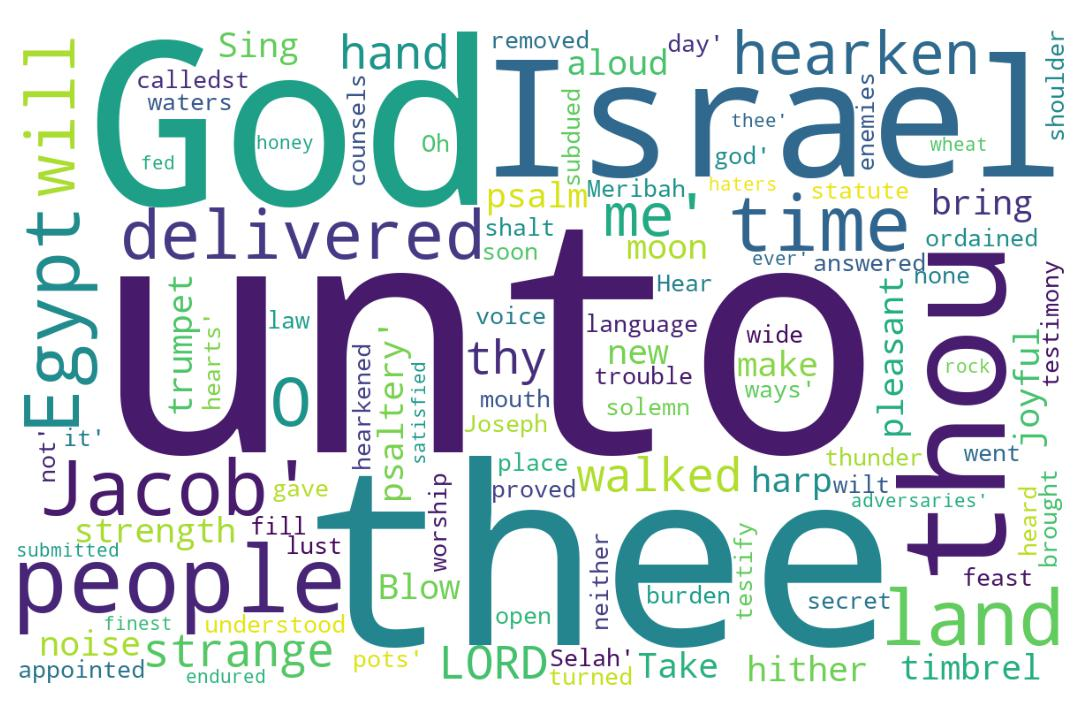
\includegraphics[width=\linewidth]{19OT-Psalms/Psalm81-WordCloud.jpg}
  \caption{Psalm 81 Word Cloud}
  \label{fig:Psalm 81 word Cloud}
\end{figure}



\marginpar{\scriptsize \centering \fcolorbox{bone}{lime}{\textbf{RECOGNIZING ONE'S PLACE}}\\ (Psalm 81) \begin{compactenum}[I.][8]
    \item A \textbf{Call to Rejoice} \index[scripture]{Psalms!Psa 081:01-05}(Psa 81:1-5)
    \item A \textbf{Call to Remember} \index[scripture]{Psalms!Psa 081:06-10}(Psa 81:6-10)
    \item A \textbf{Chains Removed} \index[scripture]{Psalms!Psa 081:06}(Psa 81:6)
    \item The \textbf{Call to be Rescued} \index[scripture]{Psalms!Psa 081:07}(Psa 81:7)
    \item A \textbf{Challenge to Regard God} \index[scripture]{Psalms!Psa 081:08}(Psa 81:8)
    \item A \textbf{Call to Repent} \index[scripture]{Psalms!Psa 081:11-16}(Psa 81:11-16)
\end{compactenum}}




\footnote{\textcolor[rgb]{0.00,0.25,0.00}{\hyperlink{PsalmsTOC}{Return to end of Table of Contents.}}}\footnote{\href{https://audiobible.com/bible/psalms_81.html}{\textcolor[cmyk]{0.99998,1,0,0}{Psalm 81 Audio}}}\textcolor[cmyk]{0.99998,1,0,0}{To the chief Musician upon Gittith, \emph{A Psalm} of Asaph.}\\
\\
\textcolor[cmyk]{0.99998,1,0,0}{Sing aloud unto God our strength: make a joyful noise unto the God of Jacob.} %\footnote{[RUCKMAN]  The first seven verses deal with Israel praising God in its feasts for deliverance from Egypt. The speaker switches from the third person to the first person in the most distracting fashion (vs. 5), where God Himself becomes the speaker in verses 6 and 7. The Psalmist speaks for Israel as “I” in verse 5 (“I heard a language that I understood not”), but immediately places Israel into the second person (“Thou calledst in trouble”), and then speaks for God as “I” (“I delivered thee; I answered thee”). The only other way out is to claim that the “I” of “I heard a language that I understood not” matches Hosea 8:4 and Amos 3:2. It is possible for God to speak of not knowing something that happens right in front of His face. Observe: “I never knew you: depart from me” (Matt. 7:23). Obviously God knows every man’s birth, life, death, thoughts, background, feelings, words, ideas, imaginations, motives, works, and beliefs; but still: “I never knew you.” Thus “I heard a language that I understood not” (vs. 5). However, the former meaning is probably correct; very often a prophet will switch persons. \cite{Ruckman1992Psalms}  }
[2] \textcolor[cmyk]{0.99998,1,0,0}{Take a psalm, and bring hither the timbrel, the pleasant harp with the psaltery.}
[3] \textcolor[cmyk]{0.99998,1,0,0}{Blow up the trumpet in the new moon, in the time appointed, on our solemn feast day.} %\footnote{[RUCKMAN] The “solemn feast day” (vs. 3) is the date of the Second Advent. This date is the Feast of Tabernacles (see 2 Chron. 7:9; Neh. 8:18; Hosea 9:5, 12:9; Lev. 23:34; Deut. 16:13; 31:10; 2 Chron. 8:13; and Ezra 3:4). This is THE outstanding date on the calendar of history from 4000 B.C. to A.D. 2000, for it dates BOTH ADVENTS and is commemorated once a year by the sun itself, which is four days off center from the earth’s orbit; these days are September 20, 21, 22, and 23. The “statute” and “law” that was “ordained” (vss. 4--5) was to confirm the appearance of Jesus Christ after the Marriage of the Lamb (see comments under Ps. 19:4--5). All the commentators....etc., etc. \cite{Ruckman1992Psalms} }
[4] \textcolor[cmyk]{0.99998,1,0,0}{For this \emph{was} a statute for Israel, \emph{and} a law of the God of Jacob.}
[5] \textcolor[cmyk]{0.99998,1,0,0}{This he ordained in Joseph \emph{for} a testimony, when he went out through the land of Egypt: \emph{where} I heard a language \emph{that} I understood not.}
[6] \textcolor[cmyk]{0.99998,1,0,0}{I removed his shoulder from the burden: his hands were delivered from the pots.}
[7] \textcolor[cmyk]{0.99998,1,0,0}{Thou calledst in trouble, and I delivered thee; I answered thee in the secret place of thunder: I proved thee at the waters of Meribah. Selah.} %\footnote{[RUCKMAN]  Verse 7 was an answer to Psalm 50:15. “The secret place of thunder” would be Mt. Sinai (see Exodus 19:16 and 20:18), although the thing will be repeated in the Tribulation (1 Samuel 2:10). You say, “Where do you get THAT from?” That’s easy—“Selah” (vs. 7), right in front of the noses of the Scholar’s Union. You know what they did with it, and you don’t have to be told. Revelation 10:3 and 16:18 are not in the Book to be ignored. The rebuke that God gives Israel, here, was prefaced by verse 7, which said, “I proved thee at the waters of Meribah.” This was Israel’s sin (see Exod. 17:3–7), and it is described in much detail in our Bible Believer’s Commentary on Exodus. “Hear, O my people” (vs. 8), as in 78:1. Nothing that follows is difficult. It was discussed in The Bible Believer’s Commentary on Exodus, which see. \cite{Ruckman1992Psalms} }
[8] \textcolor[cmyk]{0.99998,1,0,0}{Hear, O my people, and I will testify unto thee: O Israel, if thou wilt hearken unto me;}
[9] \textcolor[cmyk]{0.99998,1,0,0}{There shall no strange god be in thee; neither shalt thou worship any strange god.}
[10] \textcolor[cmyk]{0.99998,1,0,0}{I \emph{am} the LORD thy God, which brought thee out of the land of Egypt: open thy mouth wide, and I will fill it.} %\footnote{God will fill their mouths (vs. 10) as a mother eagle will fill the mouth of an offspring, for He brought them out ``on eagles’ wings'' (Exod. 19:4).}
[11] \textcolor[cmyk]{0.99998,1,0,0}{But my people would not hearken to my voice; and Israel would none of me.}
[12] \textcolor[cmyk]{0.99998,1,0,0}{So I gave them up unto their own hearts' lust: \emph{and} they walked in their own counsels.}
[13] \textcolor[cmyk]{0.99998,1,0,0}{Oh that my people had hearkened unto me, \emph{and} Israel had walked in my ways!}
[14] \textcolor[cmyk]{0.99998,1,0,0}{I should soon have subdued their enemies, and turned my hand against their adversaries.}
[15] \textcolor[cmyk]{0.99998,1,0,0}{The haters of the LORD should have submitted themselves unto him: but their time should have endured for ever.}
[16] \textcolor[cmyk]{0.99998,1,0,0}{He should have fed them also with the finest of the wheat: and with honey out of the rock should I have satisfied thee.} %\footnote{Observe the apparent contradiction between verse 16 and Deuteronomy 32:13. One verse said that God did feed them with those items, and the other said He would have if they had obeyed Him. Jamieson, Fausset, Brown, and Kroll find the reference in Deuteronomy, but not knowing what on earth either passage is about, they pretend that there isn’t any problem. Now God testifies against His people. His complaint is the same complaint voiced by Joshua when Israel entered the Promised Land (Josh. 24:14, 19). It is the same complaint and warning that God gave them before they left the wilderness. Turning a deaf ear to this warning is the thing that caused both Israel (2 Kings 18) and Judah (Jer. 39–- 40) to go into captivity: “there shall no strange god be in thee” (vs. 9). God “gave them up” (vs. 12) like He gave up the Gentiles in Romans 1:24–25. Stephen describes this very thing in Acts 7:42. The “they” and “their” in the passage (vss. 12, 14) is Israel, but the “them” of verse 16 is in contrast with the “thee” of verse 16.  This produces a strange thing among the commentators. “Their time” is given to God’s enemies in the NIV and the RSV, but the same expression is attributed to Israel by Jamieson, Fausset, Brown, and Spurgeon. (Kroll wisely keeps his mouth shut so no one will spot his ignorance: Prov. 17:28). The ASV leaves the text as it stands in the AV, but the NKJV (Curtis Hutson, Harold Okenga, James Price, F. F. Bruce, et al.) goes along with the RSV of the National Council of Churches and writes “their fate,” without identifying WHOSE fate. The Living Bible says it is the enemy’s fate, and so do the RSV, NRSV, and NIV. But they could have changed  it. They would have “submitted themselves unto” the Lord. If they had done this, then they would have fed on what Israel fed on in Deuteronomy 32:13. The enemies would not have just been “subdued” (vs. 14), they would have “submitted” themselves to God and Israel, so they would have shared in Israel’s physical and material blessings. Note the Holy Spirit’s comments on this in Romans 11:12, which all the...you know by now! “He should have fed them”—the enemies that God subdued and came into submission —with the things that He fed Israel (see vs. 10). “He should have fed them also” clinches the case. Of course, we can find all kinds of spiritual truths in the Psalm.
%\begin{compactenum}
%\item We got saved when we were “in trouble,” and at that time we called upon the name of the Lord (vs. 7). 
%\item Testings followed our salvation (vs. 7).
%\item From that point on, we were to listen to God, not to man (vs. 8), and since “covetousness...is idolatry” (Col. 3:5), we were to have no “strange gods” (vs. 9).
%\item God will provide FOOD (vs. 10 with 1 Tim. 6:8).
%\item God will fight for us if we yield to Him (vss. 13--14).
%\item Conversions will follow our obedience (vs. 15).
%\item And the converted enemies of God (see Rom. 5:10) would enjoy “honey out of the rock” (see 1 Pet. 2:3).
%\end{compactenum} }


\index[NWIV]{15!Psalms!Psa 81:1}\index[AWIP]{Sing!Psalms!Psa 81:1}\index[AWIP]{aloud!Psalms!Psa 81:1}\index[AWIP]{unto!Psalms!Psa 81:1}\index[AWIP]{unto!Psalms!Psa 81:1 (2)}\index[AWIP]{God!Psalms!Psa 81:1}\index[AWIP]{God!Psalms!Psa 81:1 (2)}\index[AWIP]{our!Psalms!Psa 81:1}\index[AWIP]{strength!Psalms!Psa 81:1}\index[AWIP]{make!Psalms!Psa 81:1}\index[AWIP]{a!Psalms!Psa 81:1}\index[AWIP]{joyful!Psalms!Psa 81:1}\index[AWIP]{noise!Psalms!Psa 81:1}\index[AWIP]{the!Psalms!Psa 81:1}\index[AWIP]{of!Psalms!Psa 81:1}\index[AWIP]{Jacob!Psalms!Psa 81:1}

\index[NWIV]{14!Psalms!Psa 81:2}\index[AWIP]{Take!Psalms!Psa 81:2}\index[AWIP]{a!Psalms!Psa 81:2}\index[AWIP]{psalm!Psalms!Psa 81:2}\index[AWIP]{and!Psalms!Psa 81:2}\index[AWIP]{bring!Psalms!Psa 81:2}\index[AWIP]{hither!Psalms!Psa 81:2}\index[AWIP]{the!Psalms!Psa 81:2}\index[AWIP]{the!Psalms!Psa 81:2 (2)}\index[AWIP]{the!Psalms!Psa 81:2 (3)}\index[AWIP]{timbrel!Psalms!Psa 81:2}\index[AWIP]{pleasant!Psalms!Psa 81:2}\index[AWIP]{harp!Psalms!Psa 81:2}\index[AWIP]{with!Psalms!Psa 81:2}\index[AWIP]{psaltery!Psalms!Psa 81:2}

\index[NWIV]{17!Psalms!Psa 81:3}\index[AWIP]{Blow!Psalms!Psa 81:3}\index[AWIP]{up!Psalms!Psa 81:3}\index[AWIP]{the!Psalms!Psa 81:3}\index[AWIP]{the!Psalms!Psa 81:3 (2)}\index[AWIP]{the!Psalms!Psa 81:3 (3)}\index[AWIP]{trumpet!Psalms!Psa 81:3}\index[AWIP]{in!Psalms!Psa 81:3}\index[AWIP]{in!Psalms!Psa 81:3 (2)}\index[AWIP]{new!Psalms!Psa 81:3}\index[AWIP]{moon!Psalms!Psa 81:3}\index[AWIP]{time!Psalms!Psa 81:3}\index[AWIP]{appointed!Psalms!Psa 81:3}\index[AWIP]{on!Psalms!Psa 81:3}\index[AWIP]{our!Psalms!Psa 81:3}\index[AWIP]{solemn!Psalms!Psa 81:3}\index[AWIP]{feast!Psalms!Psa 81:3}\index[AWIP]{day!Psalms!Psa 81:3}

\index[NWIV]{15!Psalms!Psa 81:4}\index[AWIP]{For!Psalms!Psa 81:4}\index[AWIP]{this!Psalms!Psa 81:4}\index[AWIP]{\emph{was}!Psalms!Psa 81:4}\index[AWIP]{a!Psalms!Psa 81:4}\index[AWIP]{a!Psalms!Psa 81:4 (2)}\index[AWIP]{statute!Psalms!Psa 81:4}\index[AWIP]{for!Psalms!Psa 81:4}\index[AWIP]{Israel!Psalms!Psa 81:4}\index[AWIP]{\emph{and}!Psalms!Psa 81:4}\index[AWIP]{law!Psalms!Psa 81:4}\index[AWIP]{of!Psalms!Psa 81:4}\index[AWIP]{of!Psalms!Psa 81:4 (2)}\index[AWIP]{the!Psalms!Psa 81:4}\index[AWIP]{God!Psalms!Psa 81:4}\index[AWIP]{Jacob!Psalms!Psa 81:4}\index[AWIP]{\emph{was}!Psalms!Psa 81:4}\index[AWIP]{\emph{and}!Psalms!Psa 81:4}

\index[NWIV]{26!Psalms!Psa 81:5}\index[AWIP]{This!Psalms!Psa 81:5}\index[AWIP]{he!Psalms!Psa 81:5}\index[AWIP]{he!Psalms!Psa 81:5 (2)}\index[AWIP]{ordained!Psalms!Psa 81:5}\index[AWIP]{in!Psalms!Psa 81:5}\index[AWIP]{Joseph!Psalms!Psa 81:5}\index[AWIP]{\emph{for}!Psalms!Psa 81:5}\index[AWIP]{a!Psalms!Psa 81:5}\index[AWIP]{a!Psalms!Psa 81:5 (2)}\index[AWIP]{testimony!Psalms!Psa 81:5}\index[AWIP]{when!Psalms!Psa 81:5}\index[AWIP]{went!Psalms!Psa 81:5}\index[AWIP]{out!Psalms!Psa 81:5}\index[AWIP]{through!Psalms!Psa 81:5}\index[AWIP]{the!Psalms!Psa 81:5}\index[AWIP]{land!Psalms!Psa 81:5}\index[AWIP]{of!Psalms!Psa 81:5}\index[AWIP]{Egypt!Psalms!Psa 81:5}\index[AWIP]{\emph{where}!Psalms!Psa 81:5}\index[AWIP]{I!Psalms!Psa 81:5}\index[AWIP]{I!Psalms!Psa 81:5 (2)}\index[AWIP]{heard!Psalms!Psa 81:5}\index[AWIP]{language!Psalms!Psa 81:5}\index[AWIP]{\emph{that}!Psalms!Psa 81:5}\index[AWIP]{understood!Psalms!Psa 81:5}\index[AWIP]{not!Psalms!Psa 81:5}\index[AWIP]{\emph{for}!Psalms!Psa 81:5}\index[AWIP]{\emph{where}!Psalms!Psa 81:5}\index[AWIP]{\emph{that}!Psalms!Psa 81:5}

\index[NWIV]{14!Psalms!Psa 81:6}\index[AWIP]{I!Psalms!Psa 81:6}\index[AWIP]{removed!Psalms!Psa 81:6}\index[AWIP]{his!Psalms!Psa 81:6}\index[AWIP]{his!Psalms!Psa 81:6 (2)}\index[AWIP]{shoulder!Psalms!Psa 81:6}\index[AWIP]{from!Psalms!Psa 81:6}\index[AWIP]{from!Psalms!Psa 81:6 (2)}\index[AWIP]{the!Psalms!Psa 81:6}\index[AWIP]{the!Psalms!Psa 81:6 (2)}\index[AWIP]{burden!Psalms!Psa 81:6}\index[AWIP]{hands!Psalms!Psa 81:6}\index[AWIP]{were!Psalms!Psa 81:6}\index[AWIP]{delivered!Psalms!Psa 81:6}\index[AWIP]{pots!Psalms!Psa 81:6}

\index[NWIV]{26!Psalms!Psa 81:7}\index[AWIP]{Thou!Psalms!Psa 81:7}\index[AWIP]{calledst!Psalms!Psa 81:7}\index[AWIP]{in!Psalms!Psa 81:7}\index[AWIP]{in!Psalms!Psa 81:7 (2)}\index[AWIP]{trouble!Psalms!Psa 81:7}\index[AWIP]{and!Psalms!Psa 81:7}\index[AWIP]{I!Psalms!Psa 81:7}\index[AWIP]{I!Psalms!Psa 81:7 (2)}\index[AWIP]{I!Psalms!Psa 81:7 (3)}\index[AWIP]{delivered!Psalms!Psa 81:7}\index[AWIP]{thee!Psalms!Psa 81:7}\index[AWIP]{thee!Psalms!Psa 81:7 (2)}\index[AWIP]{thee!Psalms!Psa 81:7 (3)}\index[AWIP]{answered!Psalms!Psa 81:7}\index[AWIP]{the!Psalms!Psa 81:7}\index[AWIP]{the!Psalms!Psa 81:7 (2)}\index[AWIP]{secret!Psalms!Psa 81:7}\index[AWIP]{place!Psalms!Psa 81:7}\index[AWIP]{of!Psalms!Psa 81:7}\index[AWIP]{of!Psalms!Psa 81:7 (2)}\index[AWIP]{thunder!Psalms!Psa 81:7}\index[AWIP]{proved!Psalms!Psa 81:7}\index[AWIP]{at!Psalms!Psa 81:7}\index[AWIP]{waters!Psalms!Psa 81:7}\index[AWIP]{Meribah!Psalms!Psa 81:7}\index[AWIP]{Selah!Psalms!Psa 81:7}

\index[NWIV]{18!Psalms!Psa 81:8}\index[AWIP]{Hear!Psalms!Psa 81:8}\index[AWIP]{O!Psalms!Psa 81:8}\index[AWIP]{O!Psalms!Psa 81:8 (2)}\index[AWIP]{my!Psalms!Psa 81:8}\index[AWIP]{people!Psalms!Psa 81:8}\index[AWIP]{and!Psalms!Psa 81:8}\index[AWIP]{I!Psalms!Psa 81:8}\index[AWIP]{will!Psalms!Psa 81:8}\index[AWIP]{testify!Psalms!Psa 81:8}\index[AWIP]{unto!Psalms!Psa 81:8}\index[AWIP]{unto!Psalms!Psa 81:8 (2)}\index[AWIP]{thee!Psalms!Psa 81:8}\index[AWIP]{Israel!Psalms!Psa 81:8}\index[AWIP]{if!Psalms!Psa 81:8}\index[AWIP]{thou!Psalms!Psa 81:8}\index[AWIP]{wilt!Psalms!Psa 81:8}\index[AWIP]{hearken!Psalms!Psa 81:8}\index[AWIP]{me!Psalms!Psa 81:8}

\index[NWIV]{15!Psalms!Psa 81:9}\index[AWIP]{There!Psalms!Psa 81:9}\index[AWIP]{shall!Psalms!Psa 81:9}\index[AWIP]{no!Psalms!Psa 81:9}\index[AWIP]{strange!Psalms!Psa 81:9}\index[AWIP]{strange!Psalms!Psa 81:9 (2)}\index[AWIP]{god!Psalms!Psa 81:9}\index[AWIP]{god!Psalms!Psa 81:9 (2)}\index[AWIP]{be!Psalms!Psa 81:9}\index[AWIP]{in!Psalms!Psa 81:9}\index[AWIP]{thee!Psalms!Psa 81:9}\index[AWIP]{neither!Psalms!Psa 81:9}\index[AWIP]{shalt!Psalms!Psa 81:9}\index[AWIP]{thou!Psalms!Psa 81:9}\index[AWIP]{worship!Psalms!Psa 81:9}\index[AWIP]{any!Psalms!Psa 81:9}

\index[NWIV]{24!Psalms!Psa 81:10}\index[AWIP]{I!Psalms!Psa 81:10}\index[AWIP]{I!Psalms!Psa 81:10 (2)}\index[AWIP]{\emph{am}!Psalms!Psa 81:10}\index[AWIP]{the!Psalms!Psa 81:10}\index[AWIP]{the!Psalms!Psa 81:10 (2)}\index[AWIP]{LORD!Psalms!Psa 81:10}\index[AWIP]{thy!Psalms!Psa 81:10}\index[AWIP]{thy!Psalms!Psa 81:10 (2)}\index[AWIP]{God!Psalms!Psa 81:10}\index[AWIP]{which!Psalms!Psa 81:10}\index[AWIP]{brought!Psalms!Psa 81:10}\index[AWIP]{thee!Psalms!Psa 81:10}\index[AWIP]{out!Psalms!Psa 81:10}\index[AWIP]{of!Psalms!Psa 81:10}\index[AWIP]{of!Psalms!Psa 81:10 (2)}\index[AWIP]{land!Psalms!Psa 81:10}\index[AWIP]{Egypt!Psalms!Psa 81:10}\index[AWIP]{open!Psalms!Psa 81:10}\index[AWIP]{mouth!Psalms!Psa 81:10}\index[AWIP]{wide!Psalms!Psa 81:10}\index[AWIP]{and!Psalms!Psa 81:10}\index[AWIP]{will!Psalms!Psa 81:10}\index[AWIP]{fill!Psalms!Psa 81:10}\index[AWIP]{it!Psalms!Psa 81:10}\index[AWIP]{\emph{am}!Psalms!Psa 81:10}

\index[NWIV]{15!Psalms!Psa 81:11}\index[AWIP]{But!Psalms!Psa 81:11}\index[AWIP]{my!Psalms!Psa 81:11}\index[AWIP]{my!Psalms!Psa 81:11 (2)}\index[AWIP]{people!Psalms!Psa 81:11}\index[AWIP]{would!Psalms!Psa 81:11}\index[AWIP]{would!Psalms!Psa 81:11 (2)}\index[AWIP]{not!Psalms!Psa 81:11}\index[AWIP]{hearken!Psalms!Psa 81:11}\index[AWIP]{to!Psalms!Psa 81:11}\index[AWIP]{voice!Psalms!Psa 81:11}\index[AWIP]{and!Psalms!Psa 81:11}\index[AWIP]{Israel!Psalms!Psa 81:11}\index[AWIP]{none!Psalms!Psa 81:11}\index[AWIP]{of!Psalms!Psa 81:11}\index[AWIP]{me!Psalms!Psa 81:11}

\index[NWIV]{17!Psalms!Psa 81:12}\index[AWIP]{So!Psalms!Psa 81:12}\index[AWIP]{I!Psalms!Psa 81:12}\index[AWIP]{gave!Psalms!Psa 81:12}\index[AWIP]{them!Psalms!Psa 81:12}\index[AWIP]{up!Psalms!Psa 81:12}\index[AWIP]{unto!Psalms!Psa 81:12}\index[AWIP]{their!Psalms!Psa 81:12}\index[AWIP]{their!Psalms!Psa 81:12 (2)}\index[AWIP]{own!Psalms!Psa 81:12}\index[AWIP]{own!Psalms!Psa 81:12 (2)}\index[AWIP]{hearts'!Psalms!Psa 81:12}\index[AWIP]{lust!Psalms!Psa 81:12}\index[AWIP]{\emph{and}!Psalms!Psa 81:12}\index[AWIP]{they!Psalms!Psa 81:12}\index[AWIP]{walked!Psalms!Psa 81:12}\index[AWIP]{in!Psalms!Psa 81:12}\index[AWIP]{counsels!Psalms!Psa 81:12}\index[AWIP]{\emph{and}!Psalms!Psa 81:12}

\index[NWIV]{15!Psalms!Psa 81:13}\index[AWIP]{Oh!Psalms!Psa 81:13}\index[AWIP]{that!Psalms!Psa 81:13}\index[AWIP]{my!Psalms!Psa 81:13}\index[AWIP]{my!Psalms!Psa 81:13 (2)}\index[AWIP]{people!Psalms!Psa 81:13}\index[AWIP]{had!Psalms!Psa 81:13}\index[AWIP]{had!Psalms!Psa 81:13 (2)}\index[AWIP]{hearkened!Psalms!Psa 81:13}\index[AWIP]{unto!Psalms!Psa 81:13}\index[AWIP]{me!Psalms!Psa 81:13}\index[AWIP]{\emph{and}!Psalms!Psa 81:13}\index[AWIP]{Israel!Psalms!Psa 81:13}\index[AWIP]{walked!Psalms!Psa 81:13}\index[AWIP]{in!Psalms!Psa 81:13}\index[AWIP]{ways!!Psalms!Psa 81:13}\index[AWIP]{\emph{and}!Psalms!Psa 81:13}

\index[NWIV]{14!Psalms!Psa 81:14}\index[AWIP]{I!Psalms!Psa 81:14}\index[AWIP]{should!Psalms!Psa 81:14}\index[AWIP]{soon!Psalms!Psa 81:14}\index[AWIP]{have!Psalms!Psa 81:14}\index[AWIP]{subdued!Psalms!Psa 81:14}\index[AWIP]{their!Psalms!Psa 81:14}\index[AWIP]{their!Psalms!Psa 81:14 (2)}\index[AWIP]{enemies!Psalms!Psa 81:14}\index[AWIP]{and!Psalms!Psa 81:14}\index[AWIP]{turned!Psalms!Psa 81:14}\index[AWIP]{my!Psalms!Psa 81:14}\index[AWIP]{hand!Psalms!Psa 81:14}\index[AWIP]{against!Psalms!Psa 81:14}\index[AWIP]{adversaries!Psalms!Psa 81:14}

\index[NWIV]{19!Psalms!Psa 81:15}\index[AWIP]{The!Psalms!Psa 81:15}\index[AWIP]{haters!Psalms!Psa 81:15}\index[AWIP]{of!Psalms!Psa 81:15}\index[AWIP]{the!Psalms!Psa 81:15}\index[AWIP]{LORD!Psalms!Psa 81:15}\index[AWIP]{should!Psalms!Psa 81:15}\index[AWIP]{should!Psalms!Psa 81:15 (2)}\index[AWIP]{have!Psalms!Psa 81:15}\index[AWIP]{have!Psalms!Psa 81:15 (2)}\index[AWIP]{submitted!Psalms!Psa 81:15}\index[AWIP]{themselves!Psalms!Psa 81:15}\index[AWIP]{unto!Psalms!Psa 81:15}\index[AWIP]{him!Psalms!Psa 81:15}\index[AWIP]{but!Psalms!Psa 81:15}\index[AWIP]{their!Psalms!Psa 81:15}\index[AWIP]{time!Psalms!Psa 81:15}\index[AWIP]{endured!Psalms!Psa 81:15}\index[AWIP]{for!Psalms!Psa 81:15}\index[AWIP]{ever!Psalms!Psa 81:15}

\index[NWIV]{24!Psalms!Psa 81:16}\index[AWIP]{He!Psalms!Psa 81:16}\index[AWIP]{should!Psalms!Psa 81:16}\index[AWIP]{should!Psalms!Psa 81:16 (2)}\index[AWIP]{have!Psalms!Psa 81:16}\index[AWIP]{have!Psalms!Psa 81:16 (2)}\index[AWIP]{fed!Psalms!Psa 81:16}\index[AWIP]{them!Psalms!Psa 81:16}\index[AWIP]{also!Psalms!Psa 81:16}\index[AWIP]{with!Psalms!Psa 81:16}\index[AWIP]{with!Psalms!Psa 81:16 (2)}\index[AWIP]{the!Psalms!Psa 81:16}\index[AWIP]{the!Psalms!Psa 81:16 (2)}\index[AWIP]{the!Psalms!Psa 81:16 (3)}\index[AWIP]{finest!Psalms!Psa 81:16}\index[AWIP]{of!Psalms!Psa 81:16}\index[AWIP]{of!Psalms!Psa 81:16 (2)}\index[AWIP]{wheat!Psalms!Psa 81:16}\index[AWIP]{and!Psalms!Psa 81:16}\index[AWIP]{honey!Psalms!Psa 81:16}\index[AWIP]{out!Psalms!Psa 81:16}\index[AWIP]{rock!Psalms!Psa 81:16}\index[AWIP]{I!Psalms!Psa 81:16}\index[AWIP]{satisfied!Psalms!Psa 81:16}\index[AWIP]{thee!Psalms!Psa 81:16}


\section{Psalm 81 Outlines}

\subsection{My Outlines}

\subsubsection{Recognizing One's Place under God}

\index[speaker]{Keith Anthony!Psalm 081 (Recognizing One's Place under God)}
\index[series]{Psalms (Keith Anthony)!Psalm 081 (Recognizing One's Place under God)}
\index[date]{2015/06/04!Psalm 81 (Recognizing One's Place under God) (Keith Anthony)}

\begin{compactenum}[I.]
    \item A \textbf{Call to Rejoice} \index[scripture]{Psalms!Psa 081:01-05}(Psa 81:1-5)
    \item A \textbf{Call to Remember} \index[scripture]{Psalms!Psa 081:06-10}(Psa 81:6-10)
    \item A \textbf{Chains Removed} \index[scripture]{Psalms!Psa 081:06}(Psa 81:6)
    \item The \textbf{Call to be Rescued} \index[scripture]{Psalms!Psa 081:07}(Psa 81:7)
    \item A \textbf{Challenge to Regard God} \index[scripture]{Psalms!Psa 081:08}(Psa 81:8)
    \item A \textbf{Call to Repent} \index[scripture]{Psalms!Psa 081:11-16}(Psa 81:11-16)
\end{compactenum}


\subsection{Outlines from Others}


\section{Psalm 81 Comments}

\subsection{Numeric Nuggets}
There are 13 unique words in verses 1, 4, 9, 11, 13, and 14. The 13$^{th}$ word in the psalm is ``God.''




\subsection{Psalm 81 Repeated Phrases}


%%%%%%%%%%
%%%%%%%%%%
\normalsize
 
\begin{center}
\begin{longtable}{|p{3.0in}|p{0.5in}|}
\caption[Psalm 81 Repeated Phrases]{Psalm 81 Repeated Phrases}\label{table:Repeated Phrases Psalm 81} \\
\hline \multicolumn{1}{|c|}{\textbf{Phrase}} & \multicolumn{1}{c|}{\textbf{Frequency}} \\ \hline 
\endfirsthead
 
\multicolumn{2}{c}
{{\bfseries \tablename\ \thetable{} -- continued from previous page}} \\  
\hline \multicolumn{1}{|c|}{\textbf{Phrase}} & \multicolumn{1}{c|}{\textbf{Frequency}} \\ \hline 
\endhead
 
\hline \multicolumn{2}{c}{{ }} \\ \hline
\endfoot 
of the & 5\\ \hline 
in the & 3\\ \hline 
and I & 3\\ \hline 
my people & 3\\ \hline 
should have & 3\\ \hline 
\end{longtable}
\end{center}



%%%%%%%%%%
%%%%%%%%%%



\section{Psalm 81 Statistics}

%%%%%%%%%%%%%%%%%%%%%%%%%%%
%%%%% Word Statistics
%%%%%%%%%%%%%%%%%%%%%%%%%%


\normalsize



\subsection{Chapter Word Statistics}


%%%%%%%%%%
%%%%%%%%%%
 
\begin{center}
\begin{longtable}{l|c|c|c|c}
\caption[Stats for Psalm 81]{Stats for Psalm 81} \label{table:Stats for Psalm 81} \\ 
\hline \multicolumn{1}{|c|}{\textbf{Verse(s)}} & \multicolumn{1}{|c|}{\textbf{Count}} & \multicolumn{1}{|c|}{\textbf{Unique}} & \multicolumn{1}{|c|}{\textbf{Italics}} & \multicolumn{1}{|c|}{\textbf{Uniq Italic}}  \\ \hline 
\endfirsthead
 
\multicolumn{5}{c}
{{\bfseries \tablename\ \thetable{} -- continued from previous page}} \\  
\hline \multicolumn{1}{|c|}{\textbf{Verse(s)}} & \multicolumn{1}{|c|}{\textbf{Count}} & \multicolumn{1}{|c|}{\textbf{Unique}} & \multicolumn{1}{|c|}{\textbf{Italics}} & \multicolumn{1}{|c|}{\textbf{Uniq Italic}}  \\ \hline 
\endhead
 
\hline \multicolumn{5}{|r|}{{Continued if needed}} \\ \hline
\endfoot 
1 & 15 & 13 & 0 & 0\\ \hline
2 & 14 & 12 & 0 & 0\\ \hline
3 & 17 & 14 & 0 & 0\\ \hline
4 & 15 & 13 & 2 & 2\\ \hline
5 & 26 & 23 & 3 & 3\\ \hline
6 & 14 & 11 & 0 & 0\\ \hline
7 & 26 & 19 & 0 & 0\\ \hline
8 & 18 & 16 & 0 & 0\\ \hline
9 & 15 & 13 & 0 & 0\\ \hline
10 & 24 & 20 & 1 & 1\\ \hline
11 & 15 & 13 & 0 & 0\\ \hline
12 & 17 & 15 & 1 & 1\\ \hline
13 & 15 & 13 & 1 & 1\\ \hline
14 & 14 & 13 & 0 & 0\\ \hline
15 & 19 & 17 & 0 & 0\\ \hline
16 & 24 & 18 & 0 & 0\\ \hline
\hline \hline
Total & 288 & 160 & 8 & 6



\end{longtable}
\end{center}

%%%%%%%%%%
%%%%%%%%%%
 
\subsection{Words by Frequency}

\begin{center}
\begin{longtable}{l|r}
\caption[Word Frequencies in Psalm 81]{Word Frequencies in Psalm 81} \label{table:WordsIn-Psalm-81} \\ 
\hline \multicolumn{1}{|c|}{\textbf{Word}} & \multicolumn{1}{c|}{\textbf{Frequency}} \\ \hline 
\endfirsthead
 
\multicolumn{2}{c}
{{\bfseries \tablename\ \thetable{} -- continued from previous page}} \\ 
\hline \multicolumn{1}{|c|}{\textbf{Word}} & \multicolumn{1}{c|}{\textbf{Frequency}} \\ \hline 
\endhead
 
\hline \multicolumn{2}{|r|}{{Continued if needed}} \\ \hline
\endfoot
 
\hline \hline
\endlastfoot
the & 19 \\ \hline
of & 12 \\ \hline
I & 12 \\ \hline
in & 8 \\ \hline
unto & 7 \\ \hline
and & 7 \\ \hline
thee & 7 \\ \hline
a & 6 \\ \hline
my & 6 \\ \hline
their & 5 \\ \hline
should & 5 \\ \hline
have & 5 \\ \hline
God & 4 \\ \hline
Israel & 4 \\ \hline
with & 3 \\ \hline
\emph{and} & 3 \\ \hline
out & 3 \\ \hline
people & 3 \\ \hline
me & 3 \\ \hline
our & 2 \\ \hline
Jacob & 2 \\ \hline
up & 2 \\ \hline
time & 2 \\ \hline
for & 2 \\ \hline
he & 2 \\ \hline
land & 2 \\ \hline
Egypt & 2 \\ \hline
not & 2 \\ \hline
his & 2 \\ \hline
from & 2 \\ \hline
delivered & 2 \\ \hline
O & 2 \\ \hline
will & 2 \\ \hline
thou & 2 \\ \hline
hearken & 2 \\ \hline
strange & 2 \\ \hline
god & 2 \\ \hline
LORD & 2 \\ \hline
thy & 2 \\ \hline
would & 2 \\ \hline
them & 2 \\ \hline
own & 2 \\ \hline
walked & 2 \\ \hline
had & 2 \\ \hline
Sing & 1 \\ \hline
aloud & 1 \\ \hline
strength & 1 \\ \hline
make & 1 \\ \hline
joyful & 1 \\ \hline
noise & 1 \\ \hline
Take & 1 \\ \hline
psalm & 1 \\ \hline
bring & 1 \\ \hline
hither & 1 \\ \hline
timbrel & 1 \\ \hline
pleasant & 1 \\ \hline
harp & 1 \\ \hline
psaltery & 1 \\ \hline
Blow & 1 \\ \hline
trumpet & 1 \\ \hline
new & 1 \\ \hline
moon & 1 \\ \hline
appointed & 1 \\ \hline
on & 1 \\ \hline
solemn & 1 \\ \hline
feast & 1 \\ \hline
day & 1 \\ \hline
For & 1 \\ \hline
this & 1 \\ \hline
\emph{was} & 1 \\ \hline
statute & 1 \\ \hline
law & 1 \\ \hline
This & 1 \\ \hline
ordained & 1 \\ \hline
Joseph & 1 \\ \hline
\emph{for} & 1 \\ \hline
testimony & 1 \\ \hline
when & 1 \\ \hline
went & 1 \\ \hline
through & 1 \\ \hline
\emph{where} & 1 \\ \hline
heard & 1 \\ \hline
language & 1 \\ \hline
\emph{that} & 1 \\ \hline
understood & 1 \\ \hline
removed & 1 \\ \hline
shoulder & 1 \\ \hline
burden & 1 \\ \hline
hands & 1 \\ \hline
were & 1 \\ \hline
pots & 1 \\ \hline
Thou & 1 \\ \hline
calledst & 1 \\ \hline
trouble & 1 \\ \hline
answered & 1 \\ \hline
secret & 1 \\ \hline
place & 1 \\ \hline
thunder & 1 \\ \hline
proved & 1 \\ \hline
at & 1 \\ \hline
waters & 1 \\ \hline
Meribah & 1 \\ \hline
Selah & 1 \\ \hline
Hear & 1 \\ \hline
testify & 1 \\ \hline
if & 1 \\ \hline
wilt & 1 \\ \hline
There & 1 \\ \hline
shall & 1 \\ \hline
no & 1 \\ \hline
be & 1 \\ \hline
neither & 1 \\ \hline
shalt & 1 \\ \hline
worship & 1 \\ \hline
any & 1 \\ \hline
\emph{am} & 1 \\ \hline
which & 1 \\ \hline
brought & 1 \\ \hline
open & 1 \\ \hline
mouth & 1 \\ \hline
wide & 1 \\ \hline
fill & 1 \\ \hline
it & 1 \\ \hline
But & 1 \\ \hline
to & 1 \\ \hline
voice & 1 \\ \hline
none & 1 \\ \hline
So & 1 \\ \hline
gave & 1 \\ \hline
hearts' & 1 \\ \hline
lust & 1 \\ \hline
they & 1 \\ \hline
counsels & 1 \\ \hline
Oh & 1 \\ \hline
that & 1 \\ \hline
hearkened & 1 \\ \hline
ways & 1 \\ \hline
soon & 1 \\ \hline
subdued & 1 \\ \hline
enemies & 1 \\ \hline
turned & 1 \\ \hline
hand & 1 \\ \hline
against & 1 \\ \hline
adversaries & 1 \\ \hline
The & 1 \\ \hline
haters & 1 \\ \hline
submitted & 1 \\ \hline
themselves & 1 \\ \hline
him & 1 \\ \hline
but & 1 \\ \hline
endured & 1 \\ \hline
ever & 1 \\ \hline
He & 1 \\ \hline
fed & 1 \\ \hline
also & 1 \\ \hline
finest & 1 \\ \hline
wheat & 1 \\ \hline
honey & 1 \\ \hline
rock & 1 \\ \hline
satisfied & 1 \\ \hline
\end{longtable}
\end{center}



\normalsize



\subsection{Words Alphabetically}

\begin{center}
\begin{longtable}{l|r}
\caption[Word Alphabetically in Psalm 81]{Word Alphabetically in Psalm 81} \label{table:WordsIn-Psalm-81} \\ 
\hline \multicolumn{1}{|c|}{\textbf{Word}} & \multicolumn{1}{c|}{\textbf{Frequency}} \\ \hline 
\endfirsthead
 
\multicolumn{2}{c}
{{\bfseries \tablename\ \thetable{} -- continued from previous page}} \\ 
\hline \multicolumn{1}{|c|}{\textbf{Word}} & \multicolumn{1}{c|}{\textbf{Frequency}} \\ \hline 
\endhead
 
\hline \multicolumn{2}{|r|}{{Continued if needed}} \\ \hline
\endfoot
 
\hline \hline
\endlastfoot
Blow & 1 \\ \hline
But & 1 \\ \hline
Egypt & 2 \\ \hline
For & 1 \\ \hline
God & 4 \\ \hline
He & 1 \\ \hline
Hear & 1 \\ \hline
I & 12 \\ \hline
Israel & 4 \\ \hline
Jacob & 2 \\ \hline
Joseph & 1 \\ \hline
LORD & 2 \\ \hline
Meribah & 1 \\ \hline
O & 2 \\ \hline
Oh & 1 \\ \hline
Selah & 1 \\ \hline
Sing & 1 \\ \hline
So & 1 \\ \hline
Take & 1 \\ \hline
The & 1 \\ \hline
There & 1 \\ \hline
This & 1 \\ \hline
Thou & 1 \\ \hline
\emph{am} & 1 \\ \hline
\emph{and} & 3 \\ \hline
\emph{for} & 1 \\ \hline
\emph{that} & 1 \\ \hline
\emph{was} & 1 \\ \hline
\emph{where} & 1 \\ \hline
a & 6 \\ \hline
adversaries & 1 \\ \hline
against & 1 \\ \hline
aloud & 1 \\ \hline
also & 1 \\ \hline
and & 7 \\ \hline
answered & 1 \\ \hline
any & 1 \\ \hline
appointed & 1 \\ \hline
at & 1 \\ \hline
be & 1 \\ \hline
bring & 1 \\ \hline
brought & 1 \\ \hline
burden & 1 \\ \hline
but & 1 \\ \hline
calledst & 1 \\ \hline
counsels & 1 \\ \hline
day & 1 \\ \hline
delivered & 2 \\ \hline
endured & 1 \\ \hline
enemies & 1 \\ \hline
ever & 1 \\ \hline
feast & 1 \\ \hline
fed & 1 \\ \hline
fill & 1 \\ \hline
finest & 1 \\ \hline
for & 2 \\ \hline
from & 2 \\ \hline
gave & 1 \\ \hline
god & 2 \\ \hline
had & 2 \\ \hline
hand & 1 \\ \hline
hands & 1 \\ \hline
harp & 1 \\ \hline
haters & 1 \\ \hline
have & 5 \\ \hline
he & 2 \\ \hline
heard & 1 \\ \hline
hearken & 2 \\ \hline
hearkened & 1 \\ \hline
hearts' & 1 \\ \hline
him & 1 \\ \hline
his & 2 \\ \hline
hither & 1 \\ \hline
honey & 1 \\ \hline
if & 1 \\ \hline
in & 8 \\ \hline
it & 1 \\ \hline
joyful & 1 \\ \hline
land & 2 \\ \hline
language & 1 \\ \hline
law & 1 \\ \hline
lust & 1 \\ \hline
make & 1 \\ \hline
me & 3 \\ \hline
moon & 1 \\ \hline
mouth & 1 \\ \hline
my & 6 \\ \hline
neither & 1 \\ \hline
new & 1 \\ \hline
no & 1 \\ \hline
noise & 1 \\ \hline
none & 1 \\ \hline
not & 2 \\ \hline
of & 12 \\ \hline
on & 1 \\ \hline
open & 1 \\ \hline
ordained & 1 \\ \hline
our & 2 \\ \hline
out & 3 \\ \hline
own & 2 \\ \hline
people & 3 \\ \hline
place & 1 \\ \hline
pleasant & 1 \\ \hline
pots & 1 \\ \hline
proved & 1 \\ \hline
psalm & 1 \\ \hline
psaltery & 1 \\ \hline
removed & 1 \\ \hline
rock & 1 \\ \hline
satisfied & 1 \\ \hline
secret & 1 \\ \hline
shall & 1 \\ \hline
shalt & 1 \\ \hline
should & 5 \\ \hline
shoulder & 1 \\ \hline
solemn & 1 \\ \hline
soon & 1 \\ \hline
statute & 1 \\ \hline
strange & 2 \\ \hline
strength & 1 \\ \hline
subdued & 1 \\ \hline
submitted & 1 \\ \hline
testify & 1 \\ \hline
testimony & 1 \\ \hline
that & 1 \\ \hline
the & 19 \\ \hline
thee & 7 \\ \hline
their & 5 \\ \hline
them & 2 \\ \hline
themselves & 1 \\ \hline
they & 1 \\ \hline
this & 1 \\ \hline
thou & 2 \\ \hline
through & 1 \\ \hline
thunder & 1 \\ \hline
thy & 2 \\ \hline
timbrel & 1 \\ \hline
time & 2 \\ \hline
to & 1 \\ \hline
trouble & 1 \\ \hline
trumpet & 1 \\ \hline
turned & 1 \\ \hline
understood & 1 \\ \hline
unto & 7 \\ \hline
up & 2 \\ \hline
voice & 1 \\ \hline
walked & 2 \\ \hline
waters & 1 \\ \hline
ways & 1 \\ \hline
went & 1 \\ \hline
were & 1 \\ \hline
wheat & 1 \\ \hline
when & 1 \\ \hline
which & 1 \\ \hline
wide & 1 \\ \hline
will & 2 \\ \hline
wilt & 1 \\ \hline
with & 3 \\ \hline
worship & 1 \\ \hline
would & 2 \\ \hline
\end{longtable}
\end{center}



\normalsize



\subsection{Word Lengths in Chapter}
\normalsize
\begin{longtable}{l|p{3.75in}}
\caption[Words by Length in Psalm 81]{Words by Length in Psalm 81} \label{table:WordsIn-Psalm-81} \\ 
\hline \multicolumn{1}{|c|}{\textbf{Length}} & \multicolumn{1}{c|}{\textbf{Words}} \\ \hline 
\endfirsthead
 
\multicolumn{2}{c}
{{\bfseries \tablename\ \thetable{} -- continued from previous page}} \\ 
\hline \multicolumn{1}{|c|}{\textbf{Length}} & \multicolumn{1}{c|}{\textbf{Words}} \\ \hline 
\endhead
 
\hline \multicolumn{2}{|r|}{{Continued if needed}} \\ \hline
\endfoot
 
\hline \hline
\endlastfoot
1 & a, I, O \\ \hline
2 & of, up, in, on, he, at, my, if, me, no, be, \emph{am}, it, to, So, Oh, He \\ \hline
3 & God, our, the, and, new, day, For, \emph{was}, for, \emph{and}, law, \emph{for}, out, not, his, god, any, thy, But, own, had, The, him, but, fed \\ \hline
4 & Sing, unto, make, Take, harp, with, Blow, moon, time, this, This, when, went, land, \emph{that}, from, were, pots, Thou, thee, Hear, will, thou, wilt, LORD, open, wide, fill, none, gave, them, lust, they, that, ways, soon, have, hand, ever, also, rock \\ \hline
5 & aloud, noise, Jacob, psalm, bring, feast, Egypt, \emph{where}, heard, hands, place, Selah, There, shall, shalt, which, mouth, would, voice, their, wheat, honey \\ \hline
6 & joyful, hither, solemn, Israel, Joseph, burden, secret, proved, waters, people, walked, should, turned, haters, finest \\ \hline
7 & timbrel, trumpet, statute, through, removed, trouble, thunder, Meribah, testify, hearken, strange, neither, worship, brought, hearts', subdued, enemies, against, endured \\ \hline
8 & strength, pleasant, psaltery, ordained, language, shoulder, calledst, answered, counsels \\ \hline
9 & appointed, testimony, delivered, hearkened, submitted, satisfied \\ \hline
10 & understood, themselves \\ \hline
11 & adversaries \\ \hline
\end{longtable}






%%%%%%%%%%
%%%%%%%%%%
 



%%%%%%%%%%
%%%%%%%%%%
\subsection{Verses with 18 Words in Chapter}
\normalsize
\begin{longtable}{l|p{3.75in}}
\caption[Verses with 18 Words  in Psalm 81]{Verses with 18 Words  in Psalm 81} \label{table:Verses with 18 Words in-Psalm-81} \\ 
\hline \multicolumn{1}{|c|}{\textbf{Reference}} & \multicolumn{1}{c|}{\textbf{Verse}} \\ \hline 
\endfirsthead
 
\multicolumn{2}{c}
{{\bfseries \tablename\ \thetable{} -- continued from previous page}} \\ 
\hline \multicolumn{1}{|c|}{\textbf{Reference}} & \multicolumn{1}{c|}{\textbf{Verse}} \\ \hline 
\endhead
 
\hline \multicolumn{2}{|r|}{{Continued if needed}} \\ \hline
\endfoot
 
\hline \hline
\endlastfoot
Psalms 081:8 & Hear, O my people, and I will testify unto thee: O Israel, if thou wilt hearken unto me; \\ \hline
\end{longtable}






%%%%%%%%%%
%%%%%%%%%%

\chapter{Proverb 22}

\begin{figure}
  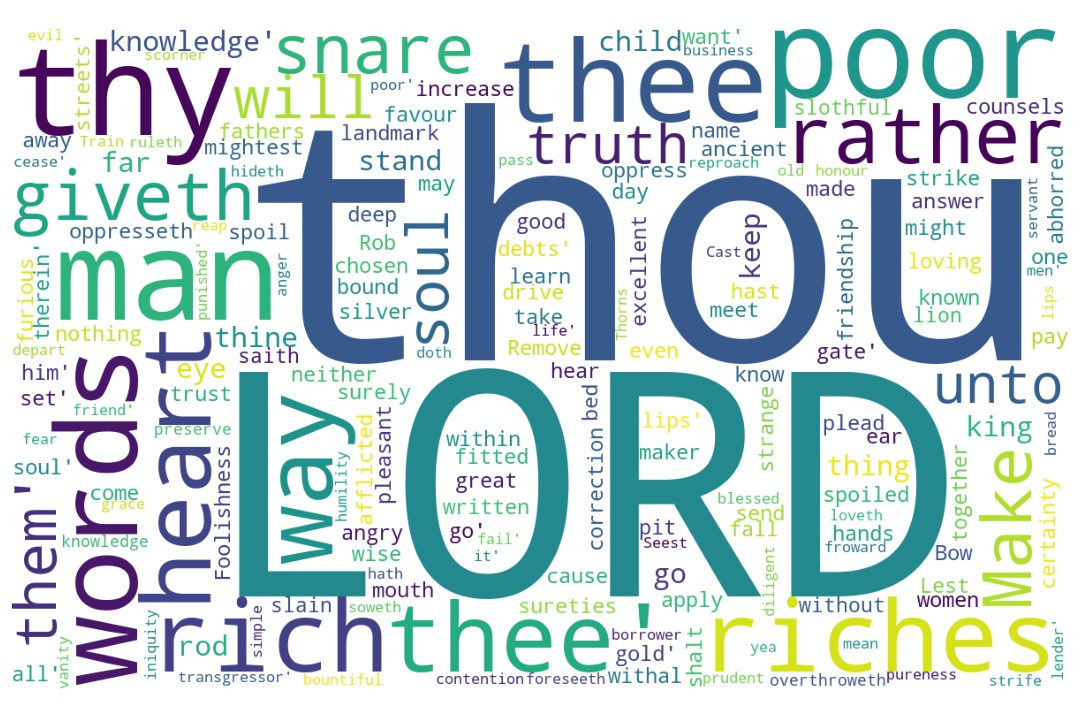
\includegraphics[width=\linewidth]{20OT-Proverbs/Proverb22-WordCloud.jpg}
  \caption{Proverb 22 Word Cloud}
  \label{fig:Proverb 22 word Cloud}
\end{figure}


\marginpar{\scriptsize \centering \fcolorbox{bone}{lime}{\textbf{AN ALL-SEEING GOD}}\\ (Proverb 22:1-29) \begin{compactenum}[I.][8]
    \item \textbf{Are all Around!}(\index[scripture]{Proverbs!Pro 05:21}  \index[scripture]{Proverbs!Pro 15:03}  \index[scripture]{Zechariah!Zch 04:10} (Pro 5:21, Pro 15:3, Zech 4:10)
    \item \textbf{Appraise the Situation} \index[scripture]{1 Kings!1Kng 16:25} \index[scripture]{2 Chronicles!2Chr 14:2}  \index[scripture]{2 Chronicles!2 Chr 21:06}  \index[scripture]{2 Chronicles!2 Chr 29:06} (1Kng 16:25, 2Chr 14:2, 2Chr 21:16, 2Chr 29:6)
    \item \textbf{Are Active} \index[scripture]{Proverbs!Pro 22:12} (Pro 22:12)
    \item \textbf{Approve} \index[scripture]{2 Samuel!2 Sam 15:25} \index[scripture]{Isaiah!Isa 49:05} (2Sam 15:25, Isa 49:5)
    \item \textbf{Are Attentive} (\index[scripture]{Genesis!Gen 6:8}Genesis 06:08, \index[scripture]{2 Chronicles!2 Chr 16:09}2 Chronicles 16:9, \index[scripture]{Psalm!Psa 34:15}Psa 34:15, \index[scripture]{1 Peter!1Pet 03:12}1Pet 3:12)
    \item \textbf{Are Aware} \index[scripture]{Zechariah!Zech 04:10} (Zech 4:10)
    \item \textbf{Analyze} \index[scripture]{Amos!Amo 09:08} (Amos 9:8)
\end{compactenum}}

\marginpar{\scriptsize \centering \fcolorbox{bone}{yellow}{\textbf{SOME ADVICE}}\\ (Proverb 22:1-29) \begin{compactenum}[I.][8]
    \item \textbf{Choice} \index[scripture]{Proverbs!Pro 22:01} (Pro 22:1)
    \item \textbf{Child} \index[scripture]{Proverbs!Pro 22:06}\index[scripture]{Proverbs!Pro 22:15} (Pro 22:6, 15)
    \item \textbf{Contention} \index[scripture]{Proverbs!Pro 22:10} (Pro 22:10)
    \item \textbf{Correction} \index[scripture]{Proverbs!Pro 22:15} (Pro 22:15)
    \item \textbf{Counsels} \index[scripture]{Proverbs!Pro 22:20} (Pro 22:20)
    \item \textbf{Certainty} \index[scripture]{Proverbs!Pro 22:21} (Pro 22:21)
    \item \textbf{Cause} \index[scripture]{Proverbs!Pro 22:23} (Pro 22:23)
\end{compactenum}}

\footnote{\textcolor[cmyk]{0.99998,1,0,0}{\hyperlink{TOC}{Return to end of Table of Contents.}}}\footnote{\href{https://audiobible.com/bible/proverbs_22.html}{\textcolor[cmyk]{0.99998,1,0,0}{Proverbs Audio}}}\textcolor[cmyk]{0.99998,1,0,0}{A \emph{good} name \emph{is} rather to be \fcolorbox{bone}{lime}{chosen} than great riches, \emph{and} loving favour rather than silver and gold.}
[2] \textcolor[cmyk]{0.99998,1,0,0}{The rich and poor meet together: the LORD \emph{is} the maker of them all.}
[3] \textcolor[cmyk]{0.99998,1,0,0}{A prudent \emph{man} foreseeth the evil, and hideth himself: but the simple pass on, and are punished.}
[4] \textcolor[cmyk]{0.99998,1,0,0}{By humility \emph{and} the fear of the LORD \emph{are} riches, and honour, and life.}
[5] \textcolor[cmyk]{0.99998,1,0,0}{Thorns \emph{and} snares \emph{are} in the way of the froward: he that doth keep his soul shall be far from them.}
[6] \textcolor[cmyk]{0.99998,1,0,0}{Train up a \fcolorbox{bone}{lime}{child} in the way he should go: and when he is old, he will not depart from it.}
[7] \textcolor[cmyk]{0.99998,1,0,0}{The rich ruleth over the poor, and the borrower \emph{is} servant to the lender.}
[8] \textcolor[cmyk]{0.99998,1,0,0}{He that soweth iniquity shall reap vanity: and the rod of his anger shall fail.}
[9] \textcolor[cmyk]{0.99998,1,0,0}{He that hath a bountiful eye shall be blessed; for he giveth of his bread to the poor.}\footnote{See Proverbs 21:26 and 14:21. The Roman Vulgate and Alexandrian Septuagint add about eleven to fifteen words not found in the Bible and prove, again, that “Western” and “Alexandrian” manuscripts for the New Testament have the same type of writers, admirers, “preservers,” and believers. For 22:9, the LXX has: ``He that has pity on the poor shall himself be maintained; for he has given of his own bread to the poor. He that gives liberally secures victory an honour; but he takes away the life of them that posses.''}\footnote{\textbf{Proverb 14:21} - He that despiseth his neighbour sinneth: but he that hath mercy on the poor, happy is he.}\footnote{\textbf{Proverb 21:26} - He coveteth greedily all the day long: but the righteous giveth and spareth not.}
[10] \textcolor[cmyk]{0.99998,1,0,0}{Cast out the scorner, and \fcolorbox{bone}{lime}{contention} shall go out; yea, strife and reproach shall cease.}
[11] \textcolor[cmyk]{0.99998,1,0,0}{He that loveth pureness of heart, \emph{for} the grace of his lips the king \emph{shall} \emph{be} his friend.}\footnote{The proverb is clear; especially so in the light of Matthew 5:8 and 2 Samuel 22:27 (see further comment under 21:8). Since God is pure (Hab. 1:13) and the word of God is pure (Psa. 119:140), the “king” (see comments under 20:2, 8 and 21:1) will accept the “pure in heart.” “For the grace of his lips” implies that the pure in heart speaks out of the abundance of his heart (Matt. 5:8). These “lips” are found again in Proverbs 8:6, 10:13, 10:21, 32, 12:19, 14:3, 15:7, and 16:10.}
[12] \textcolor[cmyk]{0.99998,1,0,0}{The eyes of the LORD preserve knowledge, and he overthroweth the words of the transgressor.}
[13] \textcolor[cmyk]{0.99998,1,0,0}{The slothful \emph{man} saith, \emph{There} \emph{is} a lion without, I shall be slain in the streets.}
[14] \textcolor[cmyk]{0.99998,1,0,0}{The mouth of strange women \emph{is} a deep pit: he that is abhorred of the LORD shall fall therein.}
[15] \textcolor[cmyk]{0.99998,1,0,0}{Foolishness \emph{is} bound in the heart of a \fcolorbox{bone}{lime}{child}; \emph{but} the rod of \fcolorbox{bone}{lime}{correction} shall drive it far from him.}
[16] \textcolor[cmyk]{0.99998,1,0,0}{He that oppresseth the poor to increase his \emph{riches,} \emph{and} he that giveth to the rich, \emph{shall} surely \emph{come} to want.}
[17] \textcolor[cmyk]{0.99998,1,0,0}{Bow down thine ear, and hear the words of the wise, and apply thine heart unto my knowledge.}
[18] \textcolor[cmyk]{0.99998,1,0,0}{For \emph{it} \emph{is} a pleasant thing if thou keep them within thee; they shall withal be fitted in thy lips.}
[19] \textcolor[cmyk]{0.99998,1,0,0}{That thy trust may be in the LORD, I have made known to thee this day, even to thee.}
[20] \textcolor[cmyk]{0.99998,1,0,0}{Have not I written to thee excellent things in \fcolorbox{bone}{lime}{counsels} and knowledge,}
[21] \textcolor[cmyk]{0.99998,1,0,0}{That I might make thee know the \fcolorbox{bone}{lime}{certainty} of the words of truth; that thou mightest answer the words of truth to them that send unto thee?}
[22] \textcolor[cmyk]{0.99998,1,0,0}{Rob not the poor, because he \emph{is} poor: neither oppress the afflicted in the gate:}
[23] \textcolor[cmyk]{0.99998,1,0,0}{For the LORD will plead their \fcolorbox{bone}{lime}{cause}, and spoil the soul of those that spoiled them.}
[24] \textcolor[cmyk]{0.99998,1,0,0}{Make no friendship with an angry man; and with a furious man thou shalt not go:}
[25] \textcolor[cmyk]{0.99998,1,0,0}{Lest thou learn his ways, and get a snare to thy soul.}
[26] \textcolor[cmyk]{0.99998,1,0,0}{Be not thou \emph{one} of them that strike hands, \emph{or} of them that are sureties for debts.}
[27] \textcolor[cmyk]{0.99998,1,0,0}{If thou hast nothing to pay, why should he take away thy bed from under thee?}
[28] \textcolor[cmyk]{0.99998,1,0,0}{Remove not the ancient landmark, which thy fathers have set.}\footnote{\textbf{Deuteronomy 19:14} - Thou shalt not remove thy neighbour’s landmark, which they of old time have set in thine inheritance, which thou shalt inherit in the land that the LORD thy God giveth thee to possess it.}\footnote{\textbf{Deuteronomy 27:17} - Cursed be he that removeth his neighbour’s landmark. And all the people shall say, Amen.}\footnote{\textbf{Proverb 23:10} - Remove not the old landmark; and enter not into the fields of the fatherless:}
[29] \textcolor[cmyk]{0.99998,1,0,0}{Seest thou a man diligent in his business? he shall stand before kings; he shall not stand before mean \emph{men}.}\footnote{\textbf{Proverb 21:5} - he thoughts of the diligent tend only to plenteousness; but of every one that is hasty only to want.}\footnote{\textbf{Proverb 27:23} - Be thou diligent to know the state of thy flocks, and look well to thy herds.}\footnote{\textbf{2 Peter 3:14} - Wherefore, beloved, seeing that ye look for such things, be diligent that ye may be found of him in peace, without spot, and blameless.}



\index[NWIV]{19!Proverbs!Pro 22:1}\index[AWIP]{A!Proverbs!Pro 22:1}\index[AWIP]{\emph{good}!Proverbs!Pro 22:1}\index[AWIP]{name!Proverbs!Pro 22:1}\index[AWIP]{\emph{is}!Proverbs!Pro 22:1}\index[AWIP]{rather!Proverbs!Pro 22:1}\index[AWIP]{rather!Proverbs!Pro 22:1 (2)}\index[AWIP]{to!Proverbs!Pro 22:1}\index[AWIP]{be!Proverbs!Pro 22:1}\index[AWIP]{chosen!Proverbs!Pro 22:1}\index[AWIP]{than!Proverbs!Pro 22:1}\index[AWIP]{than!Proverbs!Pro 22:1 (2)}\index[AWIP]{great!Proverbs!Pro 22:1}\index[AWIP]{riches!Proverbs!Pro 22:1}\index[AWIP]{\emph{and}!Proverbs!Pro 22:1}\index[AWIP]{loving!Proverbs!Pro 22:1}\index[AWIP]{favour!Proverbs!Pro 22:1}\index[AWIP]{silver!Proverbs!Pro 22:1}\index[AWIP]{and!Proverbs!Pro 22:1}\index[AWIP]{gold!Proverbs!Pro 22:1}\index[AWIP]{\emph{good}!Proverbs!Pro 22:1}\index[AWIP]{\emph{is}!Proverbs!Pro 22:1}\index[AWIP]{\emph{and}!Proverbs!Pro 22:1}

\index[NWIV]{14!Proverbs!Pro 22:2}\index[AWIP]{The!Proverbs!Pro 22:2}\index[AWIP]{rich!Proverbs!Pro 22:2}\index[AWIP]{and!Proverbs!Pro 22:2}\index[AWIP]{poor!Proverbs!Pro 22:2}\index[AWIP]{meet!Proverbs!Pro 22:2}\index[AWIP]{together!Proverbs!Pro 22:2}\index[AWIP]{the!Proverbs!Pro 22:2}\index[AWIP]{the!Proverbs!Pro 22:2 (2)}\index[AWIP]{LORD!Proverbs!Pro 22:2}\index[AWIP]{\emph{is}!Proverbs!Pro 22:2}\index[AWIP]{maker!Proverbs!Pro 22:2}\index[AWIP]{of!Proverbs!Pro 22:2}\index[AWIP]{them!Proverbs!Pro 22:2}\index[AWIP]{all!Proverbs!Pro 22:2}\index[AWIP]{\emph{is}!Proverbs!Pro 22:2}

\index[NWIV]{17!Proverbs!Pro 22:3}\index[AWIP]{A!Proverbs!Pro 22:3}\index[AWIP]{prudent!Proverbs!Pro 22:3}\index[AWIP]{\emph{man}!Proverbs!Pro 22:3}\index[AWIP]{foreseeth!Proverbs!Pro 22:3}\index[AWIP]{the!Proverbs!Pro 22:3}\index[AWIP]{the!Proverbs!Pro 22:3 (2)}\index[AWIP]{evil!Proverbs!Pro 22:3}\index[AWIP]{and!Proverbs!Pro 22:3}\index[AWIP]{and!Proverbs!Pro 22:3 (2)}\index[AWIP]{hideth!Proverbs!Pro 22:3}\index[AWIP]{himself!Proverbs!Pro 22:3}\index[AWIP]{but!Proverbs!Pro 22:3}\index[AWIP]{simple!Proverbs!Pro 22:3}\index[AWIP]{pass!Proverbs!Pro 22:3}\index[AWIP]{on!Proverbs!Pro 22:3}\index[AWIP]{are!Proverbs!Pro 22:3}\index[AWIP]{punished!Proverbs!Pro 22:3}\index[AWIP]{\emph{man}!Proverbs!Pro 22:3}

\index[NWIV]{14!Proverbs!Pro 22:4}\index[AWIP]{By!Proverbs!Pro 22:4}\index[AWIP]{humility!Proverbs!Pro 22:4}\index[AWIP]{\emph{and}!Proverbs!Pro 22:4}\index[AWIP]{the!Proverbs!Pro 22:4}\index[AWIP]{the!Proverbs!Pro 22:4 (2)}\index[AWIP]{fear!Proverbs!Pro 22:4}\index[AWIP]{of!Proverbs!Pro 22:4}\index[AWIP]{LORD!Proverbs!Pro 22:4}\index[AWIP]{\emph{are}!Proverbs!Pro 22:4}\index[AWIP]{riches!Proverbs!Pro 22:4}\index[AWIP]{and!Proverbs!Pro 22:4}\index[AWIP]{and!Proverbs!Pro 22:4 (2)}\index[AWIP]{honour!Proverbs!Pro 22:4}\index[AWIP]{life!Proverbs!Pro 22:4}\index[AWIP]{\emph{and}!Proverbs!Pro 22:4}\index[AWIP]{\emph{are}!Proverbs!Pro 22:4}

\index[NWIV]{21!Proverbs!Pro 22:5}\index[AWIP]{Thorns!Proverbs!Pro 22:5}\index[AWIP]{\emph{and}!Proverbs!Pro 22:5}\index[AWIP]{snares!Proverbs!Pro 22:5}\index[AWIP]{\emph{are}!Proverbs!Pro 22:5}\index[AWIP]{in!Proverbs!Pro 22:5}\index[AWIP]{the!Proverbs!Pro 22:5}\index[AWIP]{the!Proverbs!Pro 22:5 (2)}\index[AWIP]{way!Proverbs!Pro 22:5}\index[AWIP]{of!Proverbs!Pro 22:5}\index[AWIP]{froward!Proverbs!Pro 22:5}\index[AWIP]{he!Proverbs!Pro 22:5}\index[AWIP]{that!Proverbs!Pro 22:5}\index[AWIP]{doth!Proverbs!Pro 22:5}\index[AWIP]{keep!Proverbs!Pro 22:5}\index[AWIP]{his!Proverbs!Pro 22:5}\index[AWIP]{soul!Proverbs!Pro 22:5}\index[AWIP]{shall!Proverbs!Pro 22:5}\index[AWIP]{be!Proverbs!Pro 22:5}\index[AWIP]{far!Proverbs!Pro 22:5}\index[AWIP]{from!Proverbs!Pro 22:5}\index[AWIP]{them!Proverbs!Pro 22:5}\index[AWIP]{\emph{and}!Proverbs!Pro 22:5}\index[AWIP]{\emph{are}!Proverbs!Pro 22:5}

\index[NWIV]{21!Proverbs!Pro 22:6}\index[AWIP]{Train!Proverbs!Pro 22:6}\index[AWIP]{up!Proverbs!Pro 22:6}\index[AWIP]{a!Proverbs!Pro 22:6}\index[AWIP]{child!Proverbs!Pro 22:6}\index[AWIP]{in!Proverbs!Pro 22:6}\index[AWIP]{the!Proverbs!Pro 22:6}\index[AWIP]{way!Proverbs!Pro 22:6}\index[AWIP]{he!Proverbs!Pro 22:6}\index[AWIP]{he!Proverbs!Pro 22:6 (2)}\index[AWIP]{he!Proverbs!Pro 22:6 (3)}\index[AWIP]{should!Proverbs!Pro 22:6}\index[AWIP]{go!Proverbs!Pro 22:6}\index[AWIP]{and!Proverbs!Pro 22:6}\index[AWIP]{when!Proverbs!Pro 22:6}\index[AWIP]{is!Proverbs!Pro 22:6}\index[AWIP]{old!Proverbs!Pro 22:6}\index[AWIP]{will!Proverbs!Pro 22:6}\index[AWIP]{not!Proverbs!Pro 22:6}\index[AWIP]{depart!Proverbs!Pro 22:6}\index[AWIP]{from!Proverbs!Pro 22:6}\index[AWIP]{it!Proverbs!Pro 22:6}

\index[NWIV]{14!Proverbs!Pro 22:7}\index[AWIP]{The!Proverbs!Pro 22:7}\index[AWIP]{rich!Proverbs!Pro 22:7}\index[AWIP]{ruleth!Proverbs!Pro 22:7}\index[AWIP]{over!Proverbs!Pro 22:7}\index[AWIP]{the!Proverbs!Pro 22:7}\index[AWIP]{the!Proverbs!Pro 22:7 (2)}\index[AWIP]{the!Proverbs!Pro 22:7 (3)}\index[AWIP]{poor!Proverbs!Pro 22:7}\index[AWIP]{and!Proverbs!Pro 22:7}\index[AWIP]{borrower!Proverbs!Pro 22:7}\index[AWIP]{\emph{is}!Proverbs!Pro 22:7}\index[AWIP]{servant!Proverbs!Pro 22:7}\index[AWIP]{to!Proverbs!Pro 22:7}\index[AWIP]{lender!Proverbs!Pro 22:7}\index[AWIP]{\emph{is}!Proverbs!Pro 22:7}

\index[NWIV]{15!Proverbs!Pro 22:8}\index[AWIP]{He!Proverbs!Pro 22:8}\index[AWIP]{that!Proverbs!Pro 22:8}\index[AWIP]{soweth!Proverbs!Pro 22:8}\index[AWIP]{iniquity!Proverbs!Pro 22:8}\index[AWIP]{shall!Proverbs!Pro 22:8}\index[AWIP]{shall!Proverbs!Pro 22:8 (2)}\index[AWIP]{reap!Proverbs!Pro 22:8}\index[AWIP]{vanity!Proverbs!Pro 22:8}\index[AWIP]{and!Proverbs!Pro 22:8}\index[AWIP]{the!Proverbs!Pro 22:8}\index[AWIP]{rod!Proverbs!Pro 22:8}\index[AWIP]{of!Proverbs!Pro 22:8}\index[AWIP]{his!Proverbs!Pro 22:8}\index[AWIP]{anger!Proverbs!Pro 22:8}\index[AWIP]{fail!Proverbs!Pro 22:8}

\index[NWIV]{18!Proverbs!Pro 22:9}\index[AWIP]{He!Proverbs!Pro 22:9}\index[AWIP]{that!Proverbs!Pro 22:9}\index[AWIP]{hath!Proverbs!Pro 22:9}\index[AWIP]{a!Proverbs!Pro 22:9}\index[AWIP]{bountiful!Proverbs!Pro 22:9}\index[AWIP]{eye!Proverbs!Pro 22:9}\index[AWIP]{shall!Proverbs!Pro 22:9}\index[AWIP]{be!Proverbs!Pro 22:9}\index[AWIP]{blessed!Proverbs!Pro 22:9}\index[AWIP]{for!Proverbs!Pro 22:9}\index[AWIP]{he!Proverbs!Pro 22:9}\index[AWIP]{giveth!Proverbs!Pro 22:9}\index[AWIP]{of!Proverbs!Pro 22:9}\index[AWIP]{his!Proverbs!Pro 22:9}\index[AWIP]{bread!Proverbs!Pro 22:9}\index[AWIP]{to!Proverbs!Pro 22:9}\index[AWIP]{the!Proverbs!Pro 22:9}\index[AWIP]{poor!Proverbs!Pro 22:9}

\index[NWIV]{15!Proverbs!Pro 22:10}\index[AWIP]{Cast!Proverbs!Pro 22:10}\index[AWIP]{out!Proverbs!Pro 22:10}\index[AWIP]{out!Proverbs!Pro 22:10 (2)}\index[AWIP]{the!Proverbs!Pro 22:10}\index[AWIP]{scorner!Proverbs!Pro 22:10}\index[AWIP]{and!Proverbs!Pro 22:10}\index[AWIP]{and!Proverbs!Pro 22:10 (2)}\index[AWIP]{contention!Proverbs!Pro 22:10}\index[AWIP]{shall!Proverbs!Pro 22:10}\index[AWIP]{shall!Proverbs!Pro 22:10 (2)}\index[AWIP]{go!Proverbs!Pro 22:10}\index[AWIP]{yea!Proverbs!Pro 22:10}\index[AWIP]{strife!Proverbs!Pro 22:10}\index[AWIP]{reproach!Proverbs!Pro 22:10}\index[AWIP]{cease!Proverbs!Pro 22:10}

\index[NWIV]{18!Proverbs!Pro 22:11}\index[AWIP]{He!Proverbs!Pro 22:11}\index[AWIP]{that!Proverbs!Pro 22:11}\index[AWIP]{loveth!Proverbs!Pro 22:11}\index[AWIP]{pureness!Proverbs!Pro 22:11}\index[AWIP]{of!Proverbs!Pro 22:11}\index[AWIP]{of!Proverbs!Pro 22:11 (2)}\index[AWIP]{heart!Proverbs!Pro 22:11}\index[AWIP]{\emph{for}!Proverbs!Pro 22:11}\index[AWIP]{the!Proverbs!Pro 22:11}\index[AWIP]{the!Proverbs!Pro 22:11 (2)}\index[AWIP]{grace!Proverbs!Pro 22:11}\index[AWIP]{his!Proverbs!Pro 22:11}\index[AWIP]{his!Proverbs!Pro 22:11 (2)}\index[AWIP]{lips!Proverbs!Pro 22:11}\index[AWIP]{king!Proverbs!Pro 22:11}\index[AWIP]{\emph{shall}!Proverbs!Pro 22:11}\index[AWIP]{\emph{be}!Proverbs!Pro 22:11}\index[AWIP]{friend!Proverbs!Pro 22:11}\index[AWIP]{\emph{for}!Proverbs!Pro 22:11}\index[AWIP]{\emph{shall}!Proverbs!Pro 22:11}\index[AWIP]{\emph{be}!Proverbs!Pro 22:11}

\index[NWIV]{15!Proverbs!Pro 22:12}\index[AWIP]{The!Proverbs!Pro 22:12}\index[AWIP]{eyes!Proverbs!Pro 22:12}\index[AWIP]{of!Proverbs!Pro 22:12}\index[AWIP]{of!Proverbs!Pro 22:12 (2)}\index[AWIP]{the!Proverbs!Pro 22:12}\index[AWIP]{the!Proverbs!Pro 22:12 (2)}\index[AWIP]{the!Proverbs!Pro 22:12 (3)}\index[AWIP]{LORD!Proverbs!Pro 22:12}\index[AWIP]{preserve!Proverbs!Pro 22:12}\index[AWIP]{knowledge!Proverbs!Pro 22:12}\index[AWIP]{and!Proverbs!Pro 22:12}\index[AWIP]{he!Proverbs!Pro 22:12}\index[AWIP]{overthroweth!Proverbs!Pro 22:12}\index[AWIP]{words!Proverbs!Pro 22:12}\index[AWIP]{transgressor!Proverbs!Pro 22:12}

\index[NWIV]{16!Proverbs!Pro 22:13}\index[AWIP]{The!Proverbs!Pro 22:13}\index[AWIP]{slothful!Proverbs!Pro 22:13}\index[AWIP]{\emph{man}!Proverbs!Pro 22:13}\index[AWIP]{saith!Proverbs!Pro 22:13}\index[AWIP]{\emph{There}!Proverbs!Pro 22:13}\index[AWIP]{\emph{is}!Proverbs!Pro 22:13}\index[AWIP]{a!Proverbs!Pro 22:13}\index[AWIP]{lion!Proverbs!Pro 22:13}\index[AWIP]{without!Proverbs!Pro 22:13}\index[AWIP]{I!Proverbs!Pro 22:13}\index[AWIP]{shall!Proverbs!Pro 22:13}\index[AWIP]{be!Proverbs!Pro 22:13}\index[AWIP]{slain!Proverbs!Pro 22:13}\index[AWIP]{in!Proverbs!Pro 22:13}\index[AWIP]{the!Proverbs!Pro 22:13}\index[AWIP]{streets!Proverbs!Pro 22:13}\index[AWIP]{\emph{man}!Proverbs!Pro 22:13}\index[AWIP]{\emph{There}!Proverbs!Pro 22:13}\index[AWIP]{\emph{is}!Proverbs!Pro 22:13}

\index[NWIV]{19!Proverbs!Pro 22:14}\index[AWIP]{The!Proverbs!Pro 22:14}\index[AWIP]{mouth!Proverbs!Pro 22:14}\index[AWIP]{of!Proverbs!Pro 22:14}\index[AWIP]{of!Proverbs!Pro 22:14 (2)}\index[AWIP]{strange!Proverbs!Pro 22:14}\index[AWIP]{women!Proverbs!Pro 22:14}\index[AWIP]{\emph{is}!Proverbs!Pro 22:14}\index[AWIP]{a!Proverbs!Pro 22:14}\index[AWIP]{deep!Proverbs!Pro 22:14}\index[AWIP]{pit!Proverbs!Pro 22:14}\index[AWIP]{he!Proverbs!Pro 22:14}\index[AWIP]{that!Proverbs!Pro 22:14}\index[AWIP]{is!Proverbs!Pro 22:14}\index[AWIP]{abhorred!Proverbs!Pro 22:14}\index[AWIP]{the!Proverbs!Pro 22:14}\index[AWIP]{LORD!Proverbs!Pro 22:14}\index[AWIP]{shall!Proverbs!Pro 22:14}\index[AWIP]{fall!Proverbs!Pro 22:14}\index[AWIP]{therein!Proverbs!Pro 22:14}\index[AWIP]{\emph{is}!Proverbs!Pro 22:14}

\index[NWIV]{20!Proverbs!Pro 22:15}\index[AWIP]{Foolishness!Proverbs!Pro 22:15}\index[AWIP]{\emph{is}!Proverbs!Pro 22:15}\index[AWIP]{bound!Proverbs!Pro 22:15}\index[AWIP]{in!Proverbs!Pro 22:15}\index[AWIP]{the!Proverbs!Pro 22:15}\index[AWIP]{the!Proverbs!Pro 22:15 (2)}\index[AWIP]{heart!Proverbs!Pro 22:15}\index[AWIP]{of!Proverbs!Pro 22:15}\index[AWIP]{of!Proverbs!Pro 22:15 (2)}\index[AWIP]{a!Proverbs!Pro 22:15}\index[AWIP]{child!Proverbs!Pro 22:15}\index[AWIP]{\emph{but}!Proverbs!Pro 22:15}\index[AWIP]{rod!Proverbs!Pro 22:15}\index[AWIP]{correction!Proverbs!Pro 22:15}\index[AWIP]{shall!Proverbs!Pro 22:15}\index[AWIP]{drive!Proverbs!Pro 22:15}\index[AWIP]{it!Proverbs!Pro 22:15}\index[AWIP]{far!Proverbs!Pro 22:15}\index[AWIP]{from!Proverbs!Pro 22:15}\index[AWIP]{him!Proverbs!Pro 22:15}\index[AWIP]{\emph{is}!Proverbs!Pro 22:15}\index[AWIP]{\emph{but}!Proverbs!Pro 22:15}

\index[NWIV]{21!Proverbs!Pro 22:16}\index[AWIP]{He!Proverbs!Pro 22:16}\index[AWIP]{that!Proverbs!Pro 22:16}\index[AWIP]{that!Proverbs!Pro 22:16 (2)}\index[AWIP]{oppresseth!Proverbs!Pro 22:16}\index[AWIP]{the!Proverbs!Pro 22:16}\index[AWIP]{the!Proverbs!Pro 22:16 (2)}\index[AWIP]{poor!Proverbs!Pro 22:16}\index[AWIP]{to!Proverbs!Pro 22:16}\index[AWIP]{to!Proverbs!Pro 22:16 (2)}\index[AWIP]{to!Proverbs!Pro 22:16 (3)}\index[AWIP]{increase!Proverbs!Pro 22:16}\index[AWIP]{his!Proverbs!Pro 22:16}\index[AWIP]{\emph{riches}!Proverbs!Pro 22:16}\index[AWIP]{\emph{and}!Proverbs!Pro 22:16}\index[AWIP]{he!Proverbs!Pro 22:16}\index[AWIP]{giveth!Proverbs!Pro 22:16}\index[AWIP]{rich!Proverbs!Pro 22:16}\index[AWIP]{\emph{shall}!Proverbs!Pro 22:16}\index[AWIP]{surely!Proverbs!Pro 22:16}\index[AWIP]{\emph{come}!Proverbs!Pro 22:16}\index[AWIP]{want!Proverbs!Pro 22:16}\index[AWIP]{\emph{riches}!Proverbs!Pro 22:16}\index[AWIP]{\emph{and}!Proverbs!Pro 22:16}\index[AWIP]{\emph{shall}!Proverbs!Pro 22:16}\index[AWIP]{\emph{come}!Proverbs!Pro 22:16}

\index[NWIV]{18!Proverbs!Pro 22:17}\index[AWIP]{Bow!Proverbs!Pro 22:17}\index[AWIP]{down!Proverbs!Pro 22:17}\index[AWIP]{thine!Proverbs!Pro 22:17}\index[AWIP]{thine!Proverbs!Pro 22:17 (2)}\index[AWIP]{ear!Proverbs!Pro 22:17}\index[AWIP]{and!Proverbs!Pro 22:17}\index[AWIP]{and!Proverbs!Pro 22:17 (2)}\index[AWIP]{hear!Proverbs!Pro 22:17}\index[AWIP]{the!Proverbs!Pro 22:17}\index[AWIP]{the!Proverbs!Pro 22:17 (2)}\index[AWIP]{words!Proverbs!Pro 22:17}\index[AWIP]{of!Proverbs!Pro 22:17}\index[AWIP]{wise!Proverbs!Pro 22:17}\index[AWIP]{apply!Proverbs!Pro 22:17}\index[AWIP]{heart!Proverbs!Pro 22:17}\index[AWIP]{unto!Proverbs!Pro 22:17}\index[AWIP]{my!Proverbs!Pro 22:17}\index[AWIP]{knowledge!Proverbs!Pro 22:17}

\index[NWIV]{20!Proverbs!Pro 22:18}\index[AWIP]{For!Proverbs!Pro 22:18}\index[AWIP]{\emph{it}!Proverbs!Pro 22:18}\index[AWIP]{\emph{is}!Proverbs!Pro 22:18}\index[AWIP]{a!Proverbs!Pro 22:18}\index[AWIP]{pleasant!Proverbs!Pro 22:18}\index[AWIP]{thing!Proverbs!Pro 22:18}\index[AWIP]{if!Proverbs!Pro 22:18}\index[AWIP]{thou!Proverbs!Pro 22:18}\index[AWIP]{keep!Proverbs!Pro 22:18}\index[AWIP]{them!Proverbs!Pro 22:18}\index[AWIP]{within!Proverbs!Pro 22:18}\index[AWIP]{thee!Proverbs!Pro 22:18}\index[AWIP]{they!Proverbs!Pro 22:18}\index[AWIP]{shall!Proverbs!Pro 22:18}\index[AWIP]{withal!Proverbs!Pro 22:18}\index[AWIP]{be!Proverbs!Pro 22:18}\index[AWIP]{fitted!Proverbs!Pro 22:18}\index[AWIP]{in!Proverbs!Pro 22:18}\index[AWIP]{thy!Proverbs!Pro 22:18}\index[AWIP]{lips!Proverbs!Pro 22:18}\index[AWIP]{\emph{it}!Proverbs!Pro 22:18}\index[AWIP]{\emph{is}!Proverbs!Pro 22:18}

\index[NWIV]{19!Proverbs!Pro 22:19}\index[AWIP]{That!Proverbs!Pro 22:19}\index[AWIP]{thy!Proverbs!Pro 22:19}\index[AWIP]{trust!Proverbs!Pro 22:19}\index[AWIP]{may!Proverbs!Pro 22:19}\index[AWIP]{be!Proverbs!Pro 22:19}\index[AWIP]{in!Proverbs!Pro 22:19}\index[AWIP]{the!Proverbs!Pro 22:19}\index[AWIP]{LORD!Proverbs!Pro 22:19}\index[AWIP]{I!Proverbs!Pro 22:19}\index[AWIP]{have!Proverbs!Pro 22:19}\index[AWIP]{made!Proverbs!Pro 22:19}\index[AWIP]{known!Proverbs!Pro 22:19}\index[AWIP]{to!Proverbs!Pro 22:19}\index[AWIP]{to!Proverbs!Pro 22:19 (2)}\index[AWIP]{thee!Proverbs!Pro 22:19}\index[AWIP]{thee!Proverbs!Pro 22:19 (2)}\index[AWIP]{this!Proverbs!Pro 22:19}\index[AWIP]{day!Proverbs!Pro 22:19}\index[AWIP]{even!Proverbs!Pro 22:19}

\index[NWIV]{12!Proverbs!Pro 22:20}\index[AWIP]{Have!Proverbs!Pro 22:20}\index[AWIP]{not!Proverbs!Pro 22:20}\index[AWIP]{I!Proverbs!Pro 22:20}\index[AWIP]{written!Proverbs!Pro 22:20}\index[AWIP]{to!Proverbs!Pro 22:20}\index[AWIP]{thee!Proverbs!Pro 22:20}\index[AWIP]{excellent!Proverbs!Pro 22:20}\index[AWIP]{things!Proverbs!Pro 22:20}\index[AWIP]{in!Proverbs!Pro 22:20}\index[AWIP]{counsels!Proverbs!Pro 22:20}\index[AWIP]{and!Proverbs!Pro 22:20}\index[AWIP]{knowledge!Proverbs!Pro 22:20}

\index[NWIV]{27!Proverbs!Pro 22:21}\index[AWIP]{That!Proverbs!Pro 22:21}\index[AWIP]{I!Proverbs!Pro 22:21}\index[AWIP]{might!Proverbs!Pro 22:21}\index[AWIP]{make!Proverbs!Pro 22:21}\index[AWIP]{thee!Proverbs!Pro 22:21}\index[AWIP]{know!Proverbs!Pro 22:21}\index[AWIP]{the!Proverbs!Pro 22:21}\index[AWIP]{the!Proverbs!Pro 22:21 (2)}\index[AWIP]{the!Proverbs!Pro 22:21 (3)}\index[AWIP]{certainty!Proverbs!Pro 22:21}\index[AWIP]{of!Proverbs!Pro 22:21}\index[AWIP]{of!Proverbs!Pro 22:21 (2)}\index[AWIP]{of!Proverbs!Pro 22:21 (3)}\index[AWIP]{words!Proverbs!Pro 22:21}\index[AWIP]{words!Proverbs!Pro 22:21 (2)}\index[AWIP]{truth!Proverbs!Pro 22:21}\index[AWIP]{truth!Proverbs!Pro 22:21 (2)}\index[AWIP]{that!Proverbs!Pro 22:21}\index[AWIP]{that!Proverbs!Pro 22:21 (2)}\index[AWIP]{thou!Proverbs!Pro 22:21}\index[AWIP]{mightest!Proverbs!Pro 22:21}\index[AWIP]{answer!Proverbs!Pro 22:21}\index[AWIP]{to!Proverbs!Pro 22:21}\index[AWIP]{them!Proverbs!Pro 22:21}\index[AWIP]{send!Proverbs!Pro 22:21}\index[AWIP]{unto!Proverbs!Pro 22:21}\index[AWIP]{thee?!Proverbs!Pro 22:21}

\index[NWIV]{15!Proverbs!Pro 22:22}\index[AWIP]{Rob!Proverbs!Pro 22:22}\index[AWIP]{not!Proverbs!Pro 22:22}\index[AWIP]{the!Proverbs!Pro 22:22}\index[AWIP]{the!Proverbs!Pro 22:22 (2)}\index[AWIP]{the!Proverbs!Pro 22:22 (3)}\index[AWIP]{poor!Proverbs!Pro 22:22}\index[AWIP]{poor!Proverbs!Pro 22:22 (2)}\index[AWIP]{because!Proverbs!Pro 22:22}\index[AWIP]{he!Proverbs!Pro 22:22}\index[AWIP]{\emph{is}!Proverbs!Pro 22:22}\index[AWIP]{neither!Proverbs!Pro 22:22}\index[AWIP]{oppress!Proverbs!Pro 22:22}\index[AWIP]{afflicted!Proverbs!Pro 22:22}\index[AWIP]{in!Proverbs!Pro 22:22}\index[AWIP]{gate!Proverbs!Pro 22:22}\index[AWIP]{\emph{is}!Proverbs!Pro 22:22}

\index[NWIV]{16!Proverbs!Pro 22:23}\index[AWIP]{For!Proverbs!Pro 22:23}\index[AWIP]{the!Proverbs!Pro 22:23}\index[AWIP]{the!Proverbs!Pro 22:23 (2)}\index[AWIP]{LORD!Proverbs!Pro 22:23}\index[AWIP]{will!Proverbs!Pro 22:23}\index[AWIP]{plead!Proverbs!Pro 22:23}\index[AWIP]{their!Proverbs!Pro 22:23}\index[AWIP]{cause!Proverbs!Pro 22:23}\index[AWIP]{and!Proverbs!Pro 22:23}\index[AWIP]{spoil!Proverbs!Pro 22:23}\index[AWIP]{soul!Proverbs!Pro 22:23}\index[AWIP]{of!Proverbs!Pro 22:23}\index[AWIP]{those!Proverbs!Pro 22:23}\index[AWIP]{that!Proverbs!Pro 22:23}\index[AWIP]{spoiled!Proverbs!Pro 22:23}\index[AWIP]{them!Proverbs!Pro 22:23}

\index[NWIV]{16!Proverbs!Pro 22:24}\index[AWIP]{Make!Proverbs!Pro 22:24}\index[AWIP]{no!Proverbs!Pro 22:24}\index[AWIP]{friendship!Proverbs!Pro 22:24}\index[AWIP]{with!Proverbs!Pro 22:24}\index[AWIP]{with!Proverbs!Pro 22:24 (2)}\index[AWIP]{an!Proverbs!Pro 22:24}\index[AWIP]{angry!Proverbs!Pro 22:24}\index[AWIP]{man!Proverbs!Pro 22:24}\index[AWIP]{man!Proverbs!Pro 22:24 (2)}\index[AWIP]{and!Proverbs!Pro 22:24}\index[AWIP]{a!Proverbs!Pro 22:24}\index[AWIP]{furious!Proverbs!Pro 22:24}\index[AWIP]{thou!Proverbs!Pro 22:24}\index[AWIP]{shalt!Proverbs!Pro 22:24}\index[AWIP]{not!Proverbs!Pro 22:24}\index[AWIP]{go!Proverbs!Pro 22:24}

\index[NWIV]{12!Proverbs!Pro 22:25}\index[AWIP]{Lest!Proverbs!Pro 22:25}\index[AWIP]{thou!Proverbs!Pro 22:25}\index[AWIP]{learn!Proverbs!Pro 22:25}\index[AWIP]{his!Proverbs!Pro 22:25}\index[AWIP]{ways!Proverbs!Pro 22:25}\index[AWIP]{and!Proverbs!Pro 22:25}\index[AWIP]{get!Proverbs!Pro 22:25}\index[AWIP]{a!Proverbs!Pro 22:25}\index[AWIP]{snare!Proverbs!Pro 22:25}\index[AWIP]{to!Proverbs!Pro 22:25}\index[AWIP]{thy!Proverbs!Pro 22:25}\index[AWIP]{soul!Proverbs!Pro 22:25}

\index[NWIV]{17!Proverbs!Pro 22:26}\index[AWIP]{Be!Proverbs!Pro 22:26}\index[AWIP]{not!Proverbs!Pro 22:26}\index[AWIP]{thou!Proverbs!Pro 22:26}\index[AWIP]{\emph{one}!Proverbs!Pro 22:26}\index[AWIP]{of!Proverbs!Pro 22:26}\index[AWIP]{of!Proverbs!Pro 22:26 (2)}\index[AWIP]{them!Proverbs!Pro 22:26}\index[AWIP]{them!Proverbs!Pro 22:26 (2)}\index[AWIP]{that!Proverbs!Pro 22:26}\index[AWIP]{that!Proverbs!Pro 22:26 (2)}\index[AWIP]{strike!Proverbs!Pro 22:26}\index[AWIP]{hands!Proverbs!Pro 22:26}\index[AWIP]{\emph{or}!Proverbs!Pro 22:26}\index[AWIP]{are!Proverbs!Pro 22:26}\index[AWIP]{sureties!Proverbs!Pro 22:26}\index[AWIP]{for!Proverbs!Pro 22:26}\index[AWIP]{debts!Proverbs!Pro 22:26}\index[AWIP]{\emph{one}!Proverbs!Pro 22:26}\index[AWIP]{\emph{or}!Proverbs!Pro 22:26}

\index[NWIV]{16!Proverbs!Pro 22:27}\index[AWIP]{If!Proverbs!Pro 22:27}\index[AWIP]{thou!Proverbs!Pro 22:27}\index[AWIP]{hast!Proverbs!Pro 22:27}\index[AWIP]{nothing!Proverbs!Pro 22:27}\index[AWIP]{to!Proverbs!Pro 22:27}\index[AWIP]{pay!Proverbs!Pro 22:27}\index[AWIP]{why!Proverbs!Pro 22:27}\index[AWIP]{should!Proverbs!Pro 22:27}\index[AWIP]{he!Proverbs!Pro 22:27}\index[AWIP]{take!Proverbs!Pro 22:27}\index[AWIP]{away!Proverbs!Pro 22:27}\index[AWIP]{thy!Proverbs!Pro 22:27}\index[AWIP]{bed!Proverbs!Pro 22:27}\index[AWIP]{from!Proverbs!Pro 22:27}\index[AWIP]{under!Proverbs!Pro 22:27}\index[AWIP]{thee?!Proverbs!Pro 22:27}

\index[NWIV]{10!Proverbs!Pro 22:28}\index[AWIP]{Remove!Proverbs!Pro 22:28}\index[AWIP]{not!Proverbs!Pro 22:28}\index[AWIP]{the!Proverbs!Pro 22:28}\index[AWIP]{ancient!Proverbs!Pro 22:28}\index[AWIP]{landmark!Proverbs!Pro 22:28}\index[AWIP]{which!Proverbs!Pro 22:28}\index[AWIP]{thy!Proverbs!Pro 22:28}\index[AWIP]{fathers!Proverbs!Pro 22:28}\index[AWIP]{have!Proverbs!Pro 22:28}\index[AWIP]{set!Proverbs!Pro 22:28}

\index[NWIV]{20!Proverbs!Pro 22:29}\index[AWIP]{Seest!Proverbs!Pro 22:29}\index[AWIP]{thou!Proverbs!Pro 22:29}\index[AWIP]{a!Proverbs!Pro 22:29}\index[AWIP]{man!Proverbs!Pro 22:29}\index[AWIP]{diligent!Proverbs!Pro 22:29}\index[AWIP]{in!Proverbs!Pro 22:29}\index[AWIP]{his!Proverbs!Pro 22:29}\index[AWIP]{business?!Proverbs!Pro 22:29}\index[AWIP]{he!Proverbs!Pro 22:29}\index[AWIP]{he!Proverbs!Pro 22:29 (2)}\index[AWIP]{shall!Proverbs!Pro 22:29}\index[AWIP]{shall!Proverbs!Pro 22:29 (2)}\index[AWIP]{stand!Proverbs!Pro 22:29}\index[AWIP]{stand!Proverbs!Pro 22:29 (2)}\index[AWIP]{before!Proverbs!Pro 22:29}\index[AWIP]{before!Proverbs!Pro 22:29 (2)}\index[AWIP]{kings!Proverbs!Pro 22:29}\index[AWIP]{not!Proverbs!Pro 22:29}\index[AWIP]{mean!Proverbs!Pro 22:29}\index[AWIP]{\emph{men}!Proverbs!Pro 22:29}\index[AWIP]{\emph{men}!Proverbs!Pro 22:29}


\section{Proverbs 22 Outlines}

\subsection{My Outlines}

\subsubsection{An All-Seeing God}
%\textbf{Introduction: }
\index[speaker]{Keith Anthony!Proverb 22 (An All-Seeing God)}
\index[series]{Proverbs (Keith Anthony)!Pro 22 (An All-Seeing God)}
\index[date]{2016/05/21!Proverb 22 (An All-Seeing God) (Keith Anthony)}
\textbf{Introduction:} The phrase ``eyes of the Lord'' is found 22 times in scripture, with each  on describing what these ``eyes of the Lord'' are all about. Every wonder if someone was watching? Someone is. These eyes:\begin{compactenum}[I.]
    \item \textbf{Are all Around!} (\index[scripture]{Proverbs!Pro 05:21}Prov 5:21, \index[scripture]{Proverbs!Prov 15:03}Pro 15:3, \index[scripture]{Zechariah!Zch 04:10}Zech  4:10)
    \item \textbf{Appraise the Situation} (\index[scripture]{1 Kings!1 Kng 16:25}1 Kings 16:25, \index[scripture]{2 Chronicles!2 Chr 14:2}2 Chron 14:2, \index[scripture]{2 Chronicles!2 Chr 21:06}2 Chron 21:6, \index[scripture]{2 Chronicles!2 Chr 29:06}2 Chron 29:6)
    \item \textbf{Are Active} (\index[scripture]{Proverbs!Pro 22:12}Pro 22:12)
    \item \textbf{Approve} (\index[scripture]{2 Samuel!2 Sam 15:25}2 Sam 15:25, \index[scripture]{Isaiah!Isa 49:05}Isa 49:5)
    \item \textbf{Are Attentive} (\index[scripture]{Genesis!Gen 6:8}Gen 06:08, \index[scripture]{2 Chronicles!2 Chr 16:09}2 Chron 16:9, \index[scripture]{Psalm!Psa 34:15}Psalm 34:15, \index[scripture]{1 Peter!1 Pet 03:12}1 Pet 3:12)
    \item \textbf{Are Aware} (\index[scripture]{Zechariah!Zch 04:10}Zech 4:10)
    \item \textbf{Analyze} (\index[scripture]{Amos!Amo 09:08}Amos 9:8)
\end{compactenum}


\subsection{Outlines from Others}



\section{Proverb 22 Comments}

\subsection{Numeric Nuggets}
\textbf{500: } Psalm 22 is the 500$^{th}$ chapter in the Bible.\\
\noindent \textbf{13:} Verse 2 has 13 unique words.

\subsection{Proverb 22 Repeated Phrases}


%%%%%%%%%%
%%%%%%%%%%
\normalsize
 
\begin{center}
\begin{longtable}{|p{3.0in}|p{0.5in}|}
\caption[Proverb 22 Repeated Phrases]{Proverb 22 Repeated Phrases}\label{table:Repeated Phrases Proverb 22} \\
\hline \multicolumn{1}{|c|}{\textbf{Phrase}} & \multicolumn{1}{c|}{\textbf{Frequency}} \\ \hline 
\endfirsthead
 
\multicolumn{2}{c}
{{\bfseries \tablename\ \thetable{} -- continued from previous page}} \\  
\hline \multicolumn{1}{|c|}{\textbf{Phrase}} & \multicolumn{1}{c|}{\textbf{Frequency}} \\ \hline 
\endhead
 
\hline \multicolumn{2}{c}{{ }} \\ \hline
\endfoot 
of the & 7\\ \hline 
the LORD & 6\\ \hline 
in the & 6\\ \hline 
the poor & 4\\ \hline 
He that & 4\\ \hline 
the words & 4\\ \hline 
the words of & 4\\ \hline 
words of & 4\\ \hline 
of them & 3\\ \hline 
of the LORD & 3\\ \hline 
he that & 3\\ \hline 
shall be & 3\\ \hline 
to the & 3\\ \hline 
of his & 3\\ \hline 
\emph{is} a & 3\\ \hline 
to thee & 3\\ \hline 
them that & 3\\ \hline 
\end{longtable}
\end{center}



%%%%%%%%%%
%%%%%%%%%%



%\newpage
\section{Proverb 22 Statistics}

%%%%%%%%%%%%%%%%%%%%%%%%%%%
%%%%% Word Statistics
%%%%%%%%%%%%%%%%%%%%%%%%%%

\normalsize
\subsection{Chapter Word Statistics}


%%%%%%%%%%
%%%%%%%%%%
 
\begin{center}
\begin{longtable}{l|c|c|c|c}
\caption[Stats for Proverb 22]{Stats for Proverb 22} \label{table:Stats for Proverb 22} \\ 
\hline \multicolumn{1}{|c|}{\textbf{Verse(s)}} & \multicolumn{1}{|c|}{\textbf{Count}} & \multicolumn{1}{|c|}{\textbf{Unique}} & \multicolumn{1}{|c|}{\textbf{Italics}} & \multicolumn{1}{|c|}{\textbf{Uniq Italic}}  \\ \hline 
\endfirsthead
 
\multicolumn{5}{c}
{{\bfseries \tablename\ \thetable{} -- continued from previous page}} \\  
\hline \multicolumn{1}{|c|}{\textbf{Verse(s)}} & \multicolumn{1}{|c|}{\textbf{Count}} & \multicolumn{1}{|c|}{\textbf{Unique}} & \multicolumn{1}{|c|}{\textbf{Italics}} & \multicolumn{1}{|c|}{\textbf{Uniq Italic}}  \\ \hline 
\endhead
 
\hline \multicolumn{5}{|r|}{{Continued if needed}} \\ \hline
\endfoot 
1 & 19 & 17 & 3 & 3\\ \hline
2 & 14 & 13 & 1 & 1\\ \hline
3 & 17 & 15 & 1 & 1\\ \hline
4 & 14 & 12 & 2 & 2\\ \hline
5 & 21 & 20 & 2 & 2\\ \hline
6 & 21 & 19 & 0 & 0\\ \hline
7 & 14 & 12 & 1 & 1\\ \hline
8 & 15 & 14 & 0 & 0\\ \hline
9 & 18 & 18 & 0 & 0\\ \hline
10 & 15 & 12 & 0 & 0\\ \hline
11 & 18 & 15 & 3 & 3\\ \hline
12 & 15 & 12 & 0 & 0\\ \hline
13 & 16 & 16 & 3 & 3\\ \hline
14 & 19 & 18 & 1 & 1\\ \hline
15 & 20 & 18 & 2 & 2\\ \hline
16 & 21 & 17 & 4 & 4\\ \hline
17 & 18 & 15 & 0 & 0\\ \hline
18 & 20 & 20 & 2 & 2\\ \hline
19 & 19 & 17 & 0 & 0\\ \hline
20 & 12 & 12 & 0 & 0\\ \hline
21 & 27 & 19 & 0 & 0\\ \hline
22 & 15 & 12 & 1 & 1\\ \hline
23 & 16 & 15 & 0 & 0\\ \hline
24 & 16 & 14 & 0 & 0\\ \hline
25 & 12 & 12 & 0 & 0\\ \hline
26 & 17 & 14 & 2 & 2\\ \hline
27 & 16 & 16 & 0 & 0\\ \hline
28 & 10 & 10 & 0 & 0\\ \hline
29 & 20 & 16 & 1 & 1\\ \hline
\hline \hline
Total & 495 & 244 & 29 & 16




\end{longtable}
\end{center}

%%%%%%%%%%
%%%%%%%%%%


\subsection{Words by Frequency}


\begin{center}
\begin{longtable}{l|r}
\caption[Word Frequencies in Proverb 22]{Word Frequencies in Proverb 22} \label{table:WordsIn-Proverb-22} \\ 
\hline \multicolumn{1}{|c|}{\textbf{Word}} & \multicolumn{1}{c|}{\textbf{Frequency}} \\ \hline 
\endfirsthead
  
\multicolumn{2}{c}  
{{\bfseries \tablename\ \thetable{} -- continued from previous page}} \\   
\hline \multicolumn{1}{|c|}{\textbf{Word}} & \multicolumn{1}{c|}{\textbf{Frequency}} \\ \hline   
\endhead  
  
\hline \multicolumn{2}{|r|}{{Continue}} \\ \hline  
\endfoot  
  
\hline \hline  
\endlastfoot  
  
the & 38\\ \hline 
of & 20\\ \hline 
and & 18\\ \hline 
to & 12\\ \hline 
he & 12\\ \hline 
that & 12\\ \hline 
shall & 12\\ \hline 
in & 9\\ \hline 
a & 9\\ \hline 
\emph{is} & 8\\ \hline 
his & 8\\ \hline 
them & 7\\ \hline 
not & 7\\ \hline 
thou & 7\\ \hline 
thee & 7\\ \hline 
be & 6\\ \hline 
poor & 6\\ \hline 
LORD & 6\\ \hline 
The & 5\\ \hline 
thy & 5\\ \hline 
\emph{and} & 4\\ \hline 
from & 4\\ \hline 
He & 4\\ \hline 
words & 4\\ \hline 
I & 4\\ \hline 
rich & 3\\ \hline 
soul & 3\\ \hline 
go & 3\\ \hline 
heart & 3\\ \hline 
knowledge & 3\\ \hline 
man & 3\\ \hline 
A & 2\\ \hline 
rather & 2\\ \hline 
than & 2\\ \hline 
riches & 2\\ \hline 
\emph{man} & 2\\ \hline 
are & 2\\ \hline 
\emph{are} & 2\\ \hline 
way & 2\\ \hline 
keep & 2\\ \hline 
far & 2\\ \hline 
child & 2\\ \hline 
should & 2\\ \hline 
is & 2\\ \hline 
will & 2\\ \hline 
it & 2\\ \hline 
rod & 2\\ \hline 
for & 2\\ \hline 
giveth & 2\\ \hline 
out & 2\\ \hline 
lips & 2\\ \hline 
\emph{shall} & 2\\ \hline 
thine & 2\\ \hline 
unto & 2\\ \hline 
For & 2\\ \hline 
That & 2\\ \hline 
have & 2\\ \hline 
truth & 2\\ \hline 
with & 2\\ \hline 
stand & 2\\ \hline 
before & 2\\ \hline 
\emph{good} & 1\\ \hline 
name & 1\\ \hline 
chosen & 1\\ \hline 
great & 1\\ \hline 
loving & 1\\ \hline 
favour & 1\\ \hline 
silver & 1\\ \hline 
gold & 1\\ \hline 
meet & 1\\ \hline 
together & 1\\ \hline 
maker & 1\\ \hline 
all & 1\\ \hline 
prudent & 1\\ \hline 
foreseeth & 1\\ \hline 
evil & 1\\ \hline 
hideth & 1\\ \hline 
himself & 1\\ \hline 
but & 1\\ \hline 
simple & 1\\ \hline 
pass & 1\\ \hline 
on & 1\\ \hline 
punished & 1\\ \hline 
By & 1\\ \hline 
humility & 1\\ \hline 
fear & 1\\ \hline 
honour & 1\\ \hline 
life & 1\\ \hline 
Thorns & 1\\ \hline 
snares & 1\\ \hline 
froward & 1\\ \hline 
doth & 1\\ \hline 
Train & 1\\ \hline 
up & 1\\ \hline 
when & 1\\ \hline 
old & 1\\ \hline 
depart & 1\\ \hline 
ruleth & 1\\ \hline 
over & 1\\ \hline 
borrower & 1\\ \hline 
servant & 1\\ \hline 
lender & 1\\ \hline 
soweth & 1\\ \hline 
iniquity & 1\\ \hline 
reap & 1\\ \hline 
vanity & 1\\ \hline 
anger & 1\\ \hline 
fail & 1\\ \hline 
hath & 1\\ \hline 
bountiful & 1\\ \hline 
eye & 1\\ \hline 
blessed & 1\\ \hline 
bread & 1\\ \hline 
Cast & 1\\ \hline 
scorner & 1\\ \hline 
contention & 1\\ \hline 
yea & 1\\ \hline 
strife & 1\\ \hline 
reproach & 1\\ \hline 
cease & 1\\ \hline 
loveth & 1\\ \hline 
pureness & 1\\ \hline 
\emph{for} & 1\\ \hline 
grace & 1\\ \hline 
king & 1\\ \hline 
\emph{be} & 1\\ \hline 
friend & 1\\ \hline 
eyes & 1\\ \hline 
preserve & 1\\ \hline 
overthroweth & 1\\ \hline 
transgressor & 1\\ \hline 
slothful & 1\\ \hline 
saith & 1\\ \hline 
\emph{There} & 1\\ \hline 
lion & 1\\ \hline 
without & 1\\ \hline 
slain & 1\\ \hline 
streets & 1\\ \hline 
mouth & 1\\ \hline 
strange & 1\\ \hline 
women & 1\\ \hline 
deep & 1\\ \hline 
pit & 1\\ \hline 
abhorred & 1\\ \hline 
fall & 1\\ \hline 
therein & 1\\ \hline 
Foolishness & 1\\ \hline 
bound & 1\\ \hline 
\emph{but} & 1\\ \hline 
correction & 1\\ \hline 
drive & 1\\ \hline 
him & 1\\ \hline 
oppresseth & 1\\ \hline 
increase & 1\\ \hline 
\emph{riches} & 1\\ \hline 
surely & 1\\ \hline 
\emph{come} & 1\\ \hline 
want & 1\\ \hline 
Bow & 1\\ \hline 
down & 1\\ \hline 
ear & 1\\ \hline 
hear & 1\\ \hline 
wise & 1\\ \hline 
apply & 1\\ \hline 
my & 1\\ \hline 
\emph{it} & 1\\ \hline 
pleasant & 1\\ \hline 
thing & 1\\ \hline 
if & 1\\ \hline 
within & 1\\ \hline 
they & 1\\ \hline 
withal & 1\\ \hline 
fitted & 1\\ \hline 
trust & 1\\ \hline 
may & 1\\ \hline 
made & 1\\ \hline 
known & 1\\ \hline 
this & 1\\ \hline 
day & 1\\ \hline 
even & 1\\ \hline 
Have & 1\\ \hline 
written & 1\\ \hline 
excellent & 1\\ \hline 
things & 1\\ \hline 
counsels & 1\\ \hline 
might & 1\\ \hline 
make & 1\\ \hline 
know & 1\\ \hline 
certainty & 1\\ \hline 
mightest & 1\\ \hline 
answer & 1\\ \hline 
send & 1\\ \hline 
Rob & 1\\ \hline 
because & 1\\ \hline 
neither & 1\\ \hline 
oppress & 1\\ \hline 
afflicted & 1\\ \hline 
gate & 1\\ \hline 
plead & 1\\ \hline 
their & 1\\ \hline 
cause & 1\\ \hline 
spoil & 1\\ \hline 
those & 1\\ \hline 
spoiled & 1\\ \hline 
Make & 1\\ \hline 
no & 1\\ \hline 
friendship & 1\\ \hline 
an & 1\\ \hline 
angry & 1\\ \hline 
furious & 1\\ \hline 
shalt & 1\\ \hline 
Lest & 1\\ \hline 
learn & 1\\ \hline 
ways & 1\\ \hline 
get & 1\\ \hline 
snare & 1\\ \hline 
Be & 1\\ \hline 
\emph{one} & 1\\ \hline 
strike & 1\\ \hline 
hands & 1\\ \hline 
\emph{or} & 1\\ \hline 
sureties & 1\\ \hline 
debts & 1\\ \hline 
If & 1\\ \hline 
hast & 1\\ \hline 
nothing & 1\\ \hline 
pay & 1\\ \hline 
why & 1\\ \hline 
take & 1\\ \hline 
away & 1\\ \hline 
bed & 1\\ \hline 
under & 1\\ \hline 
Remove & 1\\ \hline 
ancient & 1\\ \hline 
landmark & 1\\ \hline 
which & 1\\ \hline 
fathers & 1\\ \hline 
set & 1\\ \hline 
Seest & 1\\ \hline 
diligent & 1\\ \hline 
business & 1\\ \hline 
kings & 1\\ \hline 
mean & 1\\ \hline 
\emph{men} & 1\\ \hline 
\end{longtable}  
\end{center}  


  
\normalsize  

  
  


\subsection{Words Alphabetically}


\begin{center}
\begin{longtable}{l|r}
\caption[Word Frequencies in Proverb 22]{Word Frequencies in Proverb 22} \label{table:WordsIn-Proverb-22} \\ 
\hline \multicolumn{1}{|c|}{\textbf{Word}} & \multicolumn{1}{c|}{\textbf{Frequency}} \\ \hline 
\endfirsthead
  
\multicolumn{2}{c}  
{{\bfseries \tablename\ \thetable{} -- continued from previous page}} \\   
\hline \multicolumn{1}{|c|}{\textbf{Word}} & \multicolumn{1}{c|}{\textbf{Frequency}} \\ \hline   
\endhead  
  
\hline \multicolumn{2}{|r|}{{Continue}} \\ \hline  
\endfoot  
  
\hline \hline  
\endlastfoot  
  
A & 2\\ \hline 
Be & 1\\ \hline 
Bow & 1\\ \hline 
By & 1\\ \hline 
Cast & 1\\ \hline 
Foolishness & 1\\ \hline 
For & 2\\ \hline 
Have & 1\\ \hline 
He & 4\\ \hline 
I & 4\\ \hline 
If & 1\\ \hline 
LORD & 6\\ \hline 
Lest & 1\\ \hline 
Make & 1\\ \hline 
Remove & 1\\ \hline 
Rob & 1\\ \hline 
Seest & 1\\ \hline 
That & 2\\ \hline 
The & 5\\ \hline 
Thorns & 1\\ \hline 
Train & 1\\ \hline 
\emph{There} & 1\\ \hline 
\emph{and} & 4\\ \hline 
\emph{are} & 2\\ \hline 
\emph{be} & 1\\ \hline 
\emph{but} & 1\\ \hline 
\emph{come} & 1\\ \hline 
\emph{for} & 1\\ \hline 
\emph{good} & 1\\ \hline 
\emph{is} & 8\\ \hline 
\emph{it} & 1\\ \hline 
\emph{man} & 2\\ \hline 
\emph{men} & 1\\ \hline 
\emph{one} & 1\\ \hline 
\emph{or} & 1\\ \hline 
\emph{riches} & 1\\ \hline 
\emph{shall} & 2\\ \hline 
a & 9\\ \hline 
abhorred & 1\\ \hline 
afflicted & 1\\ \hline 
all & 1\\ \hline 
an & 1\\ \hline 
ancient & 1\\ \hline 
and & 18\\ \hline 
anger & 1\\ \hline 
angry & 1\\ \hline 
answer & 1\\ \hline 
apply & 1\\ \hline 
are & 2\\ \hline 
away & 1\\ \hline 
be & 6\\ \hline 
because & 1\\ \hline 
bed & 1\\ \hline 
before & 2\\ \hline 
blessed & 1\\ \hline 
borrower & 1\\ \hline 
bound & 1\\ \hline 
bountiful & 1\\ \hline 
bread & 1\\ \hline 
business & 1\\ \hline 
but & 1\\ \hline 
cause & 1\\ \hline 
cease & 1\\ \hline 
certainty & 1\\ \hline 
child & 2\\ \hline 
chosen & 1\\ \hline 
contention & 1\\ \hline 
correction & 1\\ \hline 
counsels & 1\\ \hline 
day & 1\\ \hline 
debts & 1\\ \hline 
deep & 1\\ \hline 
depart & 1\\ \hline 
diligent & 1\\ \hline 
doth & 1\\ \hline 
down & 1\\ \hline 
drive & 1\\ \hline 
ear & 1\\ \hline 
even & 1\\ \hline 
evil & 1\\ \hline 
excellent & 1\\ \hline 
eye & 1\\ \hline 
eyes & 1\\ \hline 
fail & 1\\ \hline 
fall & 1\\ \hline 
far & 2\\ \hline 
fathers & 1\\ \hline 
favour & 1\\ \hline 
fear & 1\\ \hline 
fitted & 1\\ \hline 
for & 2\\ \hline 
foreseeth & 1\\ \hline 
friend & 1\\ \hline 
friendship & 1\\ \hline 
from & 4\\ \hline 
froward & 1\\ \hline 
furious & 1\\ \hline 
gate & 1\\ \hline 
get & 1\\ \hline 
giveth & 2\\ \hline 
go & 3\\ \hline 
gold & 1\\ \hline 
grace & 1\\ \hline 
great & 1\\ \hline 
hands & 1\\ \hline 
hast & 1\\ \hline 
hath & 1\\ \hline 
have & 2\\ \hline 
he & 12\\ \hline 
hear & 1\\ \hline 
heart & 3\\ \hline 
hideth & 1\\ \hline 
him & 1\\ \hline 
himself & 1\\ \hline 
his & 8\\ \hline 
honour & 1\\ \hline 
humility & 1\\ \hline 
if & 1\\ \hline 
in & 9\\ \hline 
increase & 1\\ \hline 
iniquity & 1\\ \hline 
is & 2\\ \hline 
it & 2\\ \hline 
keep & 2\\ \hline 
king & 1\\ \hline 
kings & 1\\ \hline 
know & 1\\ \hline 
knowledge & 3\\ \hline 
known & 1\\ \hline 
landmark & 1\\ \hline 
learn & 1\\ \hline 
lender & 1\\ \hline 
life & 1\\ \hline 
lion & 1\\ \hline 
lips & 2\\ \hline 
loveth & 1\\ \hline 
loving & 1\\ \hline 
made & 1\\ \hline 
make & 1\\ \hline 
maker & 1\\ \hline 
man & 3\\ \hline 
may & 1\\ \hline 
mean & 1\\ \hline 
meet & 1\\ \hline 
might & 1\\ \hline 
mightest & 1\\ \hline 
mouth & 1\\ \hline 
my & 1\\ \hline 
name & 1\\ \hline 
neither & 1\\ \hline 
no & 1\\ \hline 
not & 7\\ \hline 
nothing & 1\\ \hline 
of & 20\\ \hline 
old & 1\\ \hline 
on & 1\\ \hline 
oppress & 1\\ \hline 
oppresseth & 1\\ \hline 
out & 2\\ \hline 
over & 1\\ \hline 
overthroweth & 1\\ \hline 
pass & 1\\ \hline 
pay & 1\\ \hline 
pit & 1\\ \hline 
plead & 1\\ \hline 
pleasant & 1\\ \hline 
poor & 6\\ \hline 
preserve & 1\\ \hline 
prudent & 1\\ \hline 
punished & 1\\ \hline 
pureness & 1\\ \hline 
rather & 2\\ \hline 
reap & 1\\ \hline 
reproach & 1\\ \hline 
rich & 3\\ \hline 
riches & 2\\ \hline 
rod & 2\\ \hline 
ruleth & 1\\ \hline 
saith & 1\\ \hline 
scorner & 1\\ \hline 
send & 1\\ \hline 
servant & 1\\ \hline 
set & 1\\ \hline 
shall & 12\\ \hline 
shalt & 1\\ \hline 
should & 2\\ \hline 
silver & 1\\ \hline 
simple & 1\\ \hline 
slain & 1\\ \hline 
slothful & 1\\ \hline 
snare & 1\\ \hline 
snares & 1\\ \hline 
soul & 3\\ \hline 
soweth & 1\\ \hline 
spoil & 1\\ \hline 
spoiled & 1\\ \hline 
stand & 2\\ \hline 
strange & 1\\ \hline 
streets & 1\\ \hline 
strife & 1\\ \hline 
strike & 1\\ \hline 
surely & 1\\ \hline 
sureties & 1\\ \hline 
take & 1\\ \hline 
than & 2\\ \hline 
that & 12\\ \hline 
the & 38\\ \hline 
thee & 7\\ \hline 
their & 1\\ \hline 
them & 7\\ \hline 
therein & 1\\ \hline 
they & 1\\ \hline 
thine & 2\\ \hline 
thing & 1\\ \hline 
things & 1\\ \hline 
this & 1\\ \hline 
those & 1\\ \hline 
thou & 7\\ \hline 
thy & 5\\ \hline 
to & 12\\ \hline 
together & 1\\ \hline 
transgressor & 1\\ \hline 
trust & 1\\ \hline 
truth & 2\\ \hline 
under & 1\\ \hline 
unto & 2\\ \hline 
up & 1\\ \hline 
vanity & 1\\ \hline 
want & 1\\ \hline 
way & 2\\ \hline 
ways & 1\\ \hline 
when & 1\\ \hline 
which & 1\\ \hline 
why & 1\\ \hline 
will & 2\\ \hline 
wise & 1\\ \hline 
with & 2\\ \hline 
withal & 1\\ \hline 
within & 1\\ \hline 
without & 1\\ \hline 
women & 1\\ \hline 
words & 4\\ \hline 
written & 1\\ \hline 
yea & 1\\ \hline 
\end{longtable}  
\end{center}  


  
\normalsize  

  
  
\subsection{Word Lengths in Chapter} 
\normalsize 
\begin{center} 
\begin{longtable}{l|p{3.75in}} 
\caption[Words by Length in Proverb 22]{Words by Length in Proverb 22} \label{table:WordsIn-Proverb-22} \\ 
\hline \multicolumn{1}{|c|}{\textbf{Length}} & \multicolumn{1}{c|}{\textbf{Words}} \\ \hline 
\endfirsthead 
 
\multicolumn{2}{c} 
{{\bfseries \tablename\ \thetable{} -- continued from previous page}} \\ 
\hline \multicolumn{1}{|c|}{\textbf{Length}} & \multicolumn{1}{c|}{\textbf{Words}} \\ \hline 
\endhead 
 
\hline \multicolumn{2}{|r|}{{Continued}} \\ \hline 
\endfoot 
 
\hline \hline 
\endlastfoot 
1 & A, a, I\\ \hline 
2 & \emph{is}, to, be, of, on, By, in, he, up, go, is, it, He, \emph{be}, my, \emph{it}, if, no, an, Be, \emph{or}, If\\ \hline 
3 & \emph{and}, and, The, the, all, \emph{man}, but, are, \emph{are}, way, his, far, old, not, rod, eye, for, out, yea, \emph{for}, pit, \emph{but}, him, Bow, ear, For, thy, may, day, Rob, man, get, \emph{one}, pay, why, bed, set, \emph{men}\\ \hline 
4 & \emph{good}, name, than, gold, rich, poor, meet, LORD, them, evil, pass, fear, life, that, doth, keep, soul, from, when, will, over, reap, fail, hath, Cast, lips, king, eyes, lion, deep, fall, \emph{come}, want, down, hear, wise, unto, thou, thee, they, That, have, made, this, even, Have, make, know, send, gate, Make, with, Lest, ways, hast, take, away, mean\\ \hline 
5 & great, maker, shall, Train, child, anger, bread, cease, heart, grace, \emph{shall}, words, saith, \emph{There}, slain, mouth, women, bound, drive, thine, apply, thing, trust, known, might, truth, plead, their, cause, spoil, those, angry, shalt, learn, snare, hands, debts, under, which, Seest, stand, kings\\ \hline 
6 & rather, chosen, riches, loving, favour, silver, hideth, simple, honour, Thorns, snares, should, depart, ruleth, lender, soweth, vanity, giveth, strife, loveth, friend, \emph{riches}, surely, within, withal, fitted, things, answer, strike, Remove, before\\ \hline 
7 & prudent, himself, froward, servant, blessed, scorner, without, streets, strange, therein, written, because, neither, oppress, spoiled, furious, nothing, ancient, fathers\\ \hline 
8 & together, punished, humility, borrower, iniquity, reproach, pureness, preserve, slothful, abhorred, increase, pleasant, counsels, mightest, sureties, landmark, diligent, business\\ \hline 
9 & foreseeth, bountiful, knowledge, excellent, certainty, afflicted\\ \hline 
10 & contention, correction, oppresseth, friendship\\ \hline 
11 & Foolishness\\ \hline 
12 & overthroweth, transgressor\\ \hline 
\end{longtable} 
\end{center} 




%%%%%%%%%%
%%%%%%%%%%
 

%\input{20OT-Proverbs/Example-DEVOTIONAL-Psalm3-DEVOTIONAL-BryanChapel}


%%% For Indexes

%\index[DEVOTIONAL]{TGIF1!Os Hillman (Living for a Cause Greater Than Yourself) - Proverb 19:17!2021/12/21}

%\index[DEVOTIONAL]{TGIF1!Os Hillman (Living for a Cause Greater Than Yourself) - Proverb 19:17!2021/12/21}

















%%% colour: cardinal red - \textcolor[cmyk]{0,0.85,0.70,0.23}{text}


%%%% Example marginpar with a compactenum list --- green color text
%\marginpar{\scriptsize \textcolor[rgb]{0.00,0.545,0.269}{$\rightarrow$7 Abominations: 
%\begin{compactenum}
%	\item A proud look,
%	\item a lying tongue,
%	\item hands that shed innocent blood,
%	\item An heart that deviseth wicked imaginations,
%	\item feet that be swift in running to mischief,
%	\item A false witness that speaketh lies, and
%	\item he that soweth discord among brethren.
%\end{compactenum}}}



%\newpage

%\begin{mdframed}[style=MyFrame]
%\begin{center}
%\begin{longtable}{|p{.5in}|p{3.5in}|}

%\caption[Corruption Alert: Proverbs 18:1]{Corruption Alert: Proverbs 18:1} \label{table:CorruptionProv18:1} \\ 

%\hline  
%\multicolumn{1}{|c|}{\textbf{Version}} & 
%\multicolumn{1}{c|}{\textbf{Corruption}}  \\ \hline 
%\endfirsthead
 
%\multicolumn{2}{c}
%{{\bfseries \tablename\ \thetable{} -- continued from previous page}} \\  \hline  
%\multicolumn{1}{|c|}{\textbf{Version}} & 
%\multicolumn{1}{c|}{\textbf{Corruption}}  \\ \hline 
%\endhead
 
%\hline \multicolumn{2}{|r|}{{Continued on next page}} \\ \hline
%\endfoot 
%\textcolor[rgb]{0.00,0.00,1.00}{AV} & \textcolor[rgb]{0.00,0.00,1.00}{Through desire a man, having separated himself, seeketh \emph{and} intermeddleth with all wisdom.} \\ \hline
%
%ASV &  He that separateth himself seeketh his own desire, And  rageth against all sound wisdom. \\ \hline
%
%CEB &  Unfriendly people look out for themselves; they bicker with sensible people.\\ \hline
%
%ESV & Whoever isolates himself seeks his own desire;  he breaks out against all sound judgment. \\ \hline
%
%NASV &  He who separates himself seeks his own desire, He quarrels against all sound wisdom.\\ \hline
%
%MEV & He who separates himself seeks his own desire; he seeks and quarrels against all wisdom.\\ \hline
%
%NIV &  An unfriendly person pursues selfish ends and against all sound judgment starts quarrels. \\ \hline
%
%NKJV &  A man who isolates himself seeks his own desire; He rages against all wise judgment.\\ \hline
%
%RSV &  He who is estranged seeks pretexts  to break out against all sound judgment.\\ \hline

% \multicolumn{2}{p{4.3in}}{{Modern translations, such as the ASV and others, strike out the first part of the verse, concealing the intent of mankind in genewisdom clearly revealed in scripture. How wonderful is the obfuscated RSV text: ``He who is estranged seeks pretexts.'' What does THAT mean?}} \\ %\hline

%\hline

%\end{longtable}
%\end{center}

%\normalsize 
%\end{mdframed}

%\marginpar{\scriptsize \centering \fcolorbox{black}{lime}{\textbf{OUTIDE THE PLACE OF PROMISE}}\\ (Psalm 137:1--9) 
%\begin{compactenum}[I.][8]
%	\item \textbf{Plight \& Distress} \index[scripture]{Psalms!Psa 137:01} (Psalm 137:1)
%	\item The \textbf{Place Desired} \index[scripture]{Psalms!Psa 137:01} (Psalm 137:1)
%	\item \textbf{Pining \& Despiar} \index[scripture]{Psalms!Psa 137:02} (Psalm 137:2)
%	\item \textbf{Provoked \& Degraded}\index[scripture]{Psalms!Psa 137:03} (Psalm 137:3)
%	\item The \textbf{Predicament Described}\index[scripture]{Psalms!Psa 137:04} (Psalm 137:4)
%	\item A \textbf{Preference Decided}\index[scripture]{Psalms!Psa 137:06} (Psalm 137:6)
%	\item A \textbf{Prediction of Destruction}\index[scripture]{Psalms!Psa 137:08} (Psalm 137:8)
%\end{compactenum} }


%\subsection{Outlines from Others}

%\subsubsection{Words on Wisdom}
%\index[speaker]{John Battles!Proverbs 01 (Words on Wisdom)}
%\index[series]{Proverbs (John Battles)!Proverbs 01 (Words on Wisdom)}
%\index[date]{2016/01/20!Proverbs 01 (Words on Wisdom) (John Battles)}
%\textbf{Lineage}: adpated from S. Conway\\
%\textbf{Introduction}: Proverbs distinctly points out things that a fool does:
%\begin{compactenum}[I.][4]
%	\item \textbf{Welcome to Wisdom} \index[scripture]{Proverbs!Pro 01:01-09}(Proverbs 1:1-9)
%	\item \textbf{Warnings of Wisdom} \index[scripture]{Proverbs!Pro 01:10-19}(Proverbs 1:10-19).
%	\item \textbf{Woe of Wisdom} \index[scripture]{Proverbs!Pro 01:24-32}(Proverbs 1:24-32)
%	\item \textbf{Watchcare of Wisdom} \index[scripture]{Proverbs!Pro 01:33}(Proverbs 1:33).
%\end{compactenum}


%%%%% COLOR FOR MARGINPAR OUTLINES
%% 1  LIME - \marginpar{\scriptsize \centering \fcolorbox{black}{lime}{\textbf{TITLE}}\\ (Passage) 
%% 2. YELLOW - \marginpar{\scriptsize \centering \fcolorbox{black}{yellow}{\textbf{TITLE}}\\ (Passage) 
%% 3. Blue BGND, WHITE LETTERS - \marginpar{\scriptsize \centering \fcolorbox{black}{blue}{\textbf{\textcolor[cmyk]{0,0,0,0}{TITLE}}}\\ (Passage) 
%% 4. black BGND, WHITE LETTERS - \marginpar{\scriptsize \centering \fcolorbox{black}{black}{\textbf{\textcolor[cmyk]{0,0,0,0}{TITLE}}}\\ (Passage) 
%% 5. red BGND, WHITE LETTERS - \marginpar{\scriptsize \centering \fcolorbox{black}{red}{\textbf{\textcolor[cmyk]{0,0,0,0}{TITLE}}}\\ (Passage) 

%%%%%% INCLUSION OF GRAPHIC
%\newpage

%\begin{figure}
%\begin{center}
%\includegraphics[scale=0.5, angle=90]{07OT-Judges/References/b201107i1-large}
%\caption[Summary of the 13 Judges]{Summary of the 13 Judges}
%\label{fig:Summary of the 13 Judges}
%\end{center}
%\end{figure}


%%%%%%%%%%%
%%%%%%%%%%%

% SYTEMATIC THEOLOGY (10 + 2)
% Theology proper – The study of the character of God
% Angelology – The study of angels
% Biblical theology – The study of the Bible
% Christology – The study of Christ
% Ecclesiology – The study of the church
% Eschatology – The study of the end times[5]
% Hamartiology – The study of sin
% Pneumatology – The study of the Holy Spirit
% Soteriology – The study of salvation
% Theological anthropology – The study of the nature of humanity.
% ++
% Moral theology
% Bilical cosomolgy

%%%%%%%%%%%%%%
%%%%%%%%%%%%%%

% \footnote{\href{https://audiobible.com/bible/psalms_91.html}{\textcolor[cmyk]{0.99998,1,0,0}{Psalm 91 Audio}}}

% \marginpar{\scriptsize \centering \fcolorbox{black}{lime}{\textbf{JERUSALEM}}\\
% \fcolorbox{black}{lime}{\textbf{DON'T GO BACK TO EGYPT}} \\ (Isaiah 31:1--9) 

%%%%%%%%%%%%%%
%%% Extra Colors
%%% from https://latexcolor.blogspot.com/2019/10/list-of-latex-colors.html
%%%%%%%%%%%%%%
% \definecolor{champagne}{rgb}{0.97,0.91,0.81}
% \definecolor{bone}{rgb}{0.89,0.85,0.79}
%\titleJE
%

%%%%% EXAMPLE Index entry:
% \index[DOCTRINES]{Eschatology - Millennium!Psalms!Psa 069:036}

%%% for things found 13 times
%\fcolorbox{black}{bone}{TEXT}
\scriptsize

%%%%%%%%%%%%%%%%%%%%%%%%%%%%%
%Indices

\chapter{Indexes}
\printindex[DOCTRINES]
\printindex[scripture]
\printindex[speaker]
%\printindex[series]

\printindex[FACEBOOK]
\printindex[LOCATION]
\printindex[DEVOTIONAL]
\printindex[AWIP]

\printbibliography
\end{document}

